\chapter{Design}
\section{Design Strategies}
The proponents have placed high value in making the system design as user-friendly as possible. The system was designed in a way that it makes it easy for users to understand and use. This was done using metaphors that are used in established and popular web application interfaces. The system uses Material Design, a design language created by user interface engineers at Google. The design language should feel intuitive and familiar to the user, as it is used in web applications such as Gmail, YouTube, and Google Drive.

All pages include an error state, a state that appears on the occasion that an unavoidable error occurs within the system. This state informs the user of the error and gives them suggestions on what the user can do, such as check the internet connectivity in the event of a disconnection. It also prevents the system from crashing when an error occurs. 
 
The system employs icons for buttons to visually convey the function of those buttons. Icons reduce clutter in the design while remaining understandable to the user. Features also include a search bar to make finding items easier for the user instead of manually searching for the item. All searches in the system are done instantly, such that the moment the user types a letter, the results appear immediately without the need to press enter or to press a search button.

Forms were also designed for convenience. For instance, every form that adds an entity (e.g. Faculty, Degree, Subject) have a "keep form" checkbox at the end of the form so that the form is simply cleared and not dismissed, as opposed to having to reopen the form upon submission. This makes adding batches of entities much more convenient.

The system makes an extensive use of colors. Each module has a distinct color scheme for users to easily identify which module they are currently using. The Faculty Loading page has a blue theme, the Faculty Profiles page has a teal theme, and the Subjects page has a green theme. The differences in the color were designed to make it easy to determine where the user is. This is a common technique used by popular applications, such as Microsoft Office and Google Docs. In the Faculty Loading module, colors were used to indicate status. Faculty members are marked with a red, yellow, or green colored chip to show whether they are overloaded or underloaded.

The faculty loading module takes advantage of drag and drop to make adding faculty members to the schedule easier. When selecting a faculty member to drag, the system also highlights the different classes that the faculty member is eligible to be dropped in. This makes it easier for the clerk or associate dean to identify which classes the faculty member is eligible to teach in when dragged to a specific class.

The system also includes aesthetic features that make it feel friendly and familiar to the user. The PNU logo is present in the design to help make the system feel more personal to PNU users. The modules have tabs when needed, which allow the user to move between views easily \cite{ref:Tabs}. Using tabs ensures a less cluttered design. The navigation bar on the top of the screen also contains the logo of the account being used. This allows the user to easily identify which account they are currently using, and to select what action the user wants to do to the account.

\section{System Architecture}

\subsection{Client Side Rendering}
With client side rendering, the server sends serialized database objects. The client side then uses JavaScript to render the remaining components of the website. This is preferred for the web application because it enables rich interactivity. \cite{ref:ClientSide}

\subsection{GraphQL API Endpoint}
GraphQL is a query language for API endpoints that allows the client to specify the fields it requires from the server as opposed to the server specifying the data the client receives in traditional REST API arrangements. As such, the client gets only the data they request. Because of GraphQL's nested schema, all the data the client requires can be retrieved in one request. Performing one request rather than multiple requests brings performance enhancements \cite{ref:GraphQL}.

\subsection{Fat Client}
A fat client is a computer in a network with several installed programs that are not heavily reliant on network connections. The advantage of fat clients is that it has a faster loading time due to complex tasks running locally, as opposed to heavy reliance on fetching from the server \cite{ref:FatClient}.

\section{Information Architecture}
Please refer to appendix \ref{appendix:InformationArchitecture} for the information architecture.

\subsubsection{Admin Pages}
The dean, associate dean, and the clerk are directed to admin pages upon logging in. Specifically, the dean and associate dean are directed to the faculty loading page, while the clerk is directed to the faculty profiles page. Other admin pages include the subjects page and the users page. The faculty profiles page contains the information of the faculty members, such as their basic information, degrees, recognitions, subjects of expertise, presentations, instructional materials, and extension works. On the other hand, the faculty loading page is where scheduling faculty members is performed. There are four steps in the faculty loading process, namely adding the classes and faculty members, scheduling the faculty members, gathering faculty feedback, and publishing the schedule. The subjects page is where the users can view the different subjects of FAL and their information. Lastly, the users page is where the dean, associate dean and clerk can modify their information and passwords, deactivate accounts, and transfer their roles when necessary.

\subsubsection{Faculty Pages}
Faculty members can either view their own profiles or their own schedules. In the profile page, users can update some information, submit change requests for adding information such as degrees, recognitions, presentations, instructional materials, and extension works, and print their profile for submission. On the schedule page, the users can submit their time preferences, their schedule feedback, and view their own schedules.

\subsubsection{Utility Navigation}
The utility navigation of the system includes password changing and notifications. Notifications are sent to the dean, associate dean and clerk whenever a faculty member submits a change request for their profile. On the other hand, faculty members are sent notifications when the dean, associate dean and clerk have either disapproved or approved of their submitted change requests. The other part of the utility navigation is the change password that can be accessed through the user button. It allows users to change their passwords.

\section{Data Specifications}

\subsection{Entity Relationship Diagram}
Because the system does not use a relational database, there are no tables. Instead, data stored in the MongoDB NoSQL database are arranged by collections, documents, and subdocuments. The collections are the User, Faculty, TermSchedule, ProfileChangeRequest, and Subject. To store one to many relationships, a document keeps an array of subdocuments. Subdocuments are complex inner documents that cannot be represented by scalar data types (String, Number, Boolean). For instance, a degree contains details such as its title, level, completion year, and a unique ID for each degree stored in the Degree subdocument. The degrees are stored as an array of Degree in the Faculty document. Refer to appendix \ref{appendix:EntityRelationshipDiagram} for the Entity Relationship Diagram.

\subsubsection{User Collection}
A User document holds the data for all the users in the system. It holds authentication and authorization data so that the users can access pages and perform tasks linked to their account. For instance, a faculty member can see their own faculty profile, check their notifications, and request for changes. However, the clerk's role is to see all faculty profiles and approve requests for changes. The User document also contains user credentials. There are two subdocuments, name and password. The Name subdocument so the database stores both the first and last name of the user. The Password subdocument stores user hashed and salted user passwords, as well as a temporary flag to indicate that the assigned password is temporary. This temporary flag is used when a faculty's password has been reset. The client side application then forces the signed in user to change their password upon detection of the temporary flag.

\subsubsection{Faculty Collection}
A Faculty document stores the faculty profile data. The data from these documents are used to create the faculty profile, which is used for generating reports upon request and for monitoring the faculty. This document is contains five subdocuments, Degree, Presentation, Recognition, ExtensionWork, InstructionalMaterial. These subdocuments are stored in an array of the Faculty document. These details are then shown in the faculty profile module. To store the many to many relationship between the Faculty collection and the Subject collection, this document keeps an array of Subject IDs. This stored relationship allows the faculty loading module to determine if the assigned faculty to a class is an expert in that subject.

\subsubsection{Subject Collection}
A Subject document stores all the subjects that are part of the curriculum. The document contains data such as its unique ID, name, code, description, category, and faculties eligible to teach the subject. To store the many to many relationship between the Faculty collection and the Subject collection, this document keeps an array of Faculty IDs. 

\subsubsection{TermSchedule Collection}
A TermSchedule document contains the terms, the classes in the terms, the faculties in the classes, the subjects in the classes, and the faculty availability and feedback. The Class subdocument stores all the data of the class itself, such as the meeting days, meeting hours, the subject, room, enrollment cap, the assigned faculty, course, and section. The FacultyResponse subdocument contains the the time availability and the feedback of the faculty to the schedule that is assigned to them. Whenever a faculty declines or approves the schedule, their action is stored in FacultyResponse. It also stores the times the faculty member is available.

\subsubsection{ProfileChangeRequest Collection}
A ProfileChangeRequest document contains all the requests by the faculty for changes in their profile, as well as the responses to these requests. The faculty members can make requests to change items in their profile then see the status of these requests. Then the clerk can choose to perform these changes or decline them with stated reason. These data are stored in a ProfileChangeRequest document. 


\pagebreak

\subsection{Table/Files Layout}

\subsubsection{User Collection Table}

\makefigure{!ht}{
   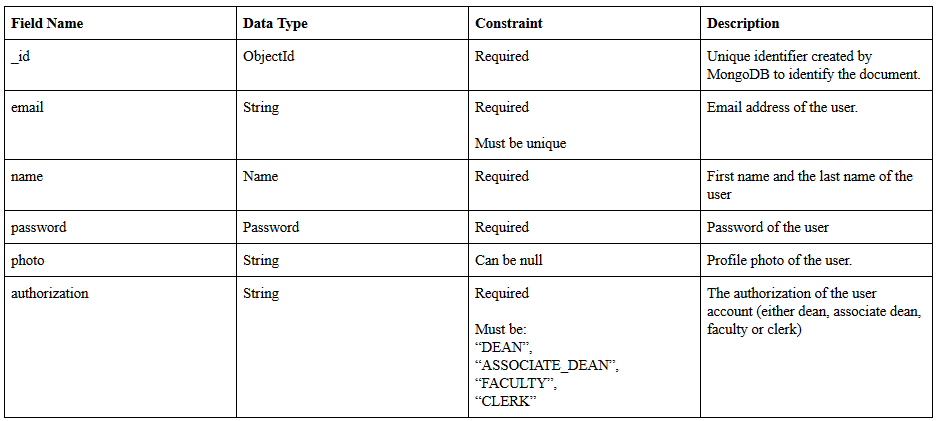
\includegraphics[width=\linewidth]{figures/tables/user_table.png}
}

Name Table
\makefigure{!ht}{
   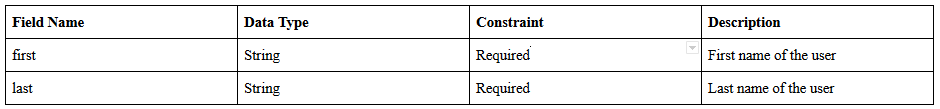
\includegraphics[width=\linewidth]{figures/tables/name_table.png}
}

Password Table
\makefigure{!ht}{
   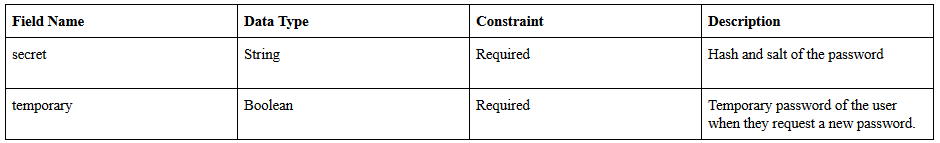
\includegraphics[width=\linewidth]{figures/tables/password_table.png}
}

\pagebreak

\subsubsection{Faculty Collection Table}

\makefigure{!ht}{
   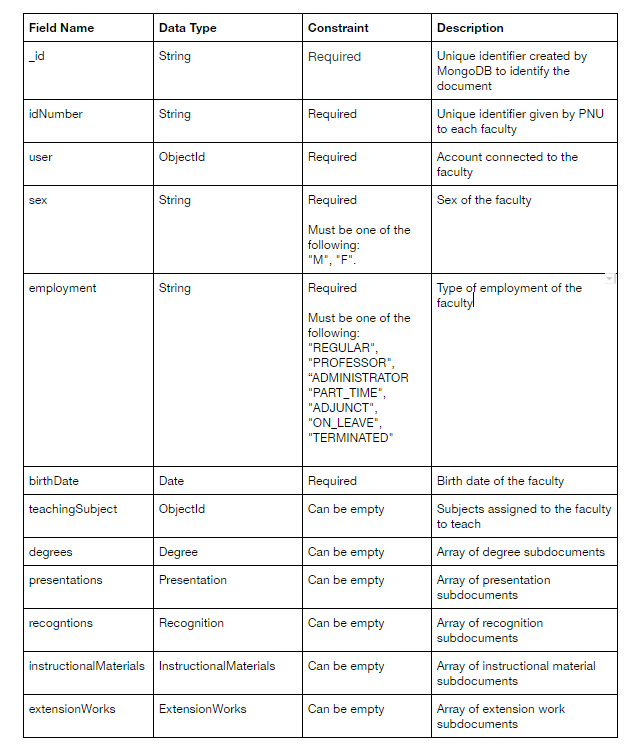
\includegraphics[scale=0.9]{figures/tables/faculty_table.png}
}

\pagebreak

\subsubsection{Faculty Subdocuments Tables}

Degree Table
\makefigure{!ht}{
   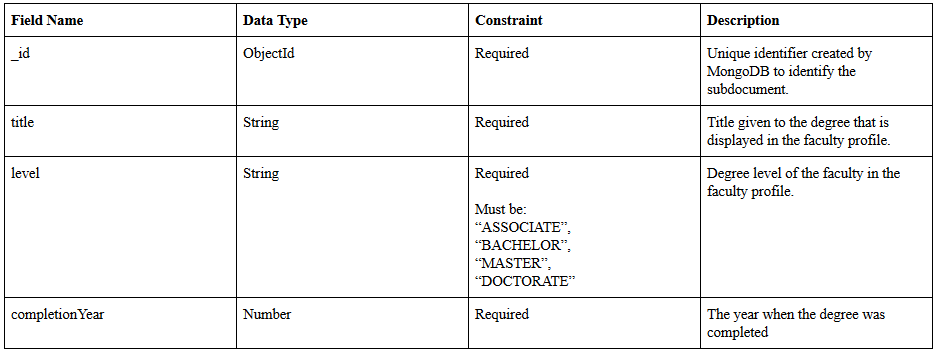
\includegraphics[width=\linewidth]{figures/tables/degree_table.png}
}

\pagebreak


Presentation Table
\makefigure{!ht}{
   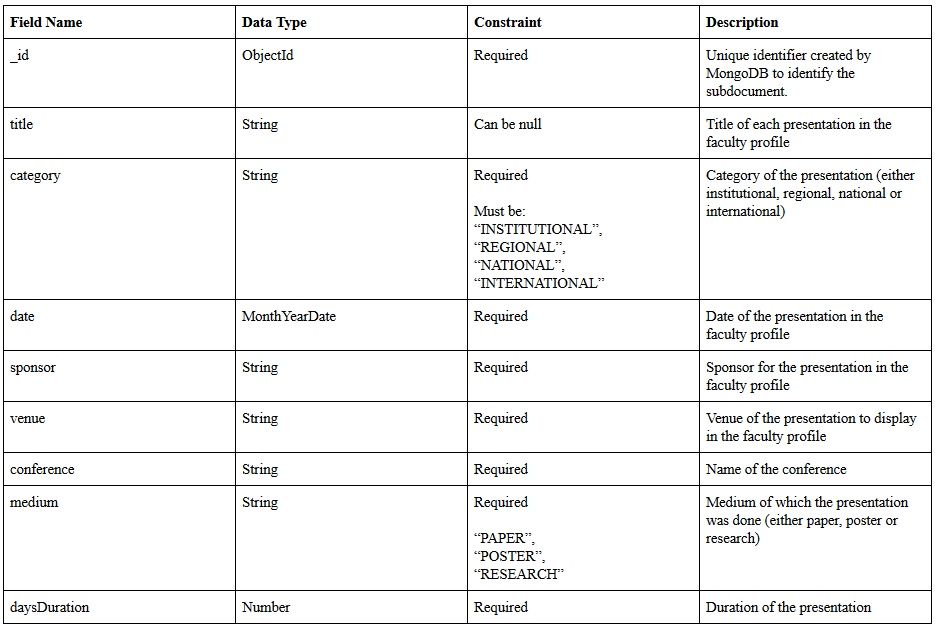
\includegraphics[width=\linewidth]{figures/tables/presentation_table.png}
}

\pagebreak


Recognition Table
\makefigure{!ht}{
   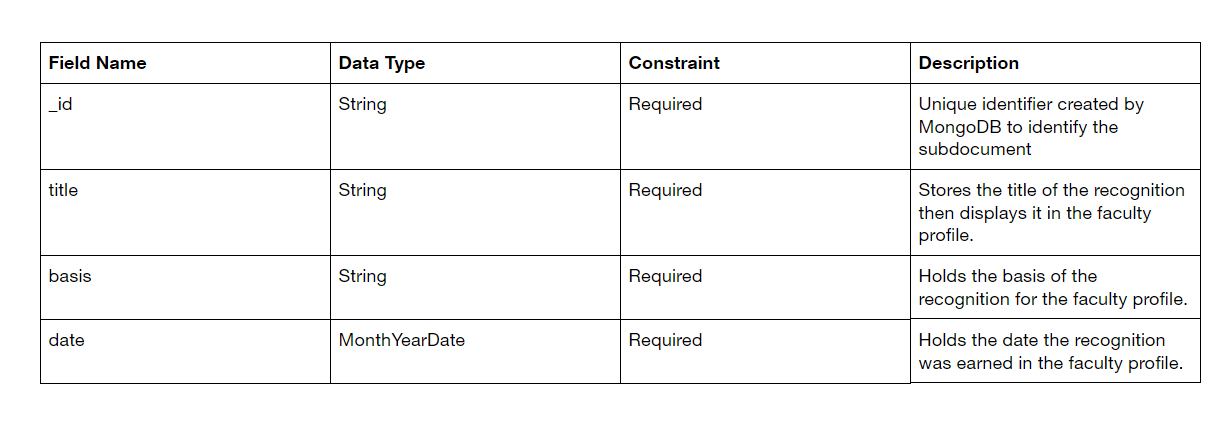
\includegraphics[width=\linewidth]{figures/tables/recognition_table.png}
}

MonthYearDate Table
\makefigure{!ht}{
   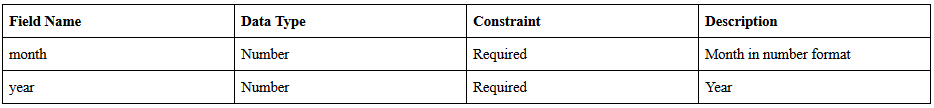
\includegraphics[width=\linewidth]{figures/tables/monthyeardate_table.png}
}

\pagebreak

InstructionalMaterial Table
\makefigure{!ht}{
   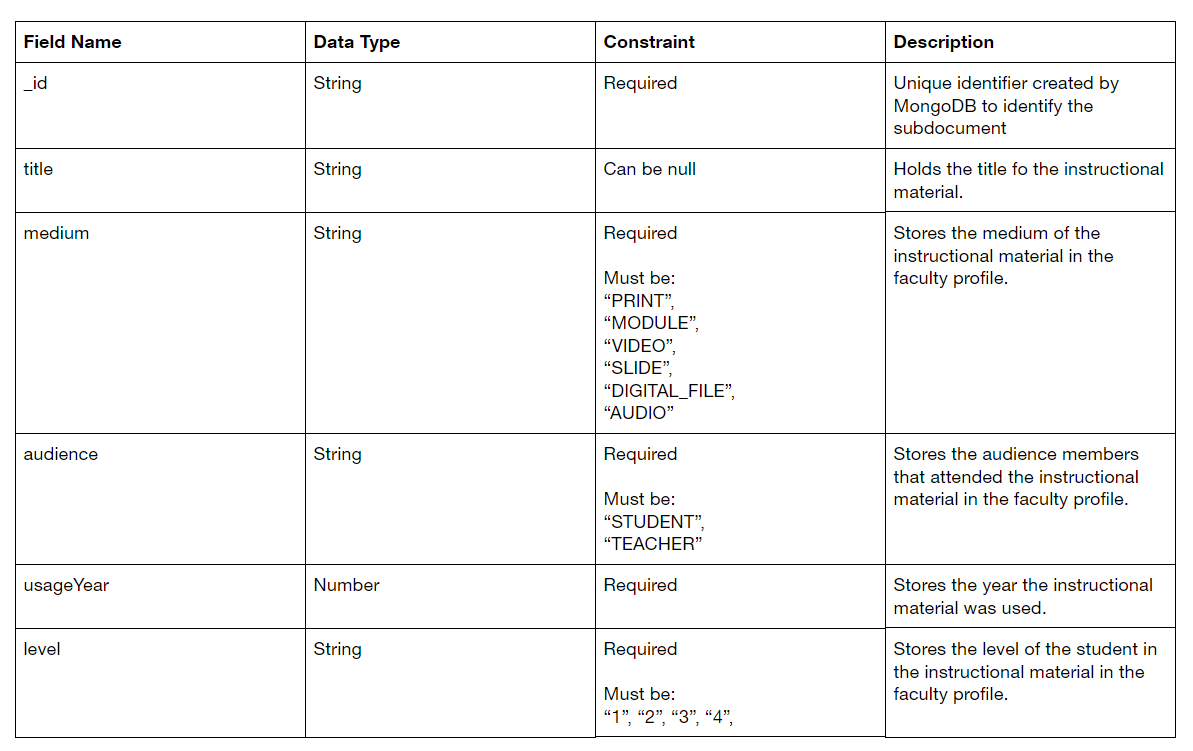
\includegraphics[width=\linewidth]{figures/tables/instructional_table.png}
}


ExtensionWork Table
\makefigure{!ht}{
   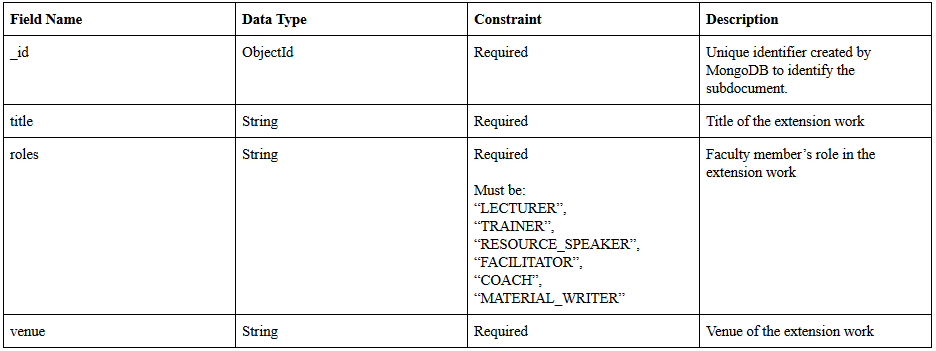
\includegraphics[width=\linewidth]{figures/tables/extension_table.png}
}

\pagebreak

\subsubsection{Subject Collection Table}
\makefigure{!ht}{
   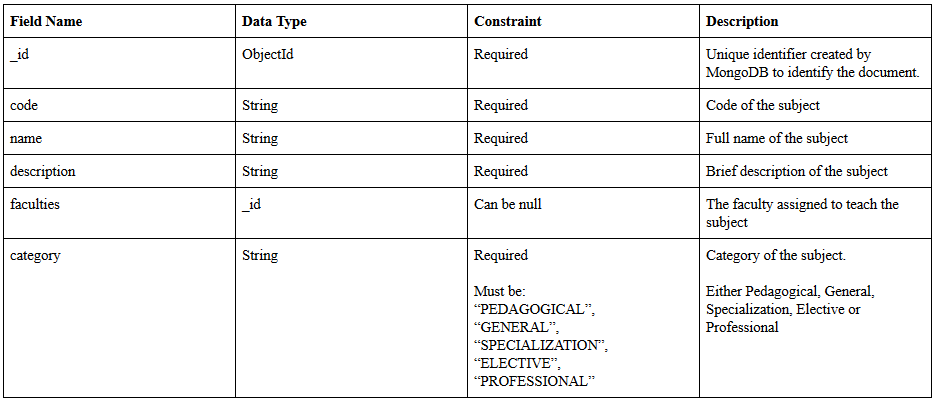
\includegraphics[width=\linewidth]{figures/tables/subject_table.png}
}


\subsubsection{TermSchedule Collection Table}
\makefigure{!ht}{
   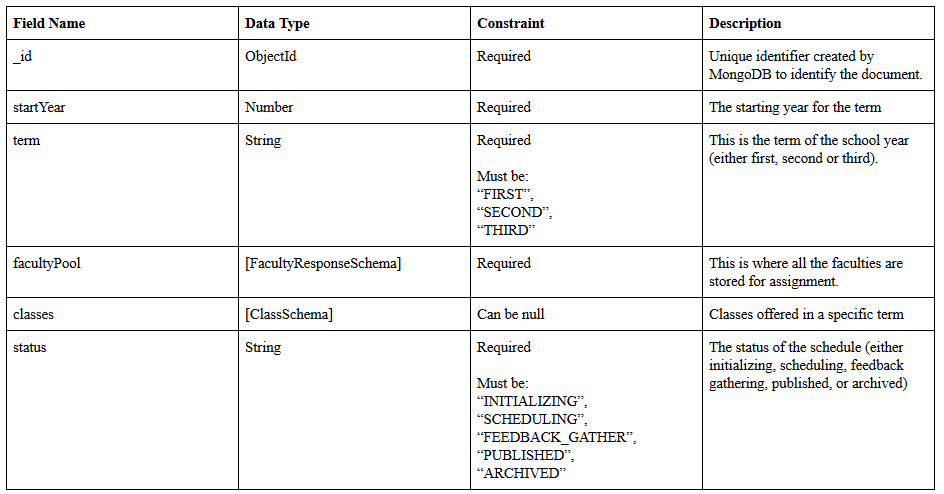
\includegraphics[width=\linewidth]{figures/tables/termschedule_table.png}
}

\pagebreak

\subsubsection{TermSchedule Subdocument Tables}

Class Table
\makefigure{!ht}{
   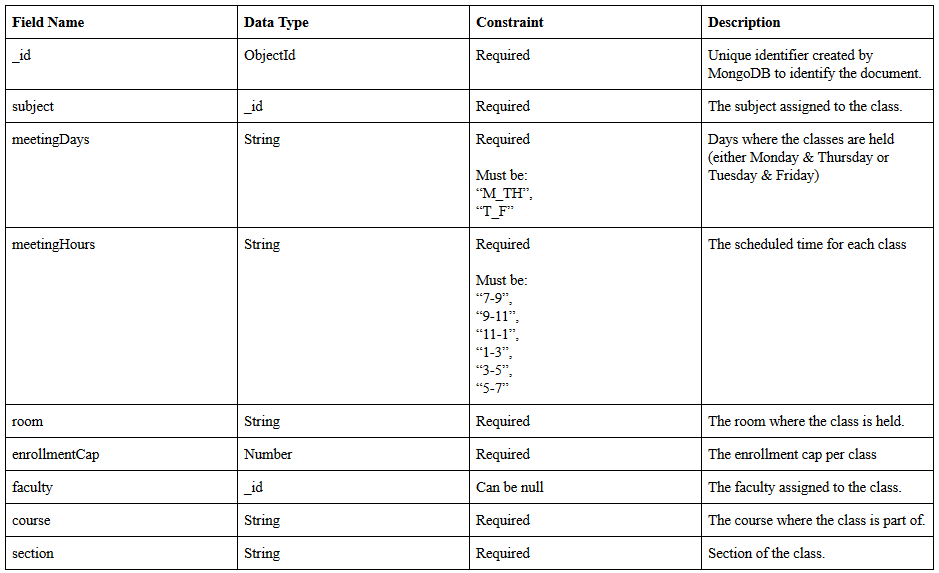
\includegraphics[width=\linewidth]{figures/tables/class_table.png}
}


FacultyResponse Table
\makefigure{!ht}{
   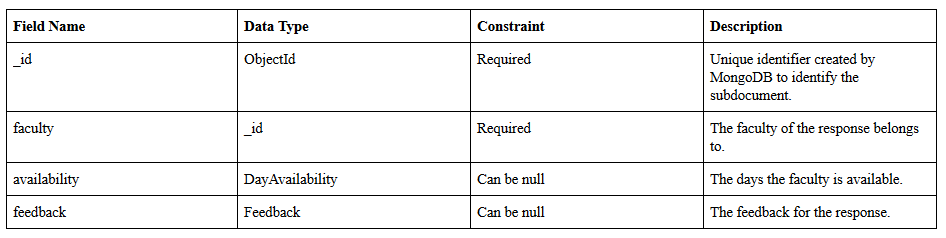
\includegraphics[width=\linewidth]{figures/tables/facultyresponse_table.png}
}

\pagebreak

DayAvailability Table
\makefigure{!ht}{
   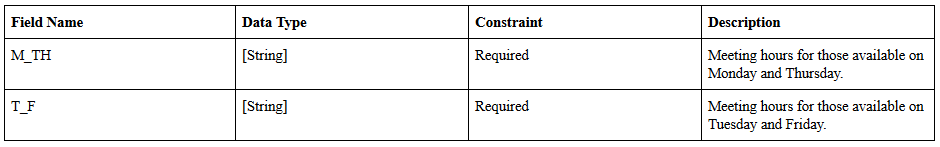
\includegraphics[width=\linewidth]{figures/tables/dayavailability_table.png}
}


Feedback Table
\makefigure{!ht}{
   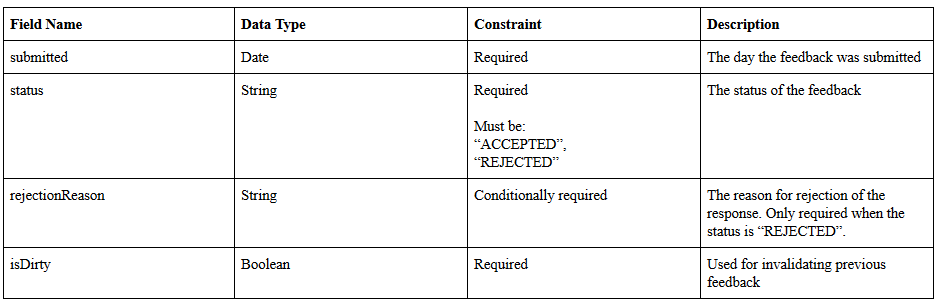
\includegraphics[width=\linewidth]{figures/tables/feedback_table.png}
}

\pagebreak

\subsection{Data Coding Standards}

\subsubsection{JavaScript}
\paragraph{Terminating statements}
Semicolons are mandatory whenever terminating a statement in JavaScript. 

\paragraph{Trailing Commas}
In object literals, array literals, function parameters, function call arguments, class extensions, module imports, and the like, trailing commas are mandatory, but only when the literal is written in multiple lines. Single line literals must not have trailing commas.

\paragraph{Module Exports}
Modules must never be exported as default. Even if a file contains only one import, it must still be exported without the default modifier. This ensures name consistency across imports, and allows IDEs to assist in module imports.

\paragraph{Variable Declarations}
Variable declarations must never be declared using the JavaScript keyword \texttt{var}. The default variable declaration should use \texttt{const}, and only changed to \texttt{let} when the variable is expected to change.

\paragraph{Utilities}
Functions and reusable code that do not belong in a particular module, but should be abstracted are classified as a utility. These utilities are given their own folder in both the server and the client and must be stored in these folders.

\paragraph{File and Folder Naming}
Files and Folders must be in snake case. 

\paragraph{Classes Naming}
Classes must be in pascal case.

\paragraph{Functions and Variable Naming}
Functions and variables must be in camel case.

\paragraph{Spaces}
Indentations must be done with 4 spaces and not tabs.

\paragraph{Arrow Functions}
Arrow functions are used to make the code shorter and more readable.

\subsubsection{Client}

\paragraph{Exporting React Components}
React components must be enclosed in their own folder. The snake case convention is overridden in this scenario; the folder and the file that contain the React component must use the same name as the React component itself. The folder must include an \texttt{index.js} file which exposes the React Component. Any other file importing this component must import the component through the \texttt{index.js} file. This is because the \texttt{index.js} file may include styling, connection to redux, or a connection to React router.

\paragraph{React Components}
React components must be written as a pure component if possible. If the component uses lifecycle functions such as \texttt{componentWillMount()}, the component may use ES6 class syntax, inheriting from \texttt{PureComponent}. If the component is stateless and only has a render function, the component should be written in function pure component form.

\paragraph{React Component Classes Instance Functions and Properties}
Instance functions in React component classes, with the exception of lifecycle methods such as \texttt{componentWillMount()} must be written in the shorthand function syntax. Instance properties such as the default state must be written as a direct assignment.

\paragraph{URL Paths}
URL paths must be written in kebab case. 

\subsubsection{Server}
\paragraph{GraphQL Type Definitions}
GraphQL type definitions must be defined in its own separate \texttt{.graphql} files and not as JavaScript string literals. This allows text editors to perform syntax highlighting on the GraphQL code.

\pagebreak


\section{Screen Specifications}
    \subsection{Sign In}
    \field{Screen Name} {Sign In}
    
    \field{File Name}{$/pages/SignIn/index.js$}
    
    \field{Description}{Where users must enter their Email address and password to access the system.}
    
    \field{Layout}{}
    
    
\makefigure{!ht}{
   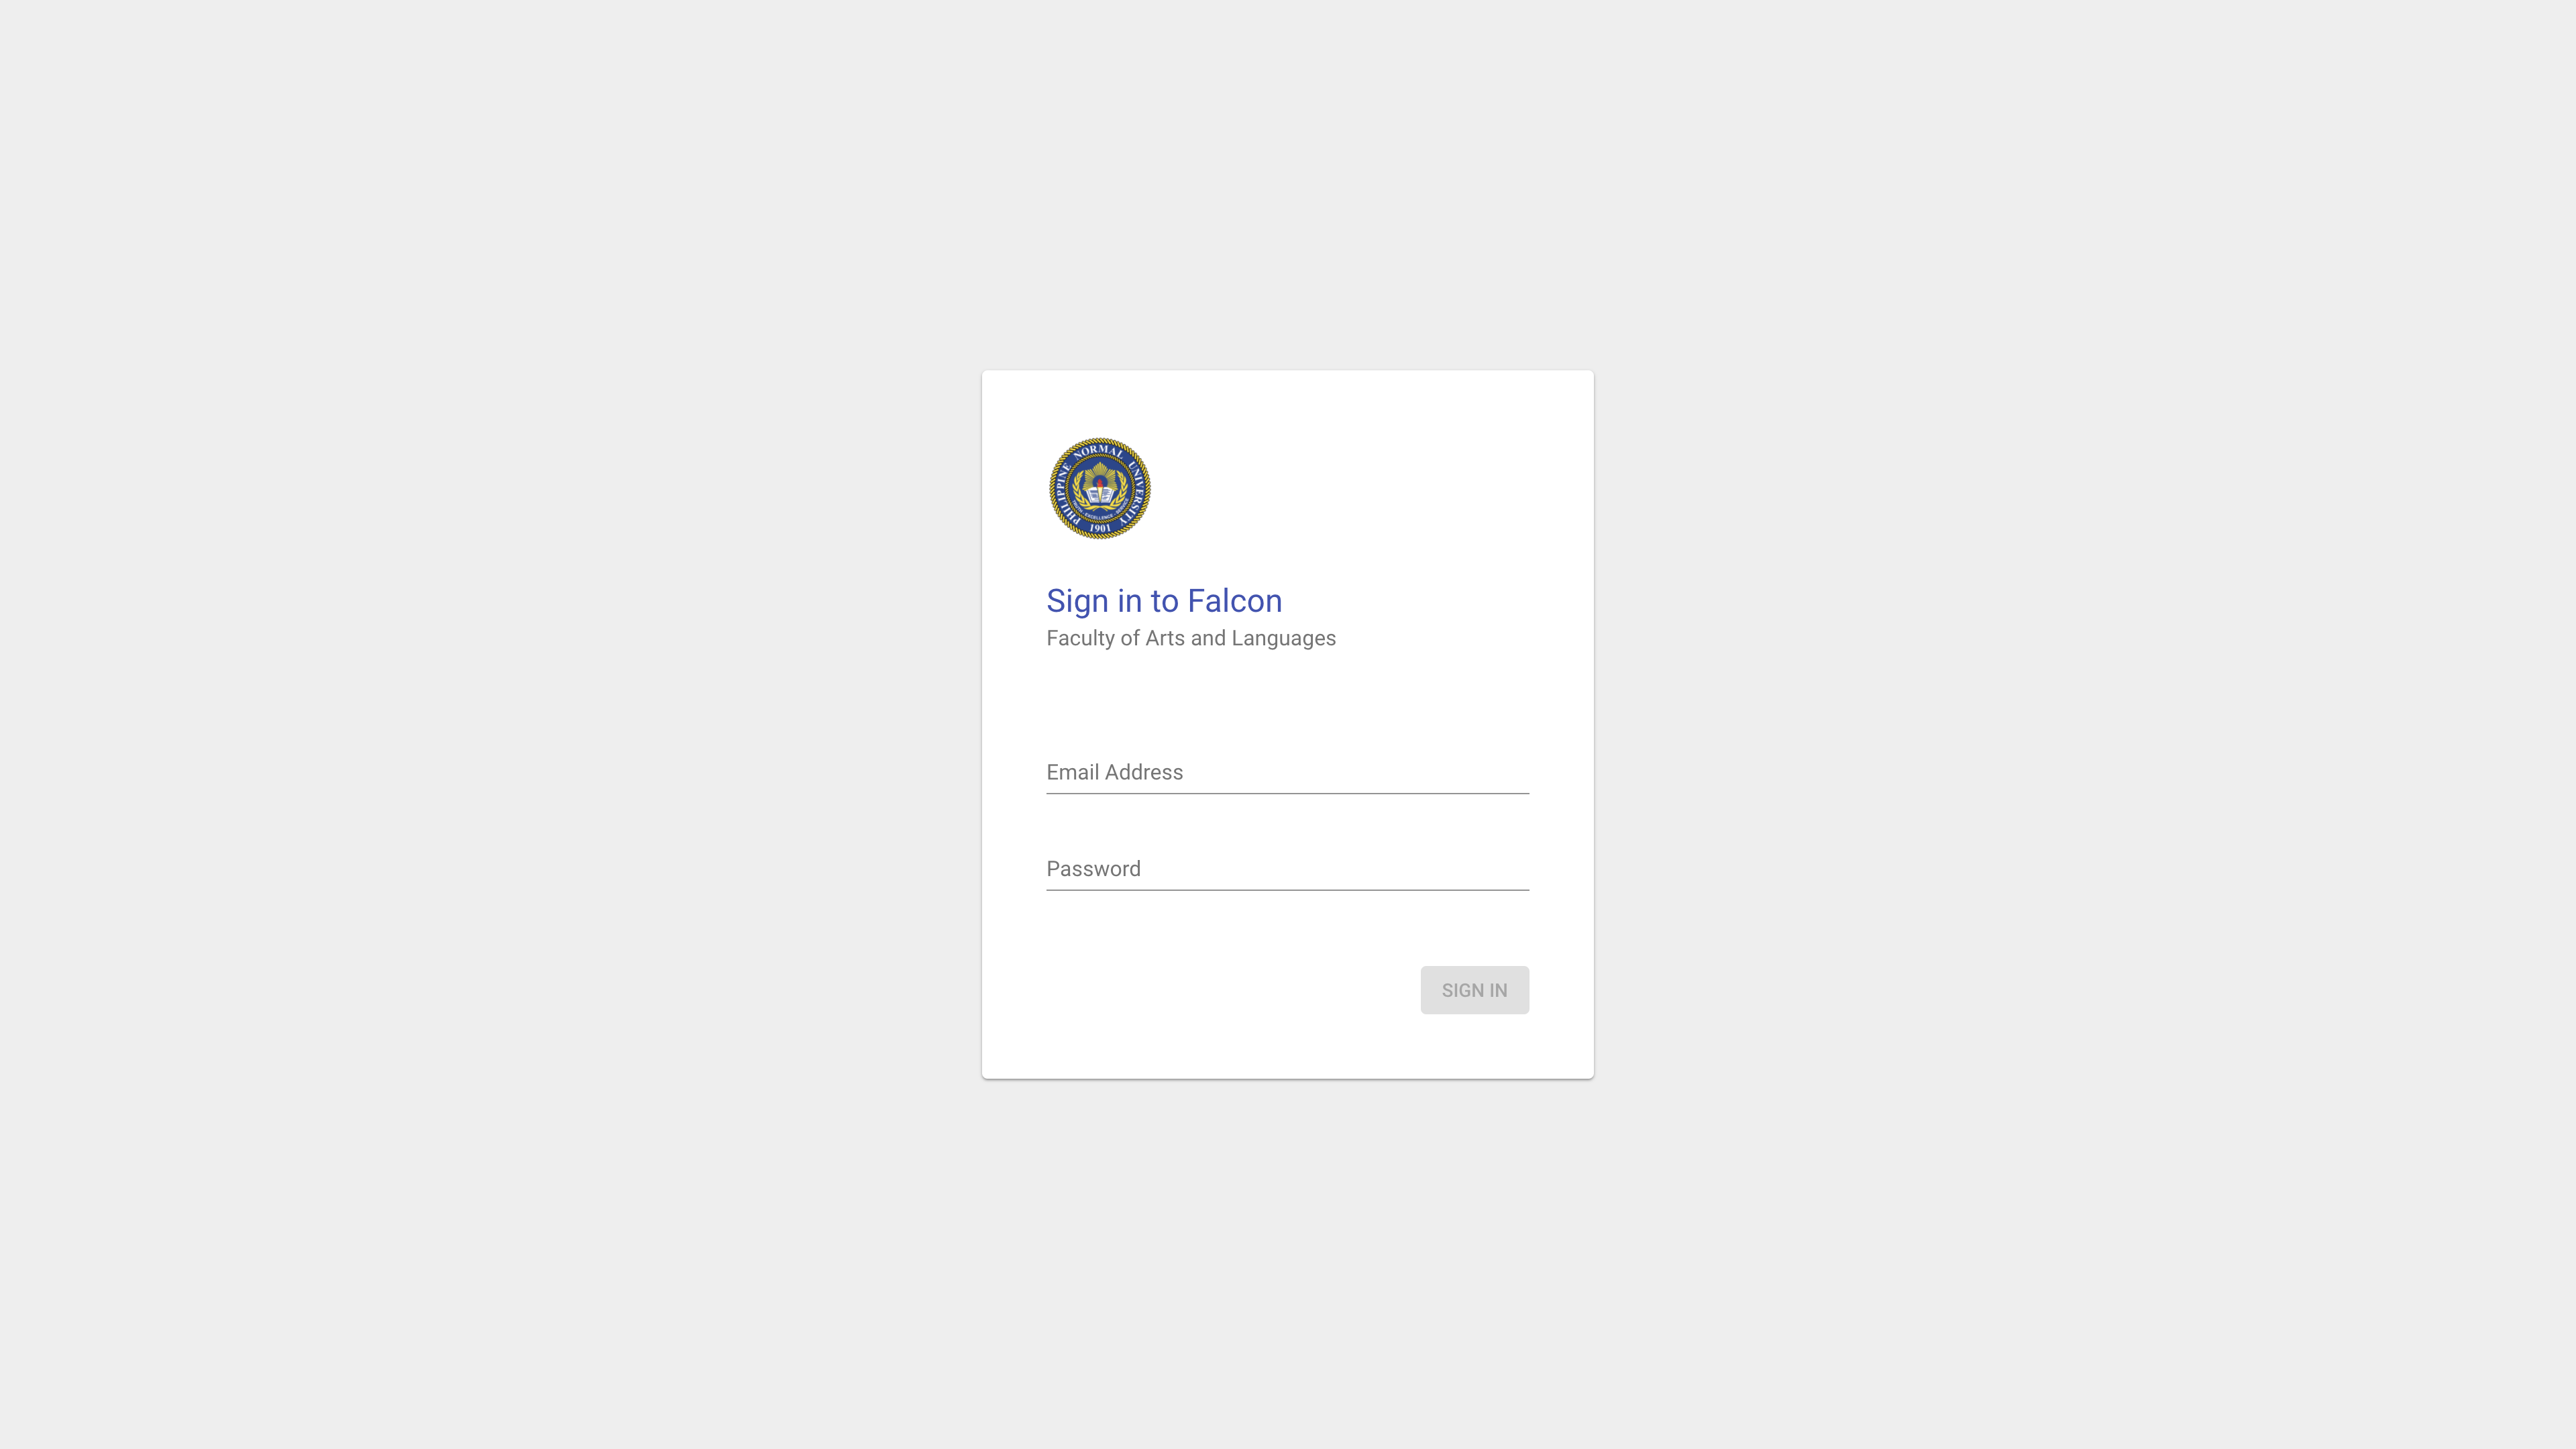
\includegraphics[width=\linewidth]{figures/screen_specifications/sign_in.png}
   \caption{Sign In Screen}
}
    \pagebreak

    \subsection{Faculty Profile}
    
    \subsubsection{Faculty Overview}
    \field{Screen Name} {Faculty Overview}
    
    \field{File Name}{$/pages/FacultyProfiles/index.js$}
    
    \field{Description}{Displays the details of the faculty member. First card contains the basic information, second card contains the subject assignments, third card contains the degrees, and fourth card contains the recognitions.}
    
    \field{Layout}{}
    
    
\makefigure{!ht}{
   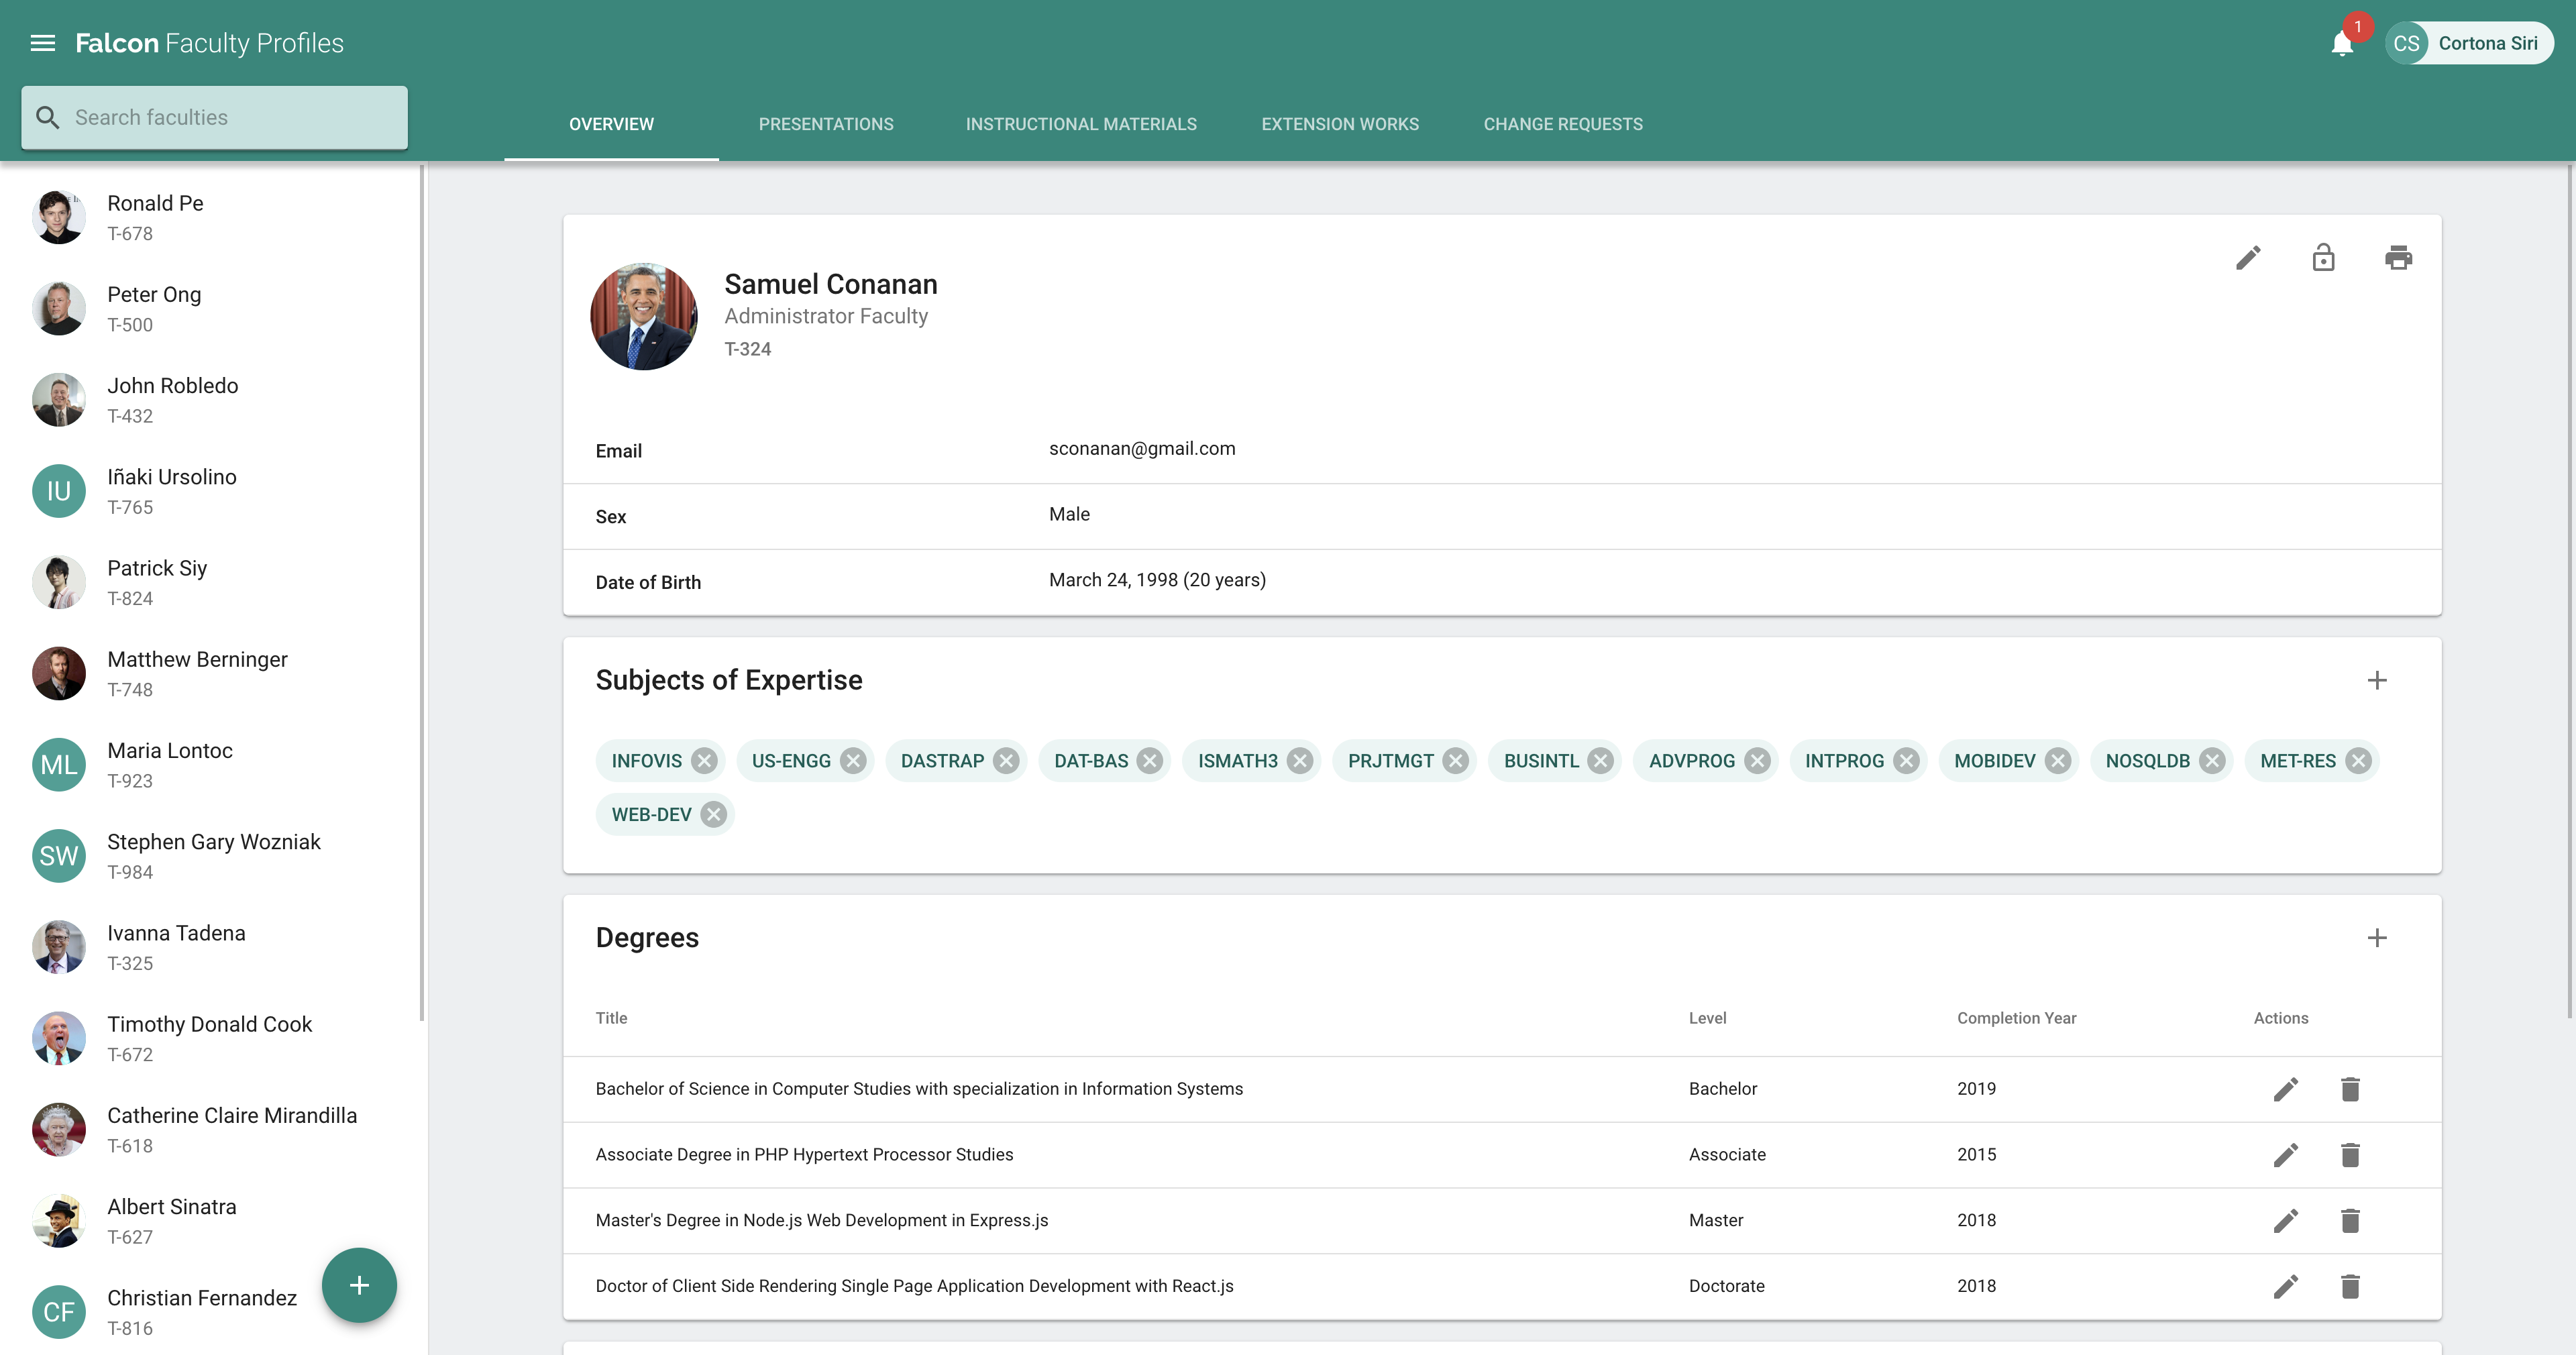
\includegraphics[width=\linewidth]{figures/screen_specifications/faculty_profile1.png}
   \caption{Faculty Profile Screen A}
}

\pagebreak

\makefigure{!ht}{
   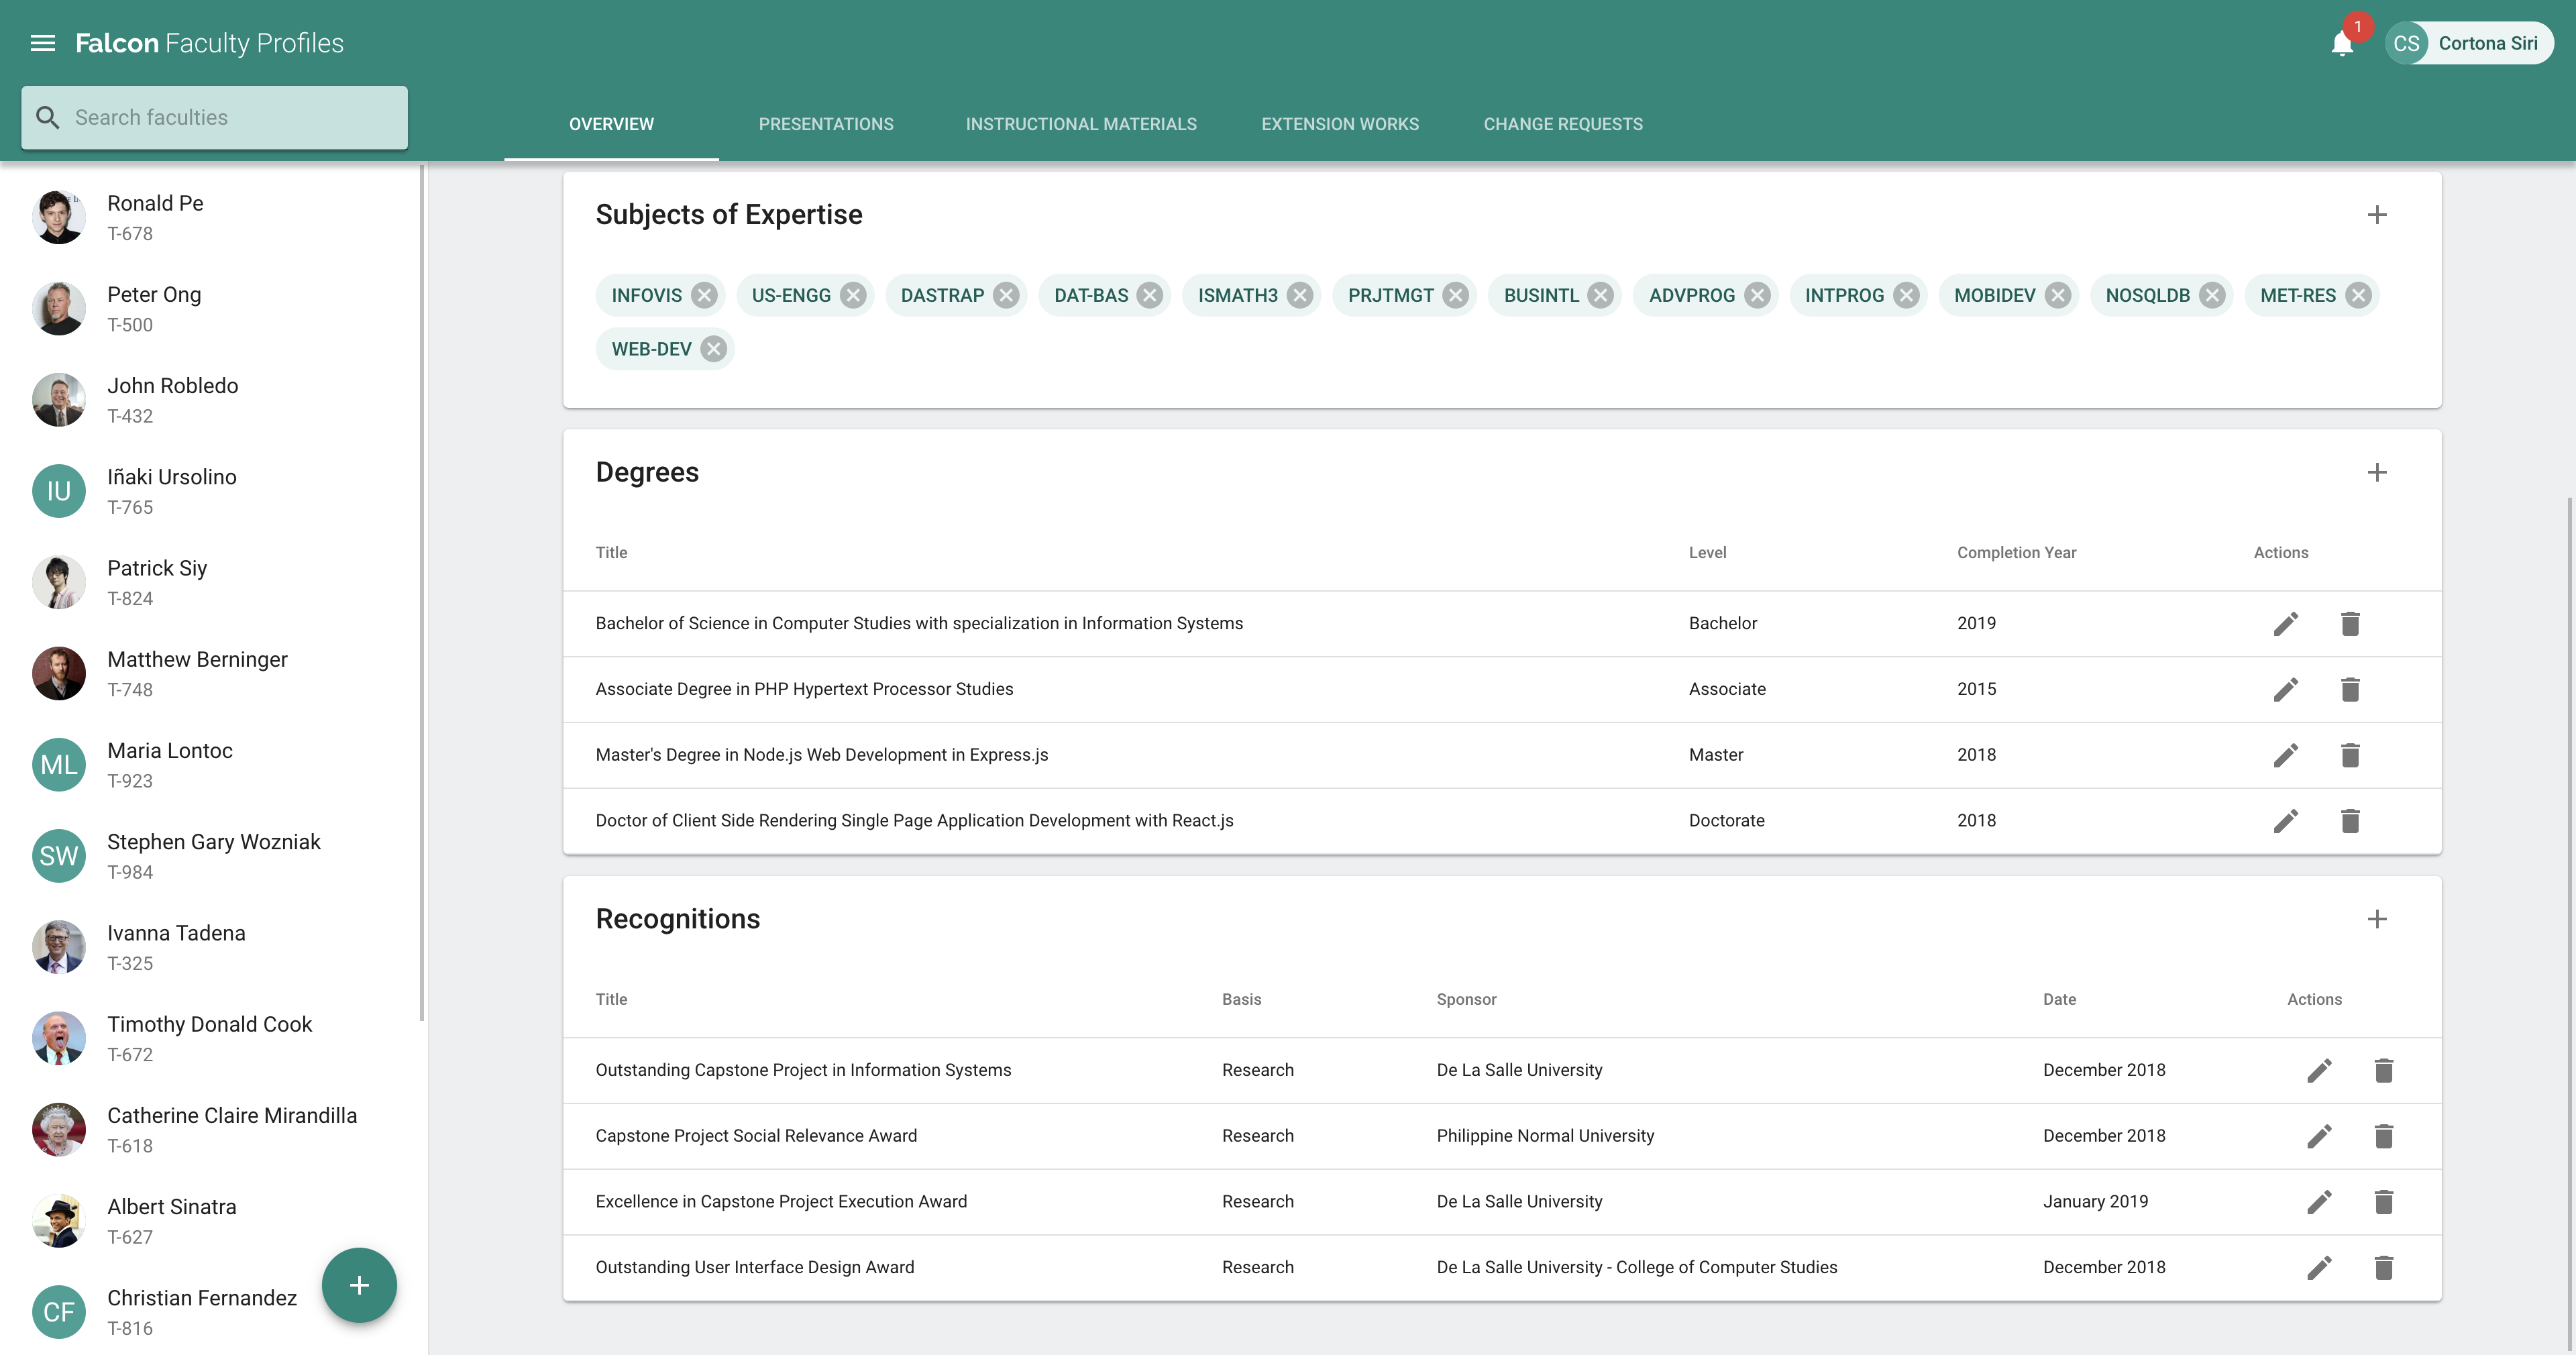
\includegraphics[width=\linewidth]{figures/screen_specifications/faculty_profile2.png}
   \caption{Faculty Profile Screen B}
}

\pagebreak

\subsubsection{Remove Degree}
    
    \field{Screen Name}{Remove Degree}
    
    \field{File Name}{$/pages/FacultyProfiles/components/modals/RemoveDegreeModal/index.js$}
    
    \field{Description} {Warns the clerk or dean to confirm if they want to remove the degree from the faculty profile.}
    
    \field{Layout}{}
    
\makefigure{!ht}{
   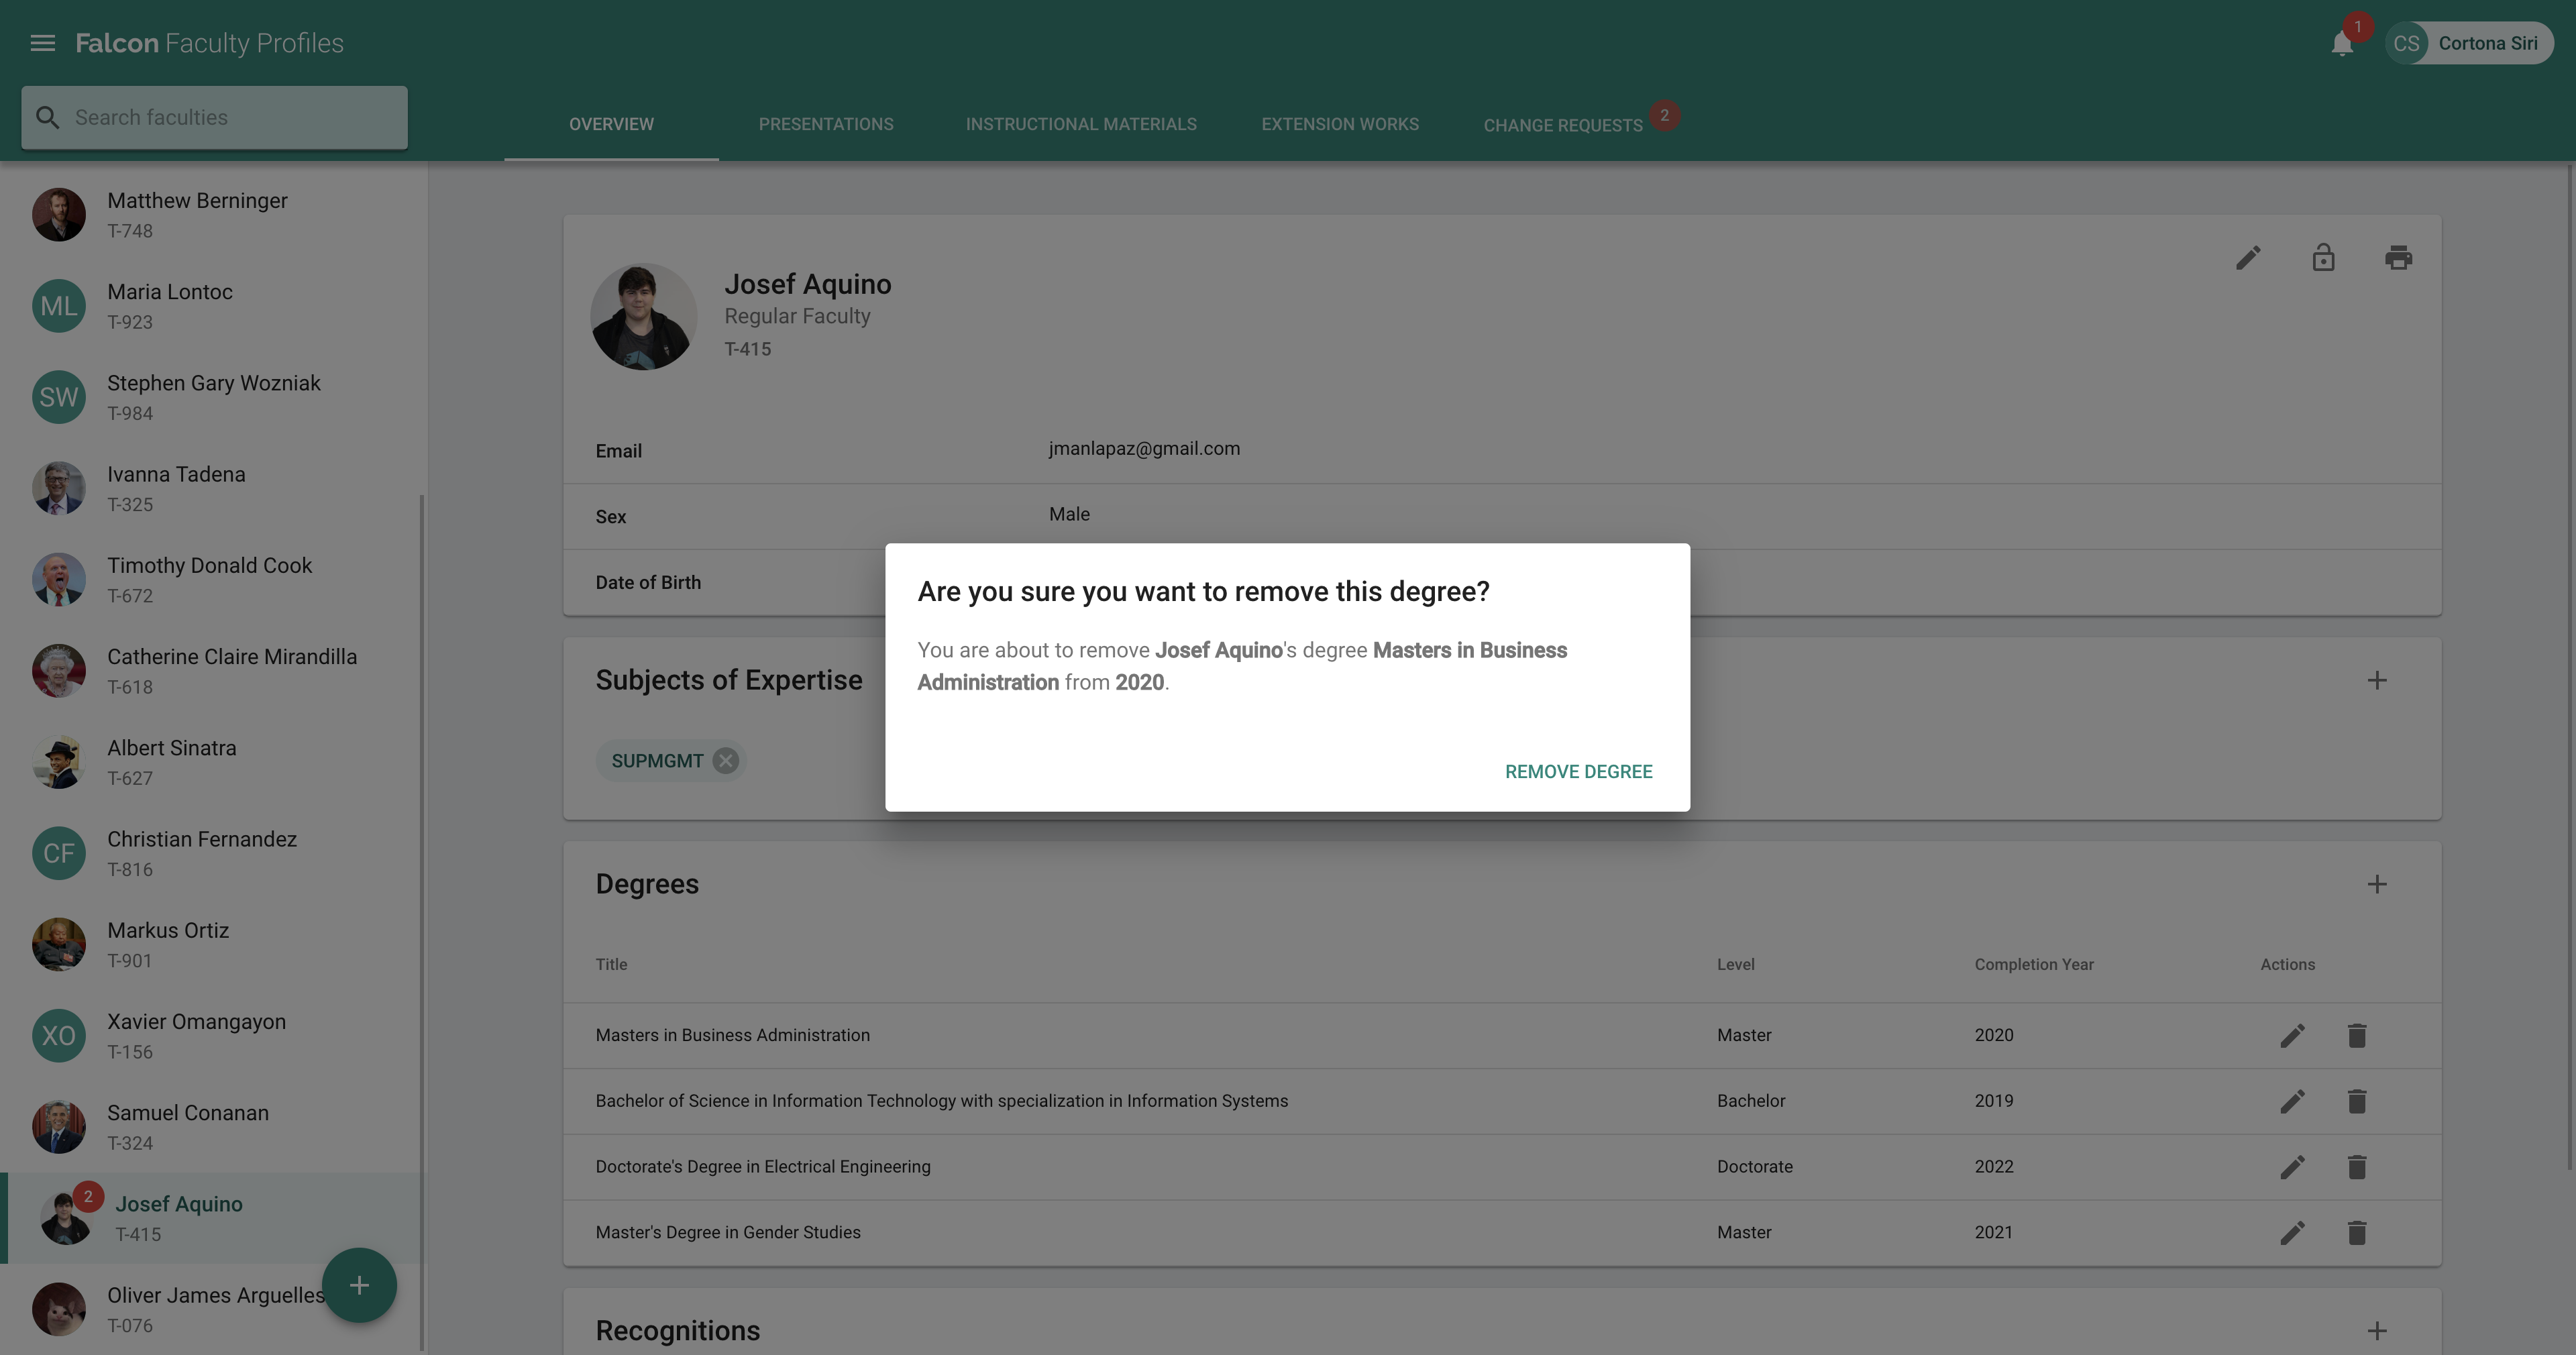
\includegraphics[width=\linewidth]{figures/screen_specifications/remove_degree.png}
   \caption{Remove Degree Screen}
   }
   
   \pagebreak
   
    \subsubsection{Remove Recognitions}
    
    \field{Screen Name}{Remove Recognitions}
    
    \field{File Name}{$/pages/FacultyProfiles/components/modals/RemoveRecognitionModal/index.js$}
    
    \field{Description} {Confirm if the clerk or dean wants to remove the recognition from the faculty profile.}
    
    \field{Layout}{}
    
\makefigure{!ht}{
   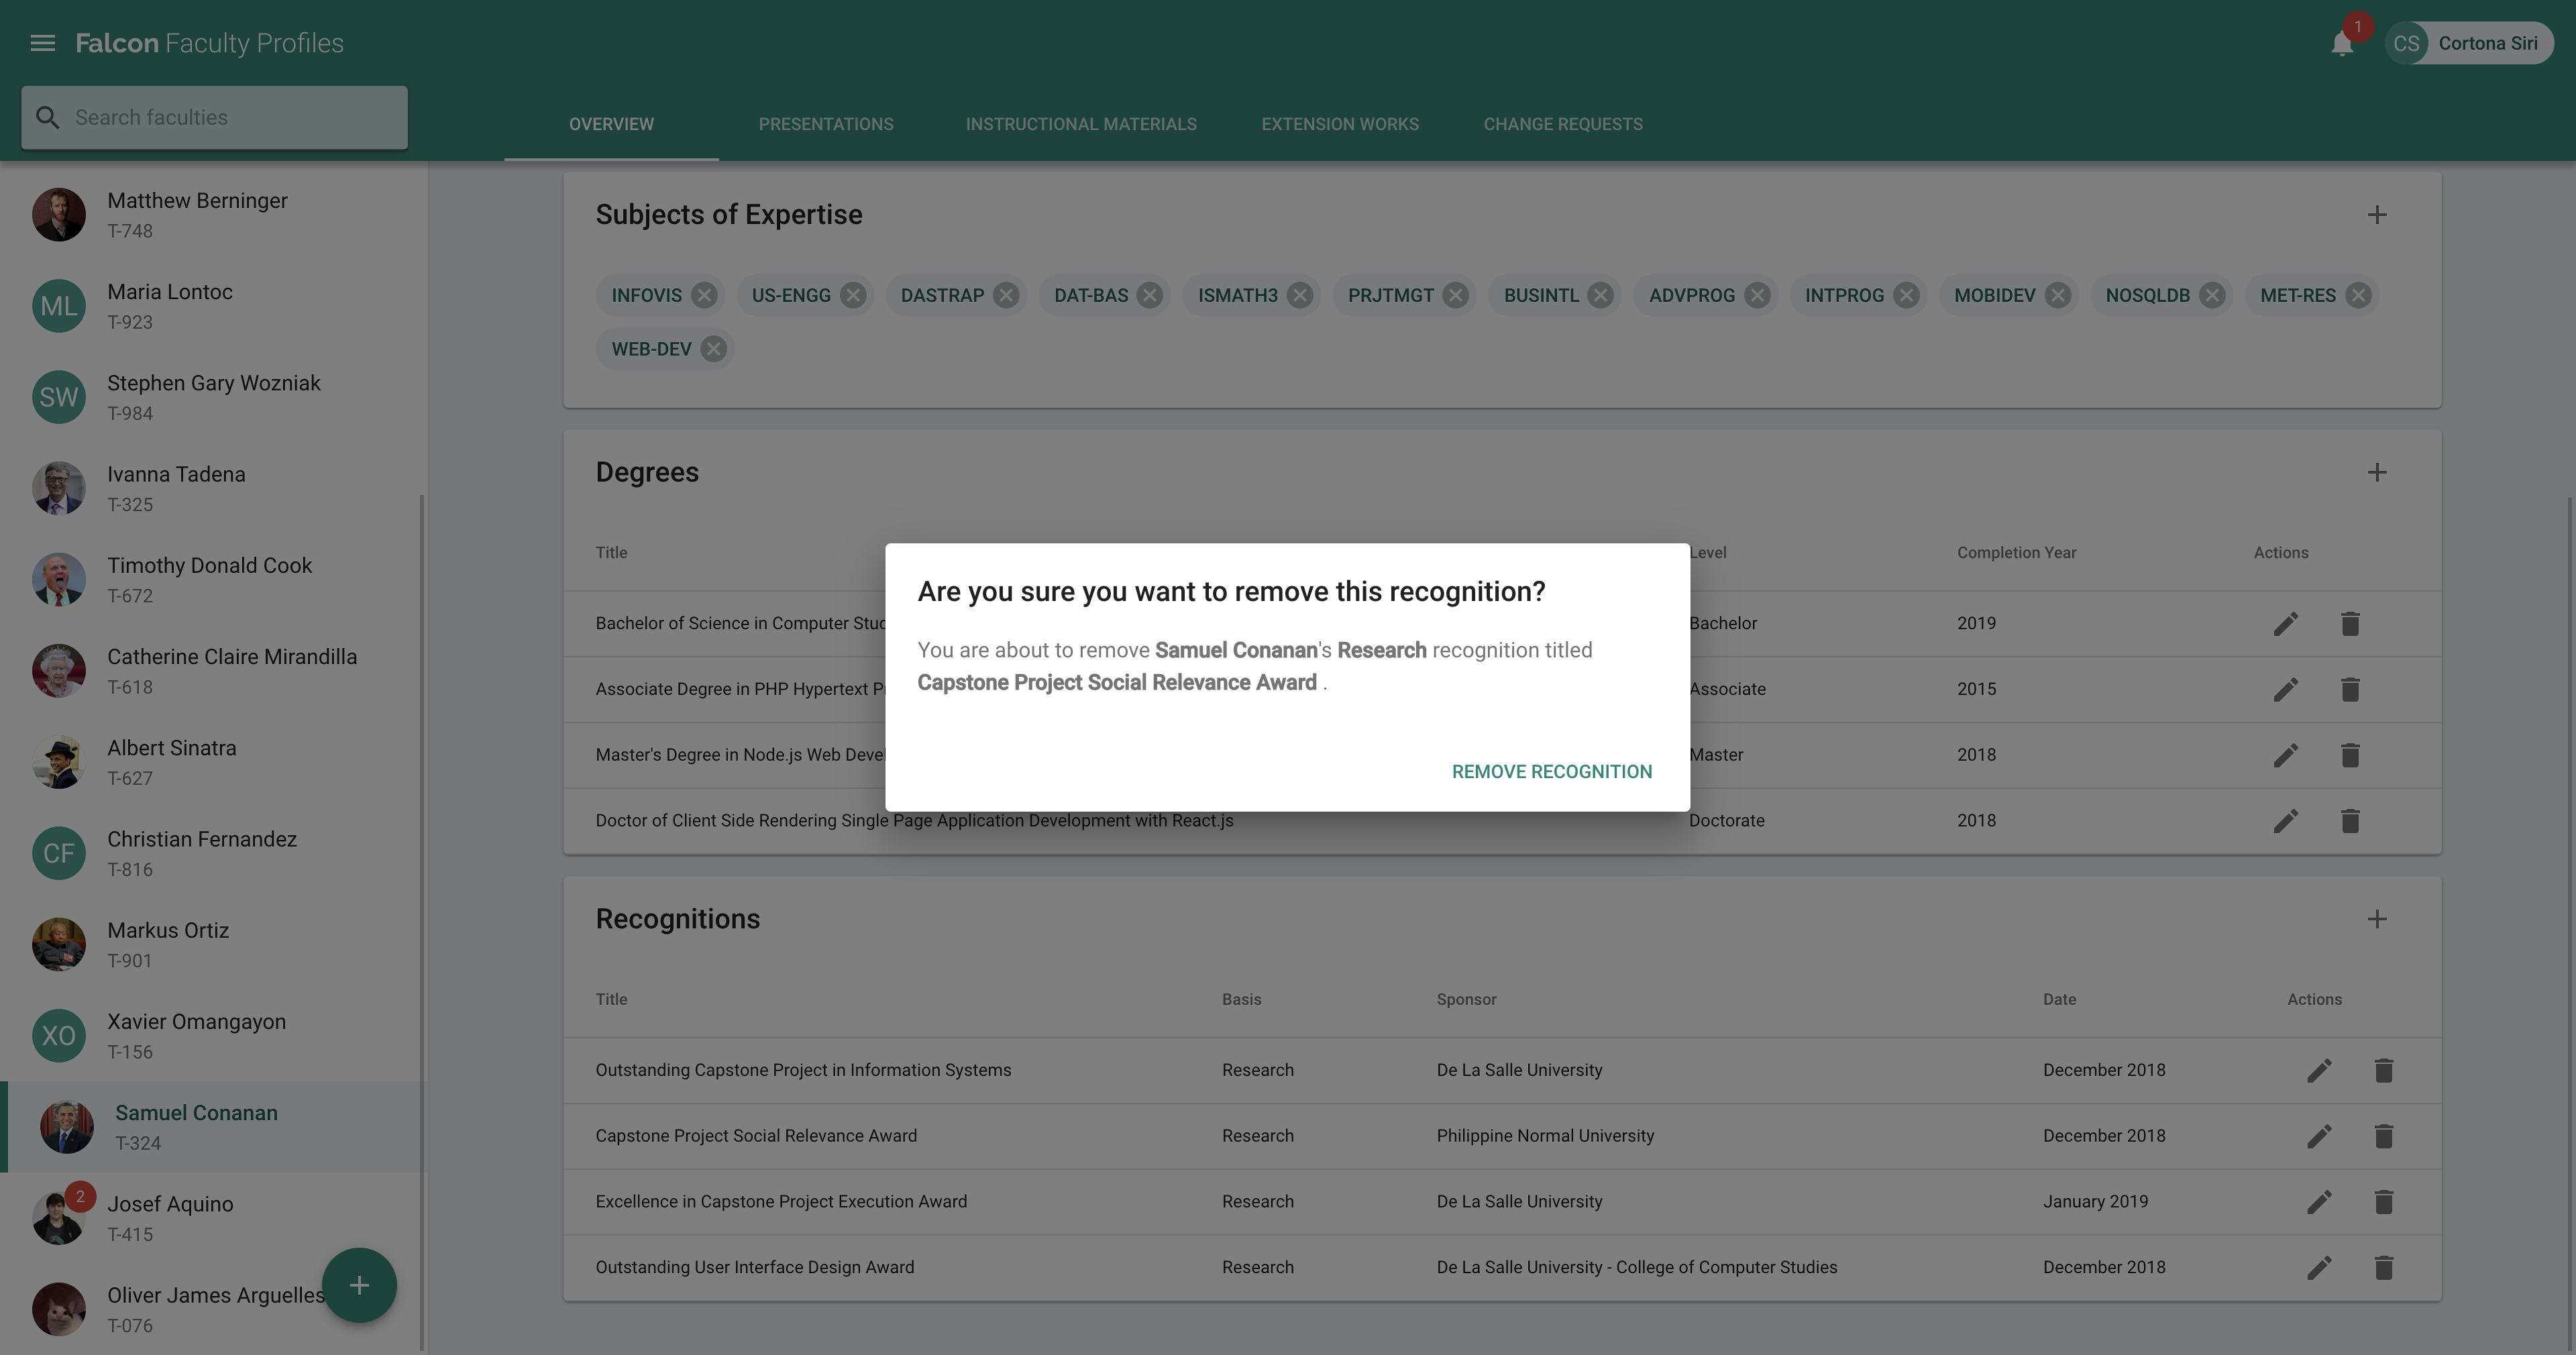
\includegraphics[width=\linewidth]{figures/screen_specifications/remove_recognition.png}
   \caption{Remove Recognition Screen}
   }
   
   \pagebreak
   
    \subsubsection{Print Preview}
    
    \field{Screen Name}{Print Preview}
    
    \field{File Name}{$/pages/FacultyProfiles/ProfilePrintPreview/index.js$}
    
    \field{Description} {Shows the clerk or dean a preview of the report. Also allows the user to select which kind of information to include in the report.}
    
    \field{Layout}{}
    
\makefigure{!ht}{
   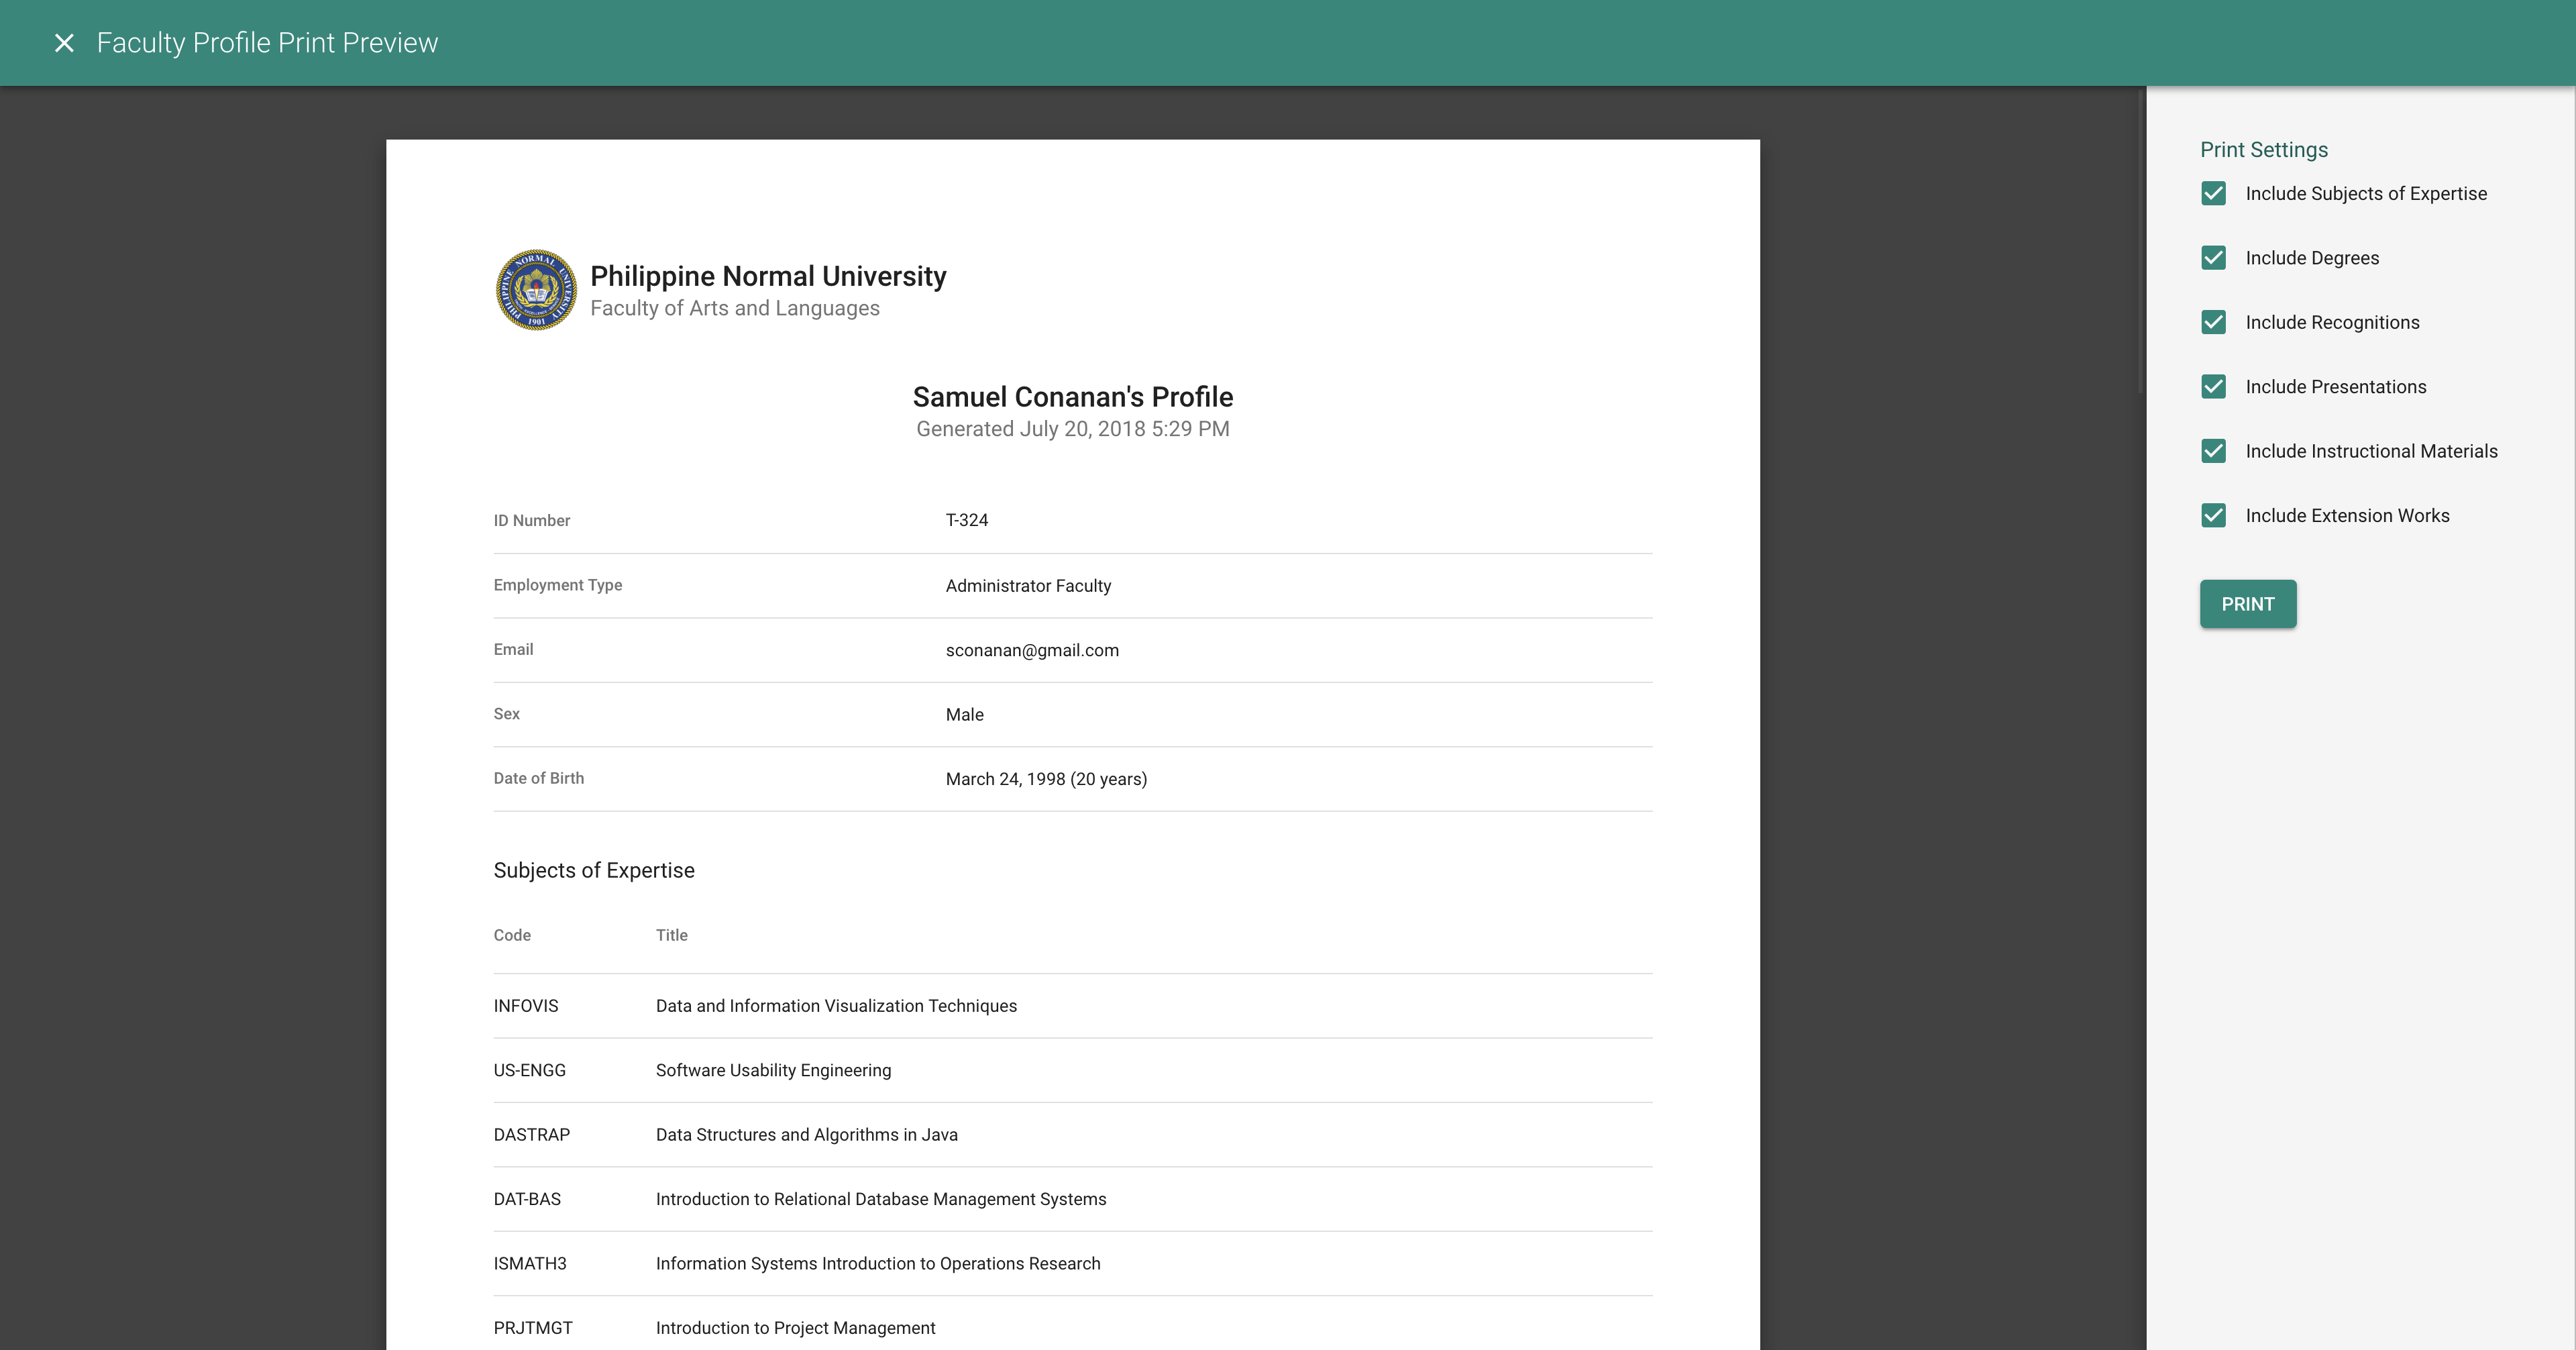
\includegraphics[width=\linewidth]{figures/screen_specifications/print_preview.png}
   \caption{Print Preview Screen}
   }
   
   \pagebreak
   
   \subsubsection{Reset Password}
    
    \field{Screen Name}{Reset Password}
    
    \field{File Name}{$/pages/FacultyProfiles/components/modals/ResetPasswordModal/index.js$}
    
    \field{Description} {Allows the clerk or dean to reset the password of a faculty member through the faculty profile.}
    
    \field{Layout}{}
    
\makefigure{!ht}{
   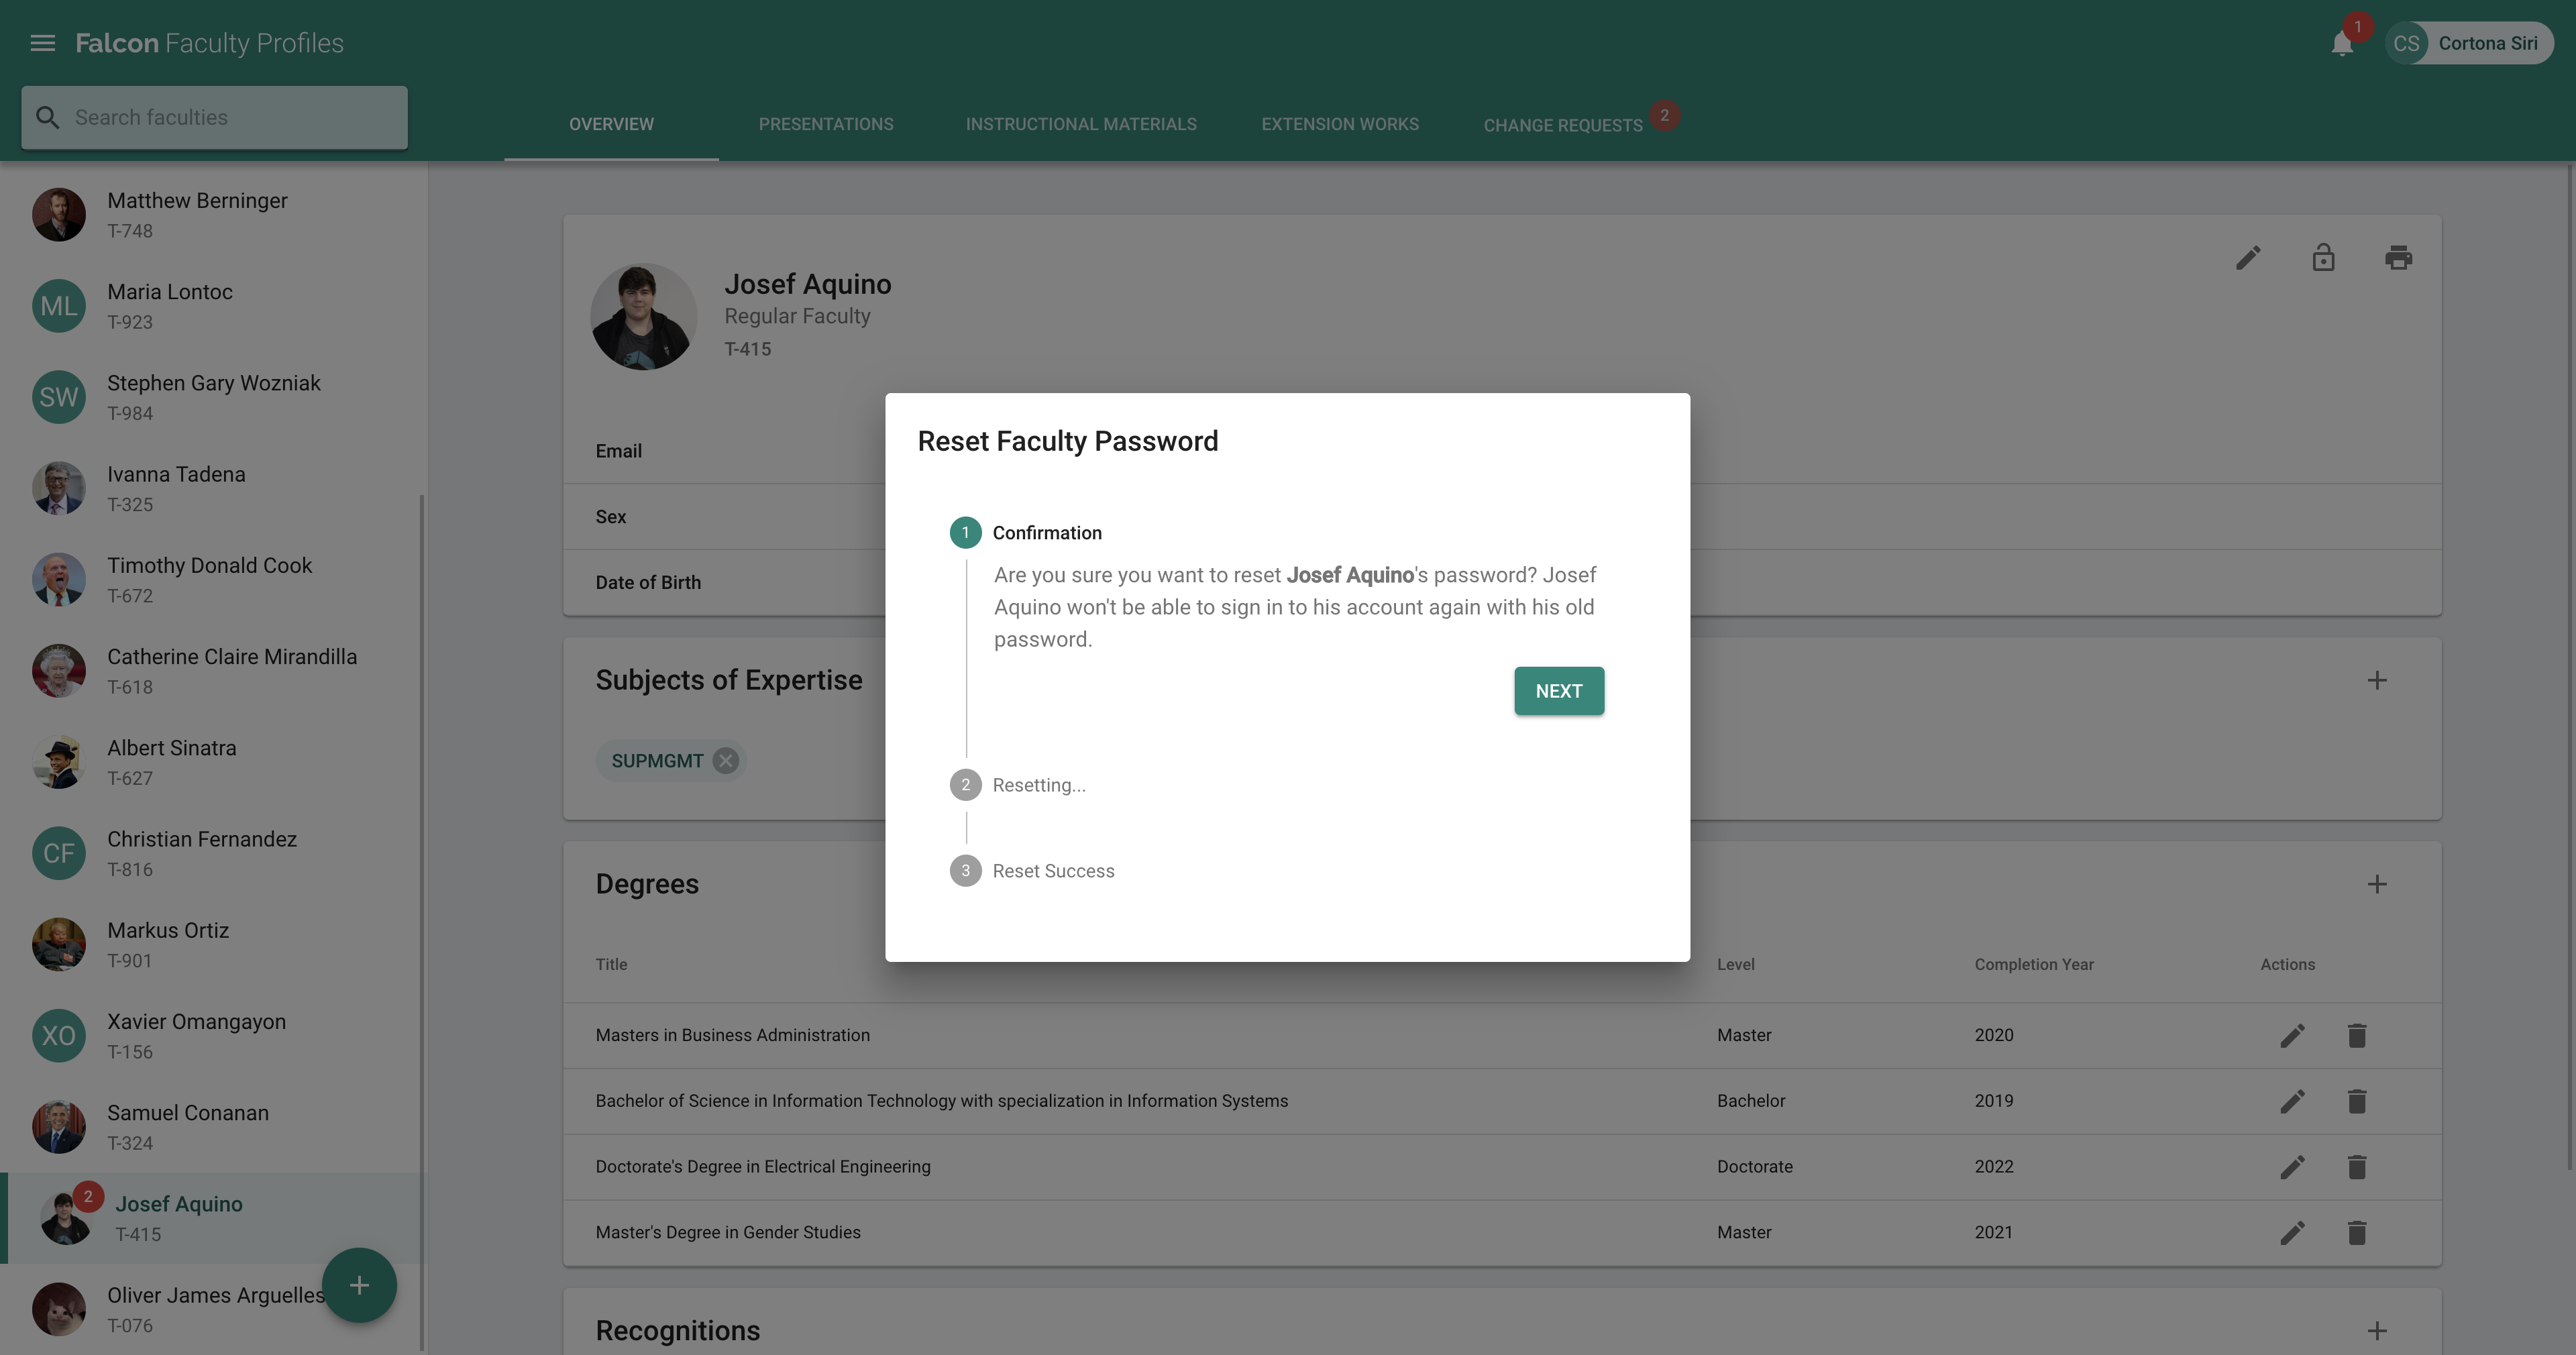
\includegraphics[width=\linewidth]{figures/screen_specifications/reset_password1.png}
   \caption{Reset Password Screen A}
   }
   \pagebreak
   
   \makefigure{!ht}{
   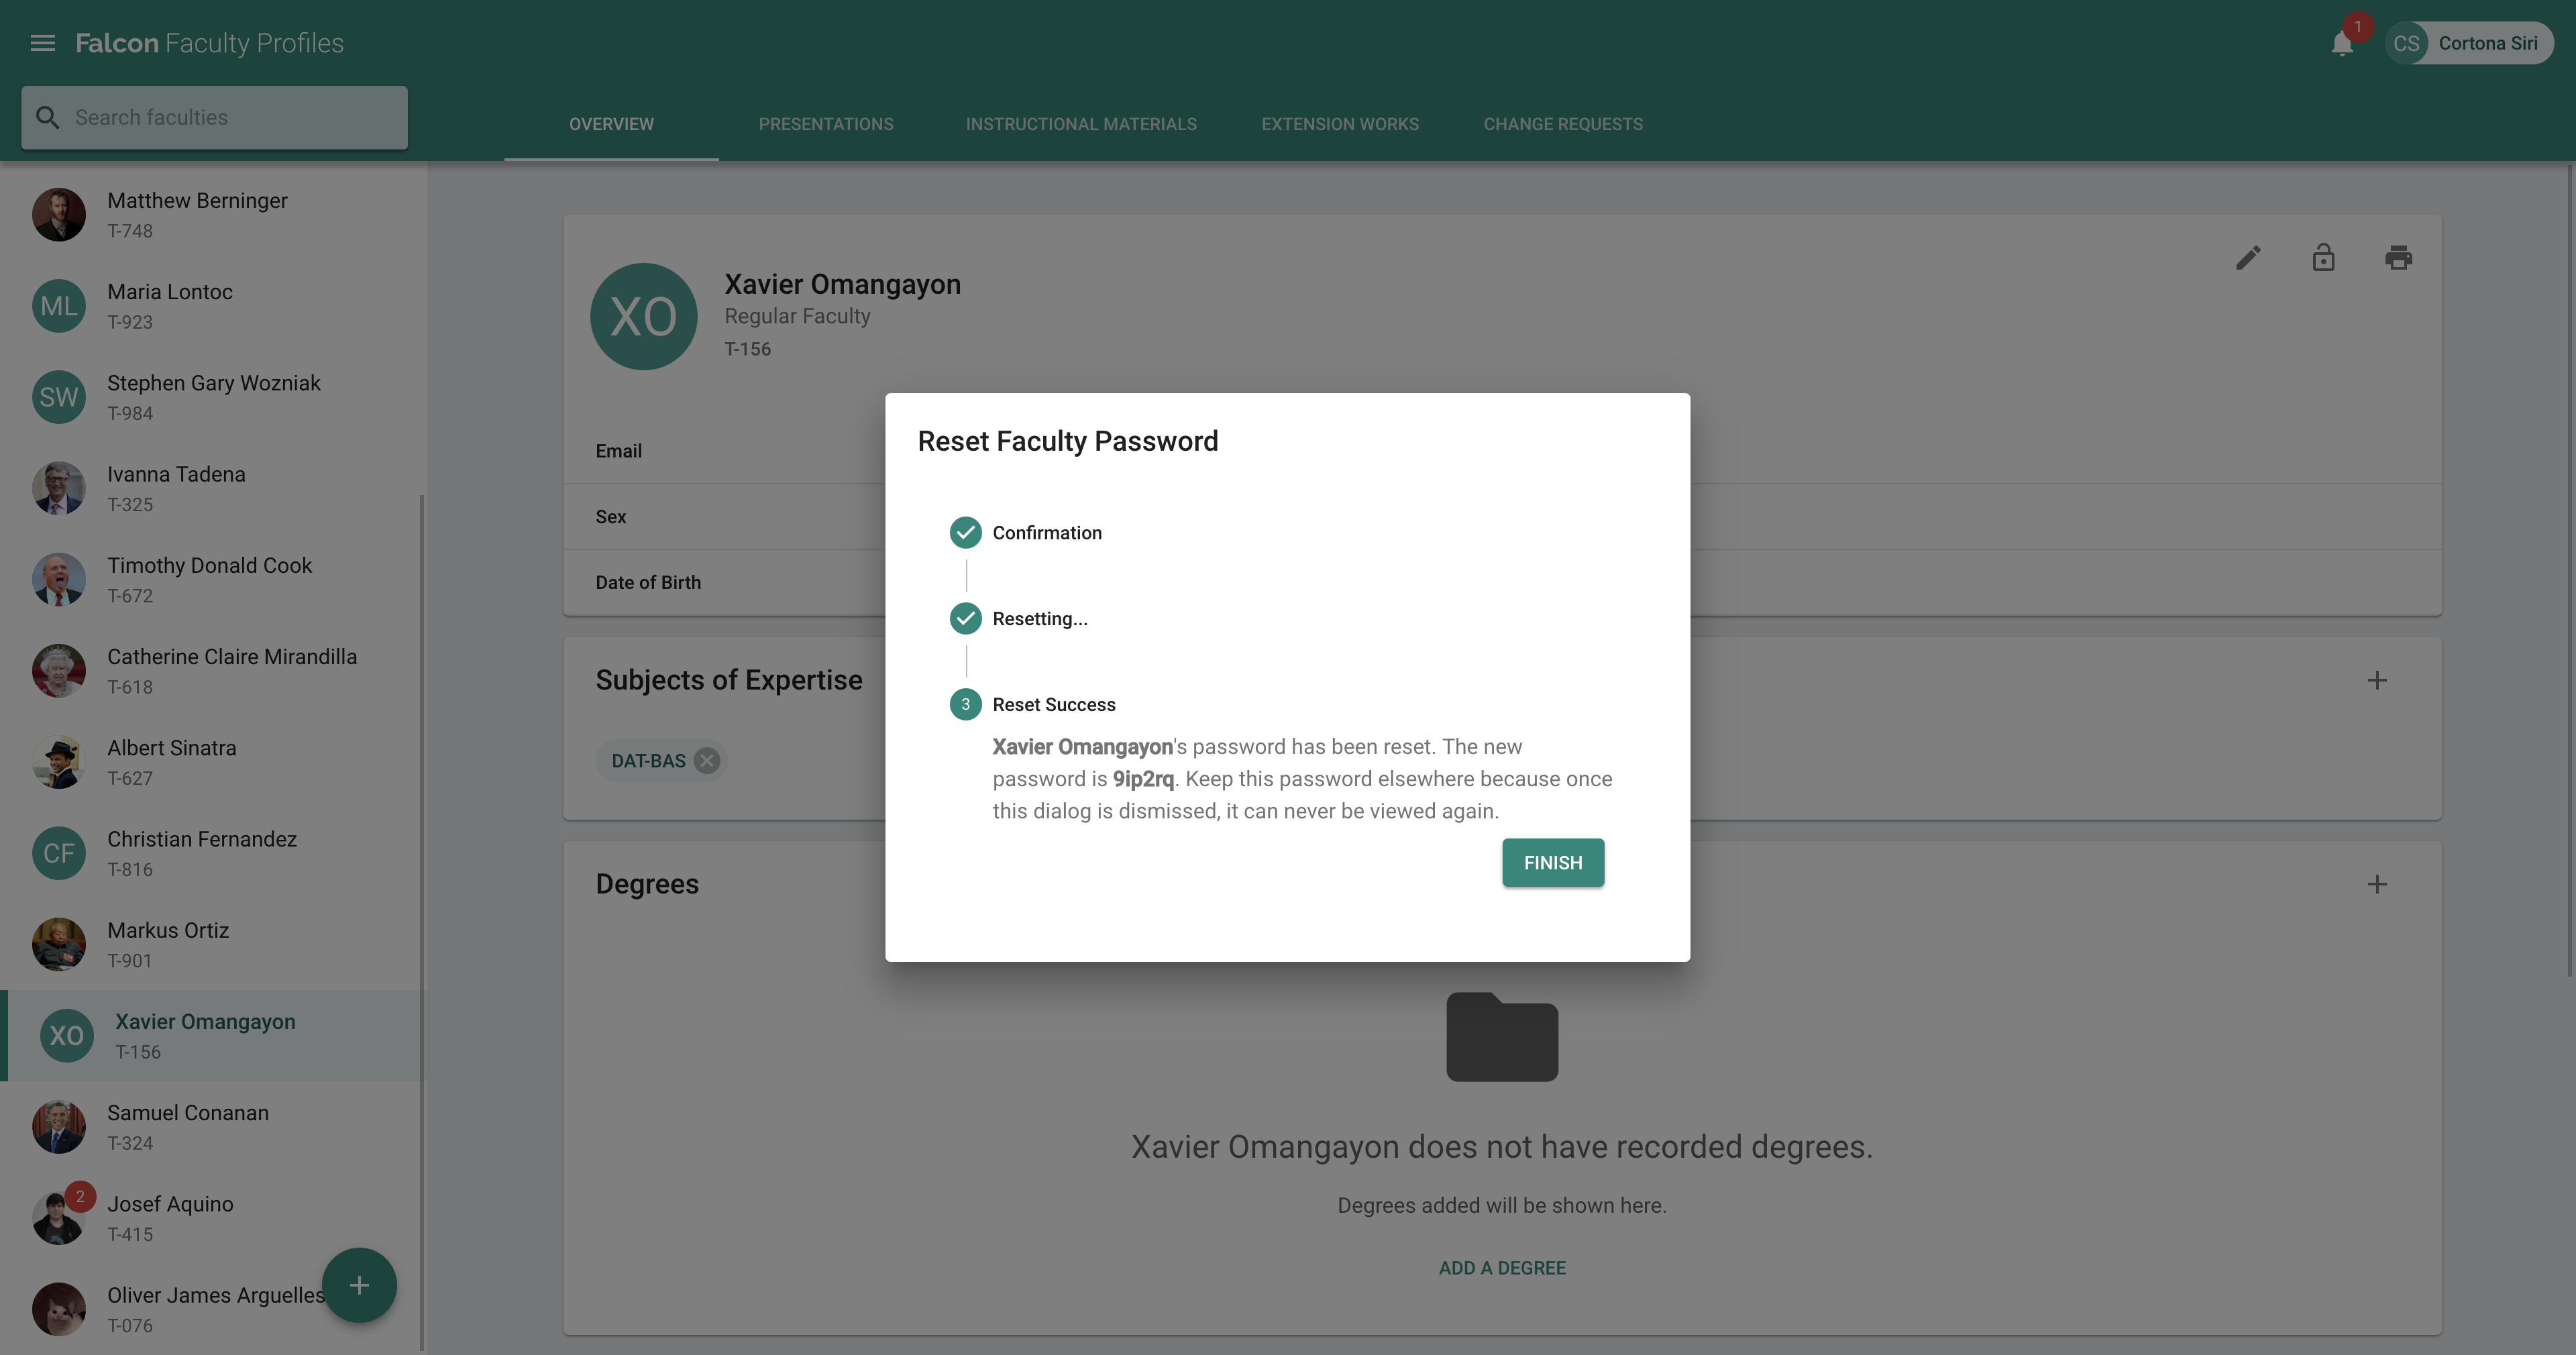
\includegraphics[width=\linewidth]{figures/screen_specifications/reset_password2.png}
   \caption{Reset Password Screen B}
   }
   
   \pagebreak
    
    \subsubsection{Presentations}
    
    \field{Screen Name}{Presentations}
    
    \field{File Name}{$/pages/FacultyProfiles/components/faculty_detail_tabs/PresentationsTab/index.js$}
    
    \field{Description} {Displays the list of presentations of the faculty profile with the details of each presentation, such as the category, date, sponsor, venue, conference, medium, and duration.}
    
    \field{Layout}{}
    
\makefigure{!ht}{
   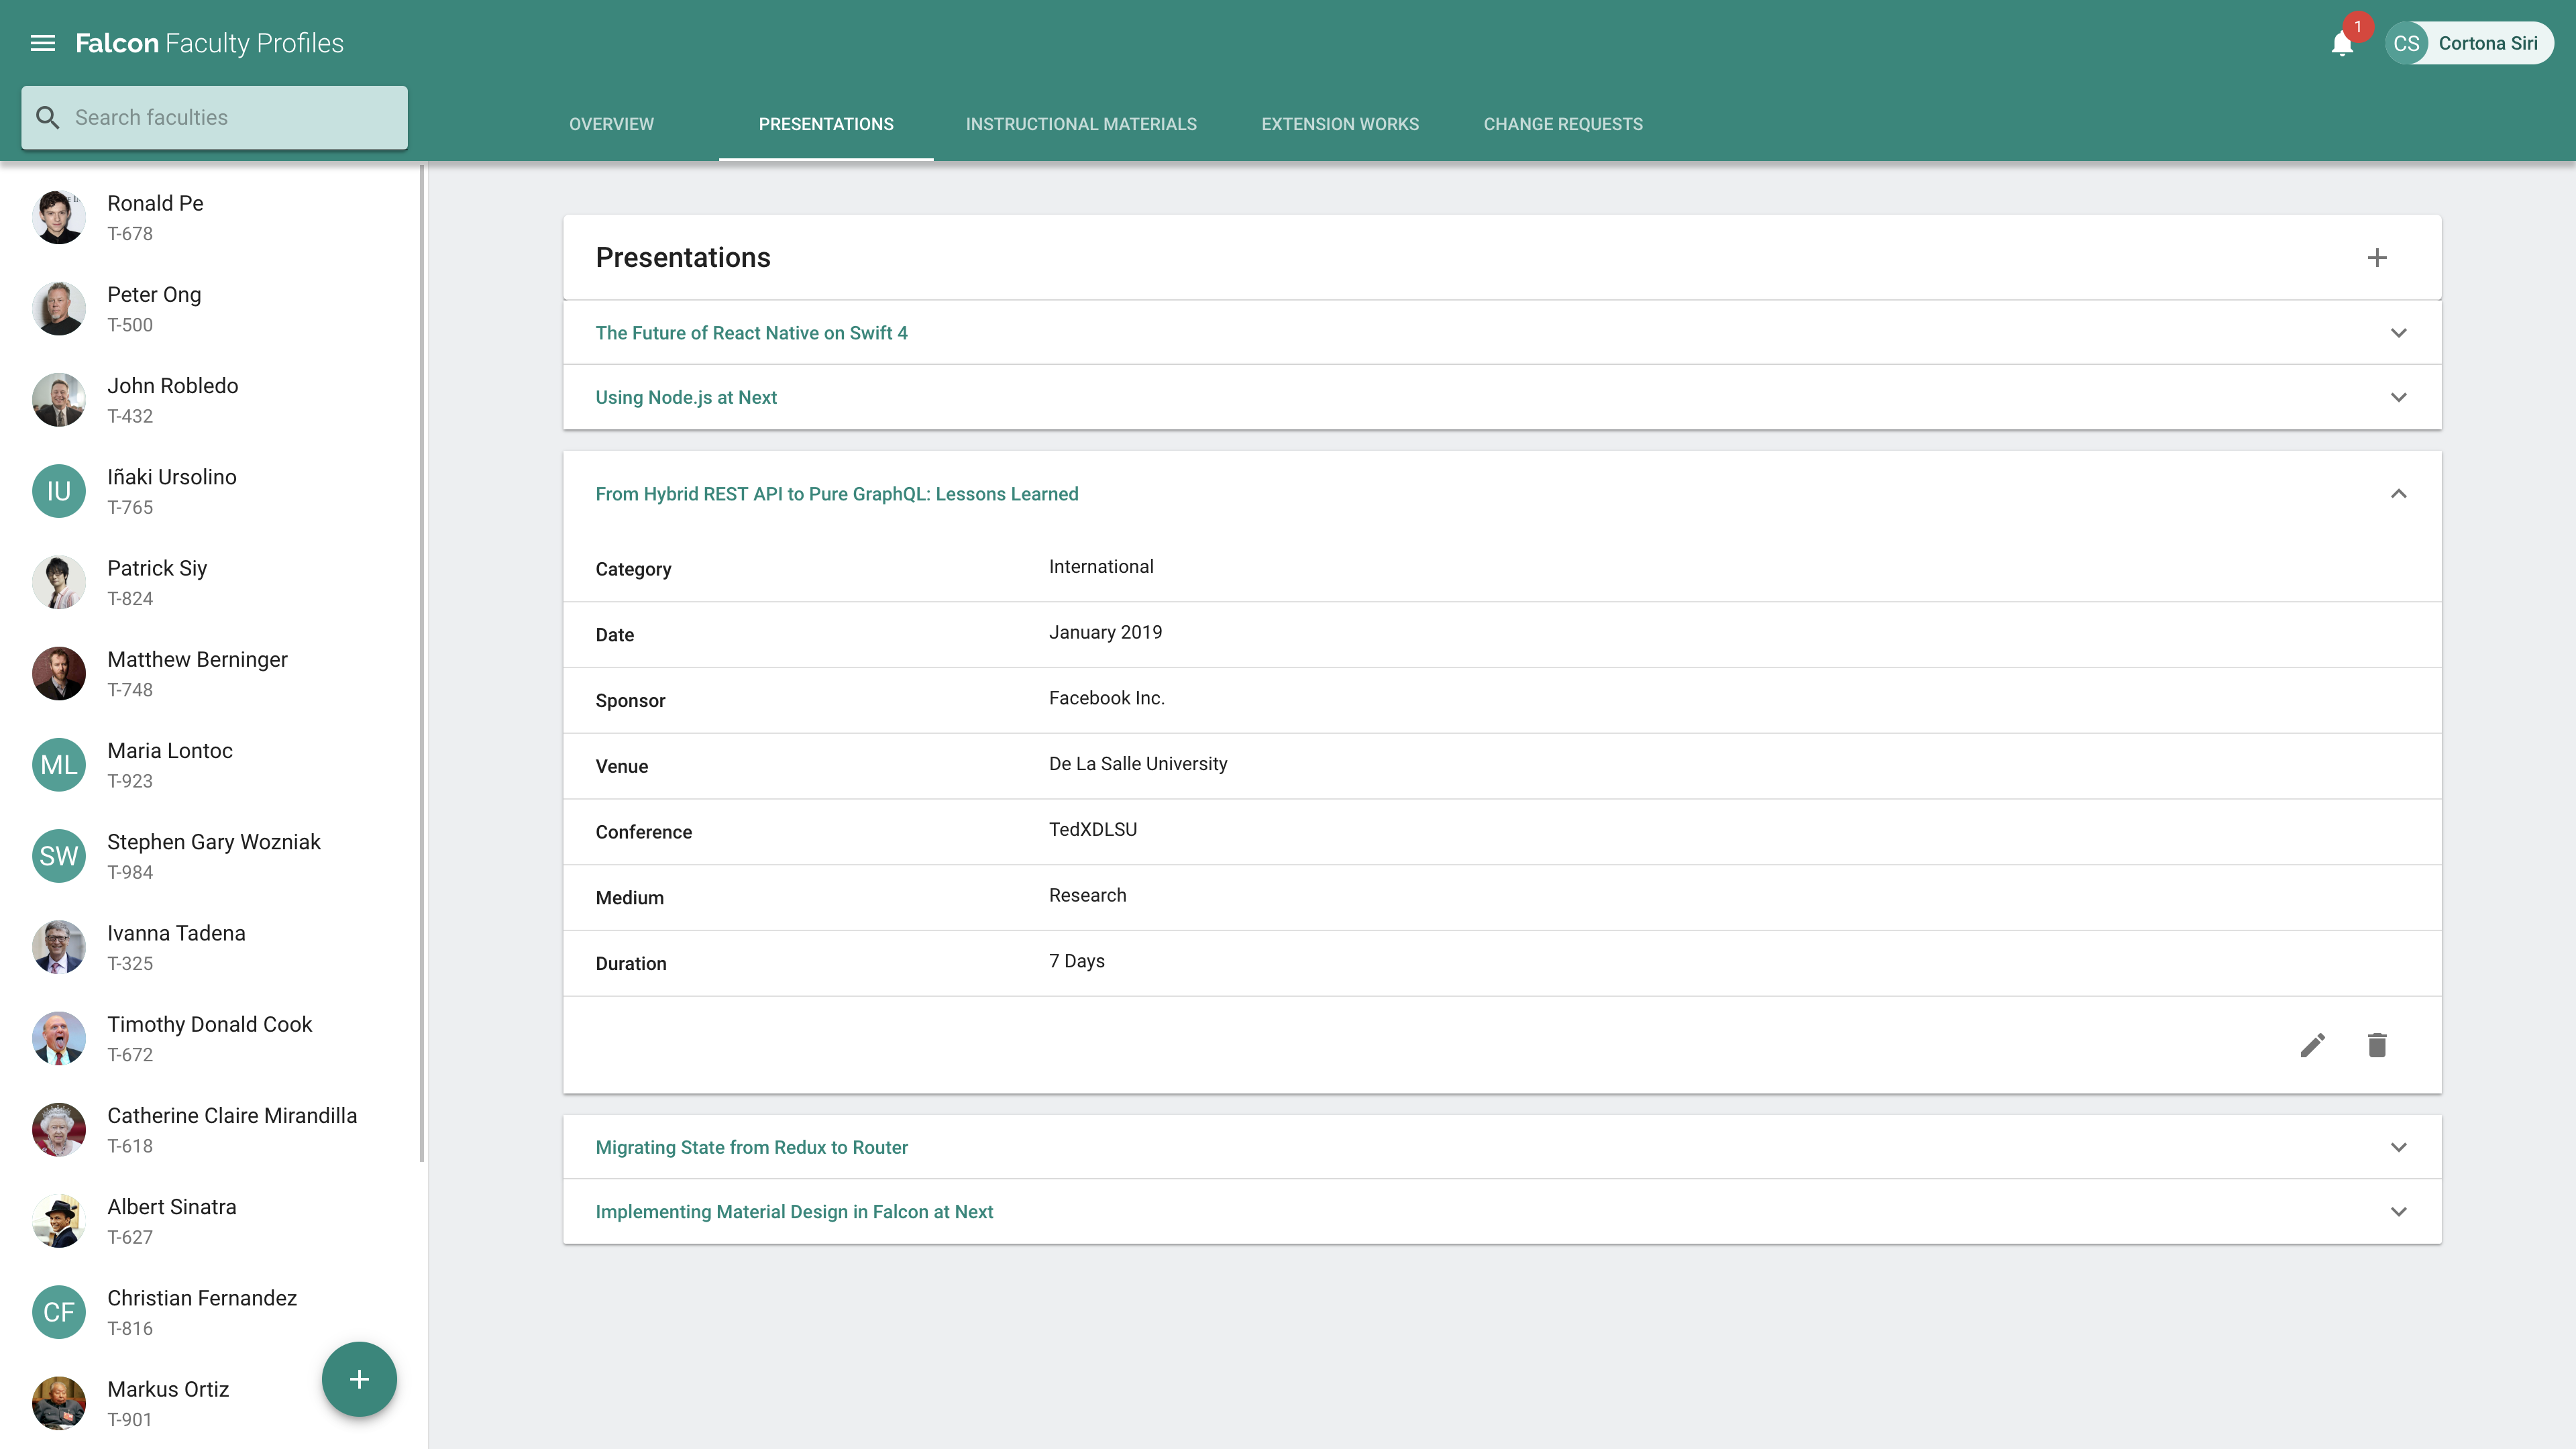
\includegraphics[width=\linewidth]{figures/screen_specifications/presentations.png}
   \caption{Presentations Screen}
   }
   
   \pagebreak
   
   \subsubsection{Remove Presentations}
    
    \field{Screen Name}{Remove Presentations}
    
    \field{File Name}{$/pages/FacultyProfiles/components/modals/RemovePresentationModal/index.js$}
    
    \field{Description} {To confirm the removal of the presentations on the faculty profile by the clerk or dean.}
    
    \field{Layout}{}
    
\makefigure{!ht}{
   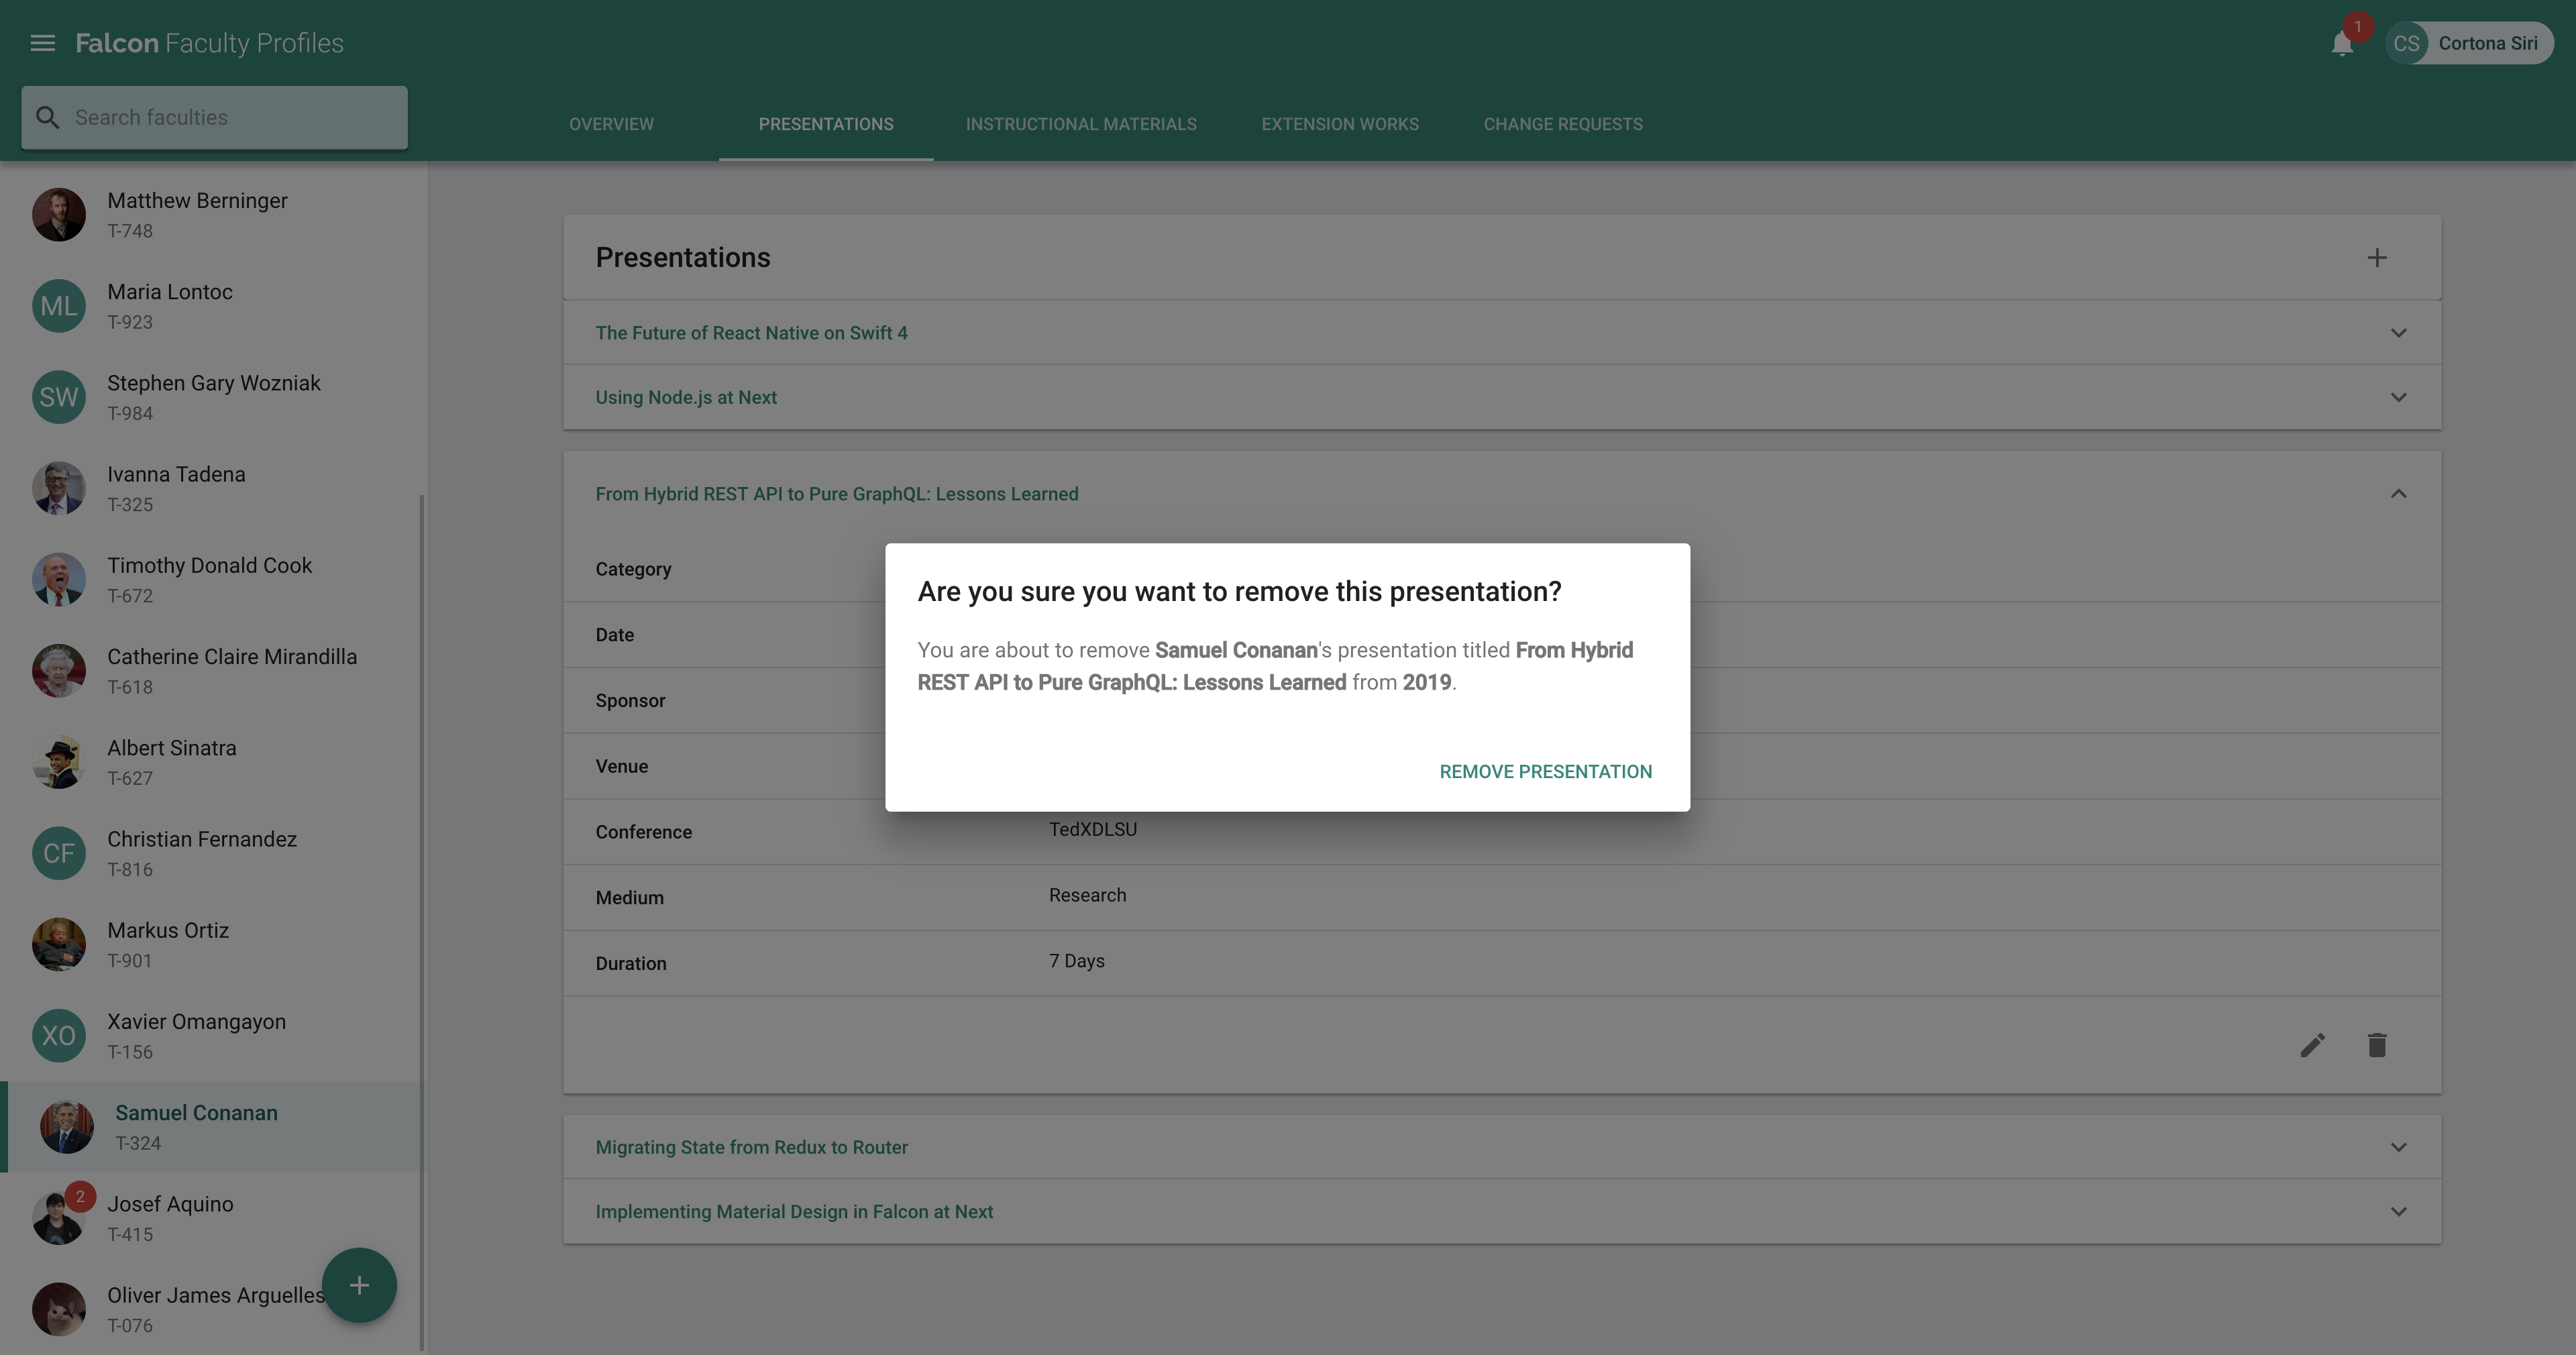
\includegraphics[width=\linewidth]{figures/screen_specifications/remove_presentation.png}
   \caption{Remove Presentations Screen}
   }
   
   \pagebreak
   
    
    \subsubsection{Instructional Materials}
    \field{Screen Name}{Instructional Materials}
    
    \field{File Name}{$/pages/FacultyProfiles/components/faculty_detail_tabs/InstructionalMaterialsTab/index.js$}

    \field{Description}{Displays the list of instructional materials of the faculty member and details of each instructional material. Details include the medium, audience, usage year, and student level.}
    
    \field{Layout}{}
    
\makefigure{!ht}{
   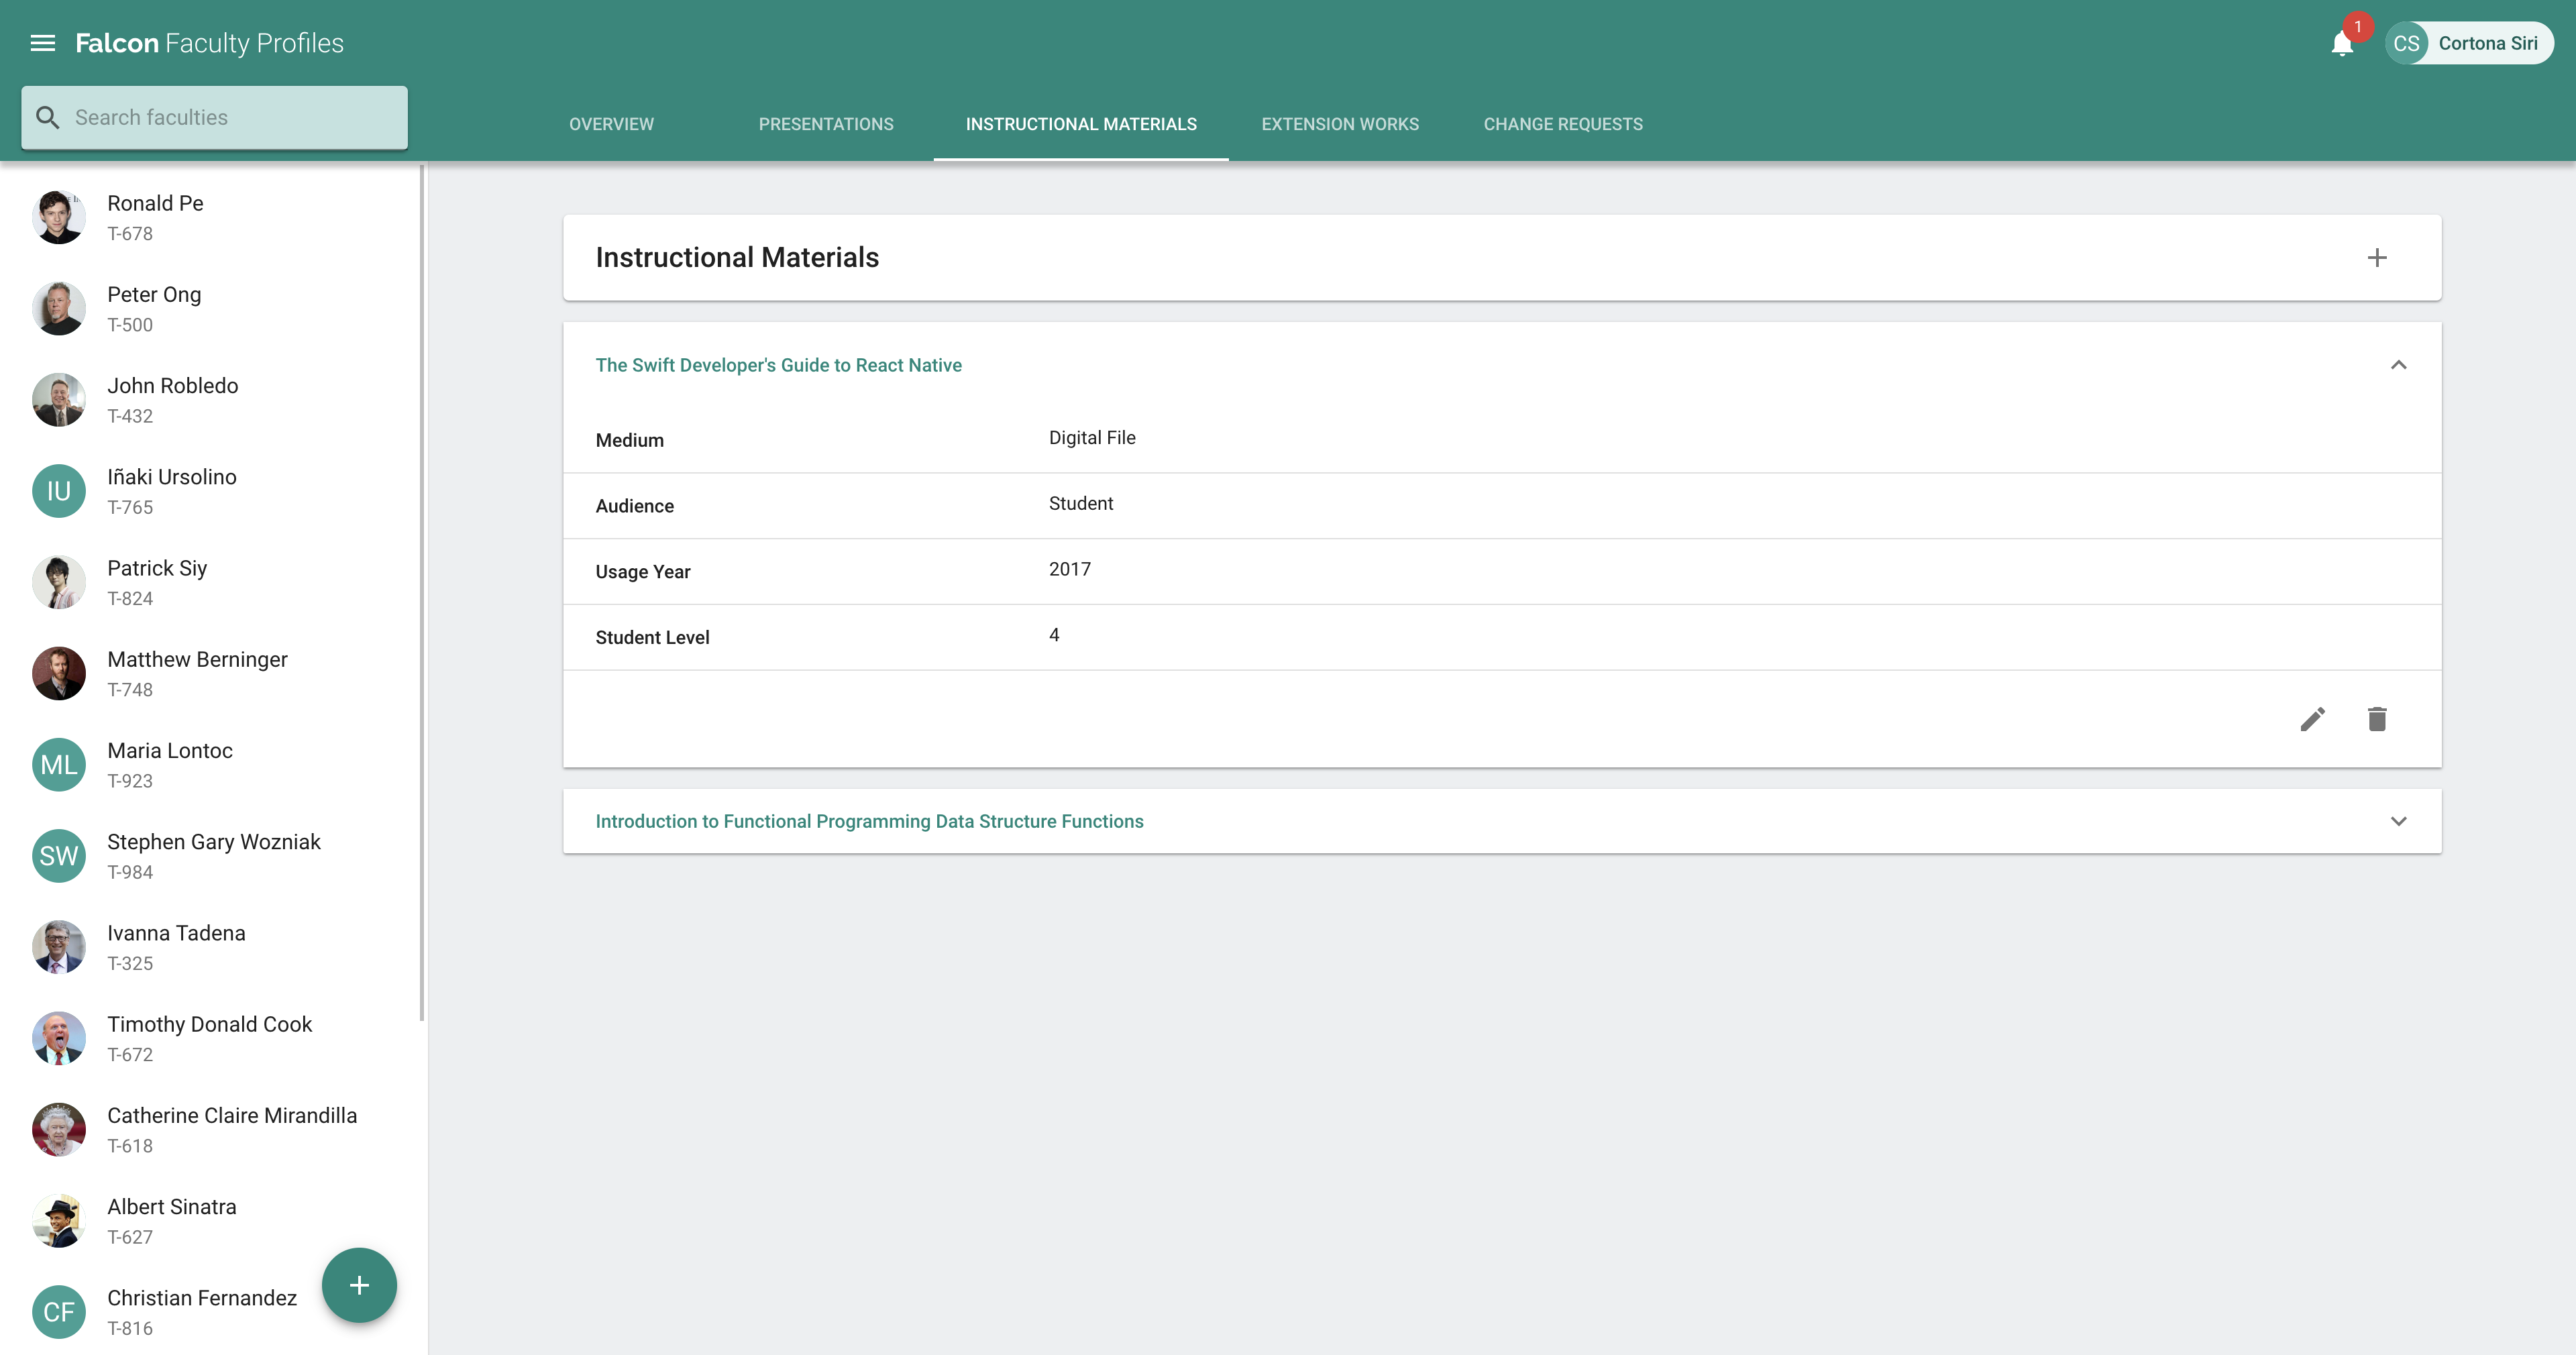
\includegraphics[width=\linewidth]{figures/screen_specifications/instructional_materials.png}
   \caption{Instructional Materials Screen}
   }
    \pagebreak

\subsubsection{Remove Instructional Materials}
    \field{Screen Name}{Remove Instructional Materials}
    
    \field{File Name}{$/pages/FacultyProfiles/components/modals/RemoveInstructionalMaterialModal/index.js$}

    \field{Description}{Confirm the clerk or dean if they want to remove the instructional material from the faculty profile.}
    
    \field{Layout}{}
    
\makefigure{!ht}{
   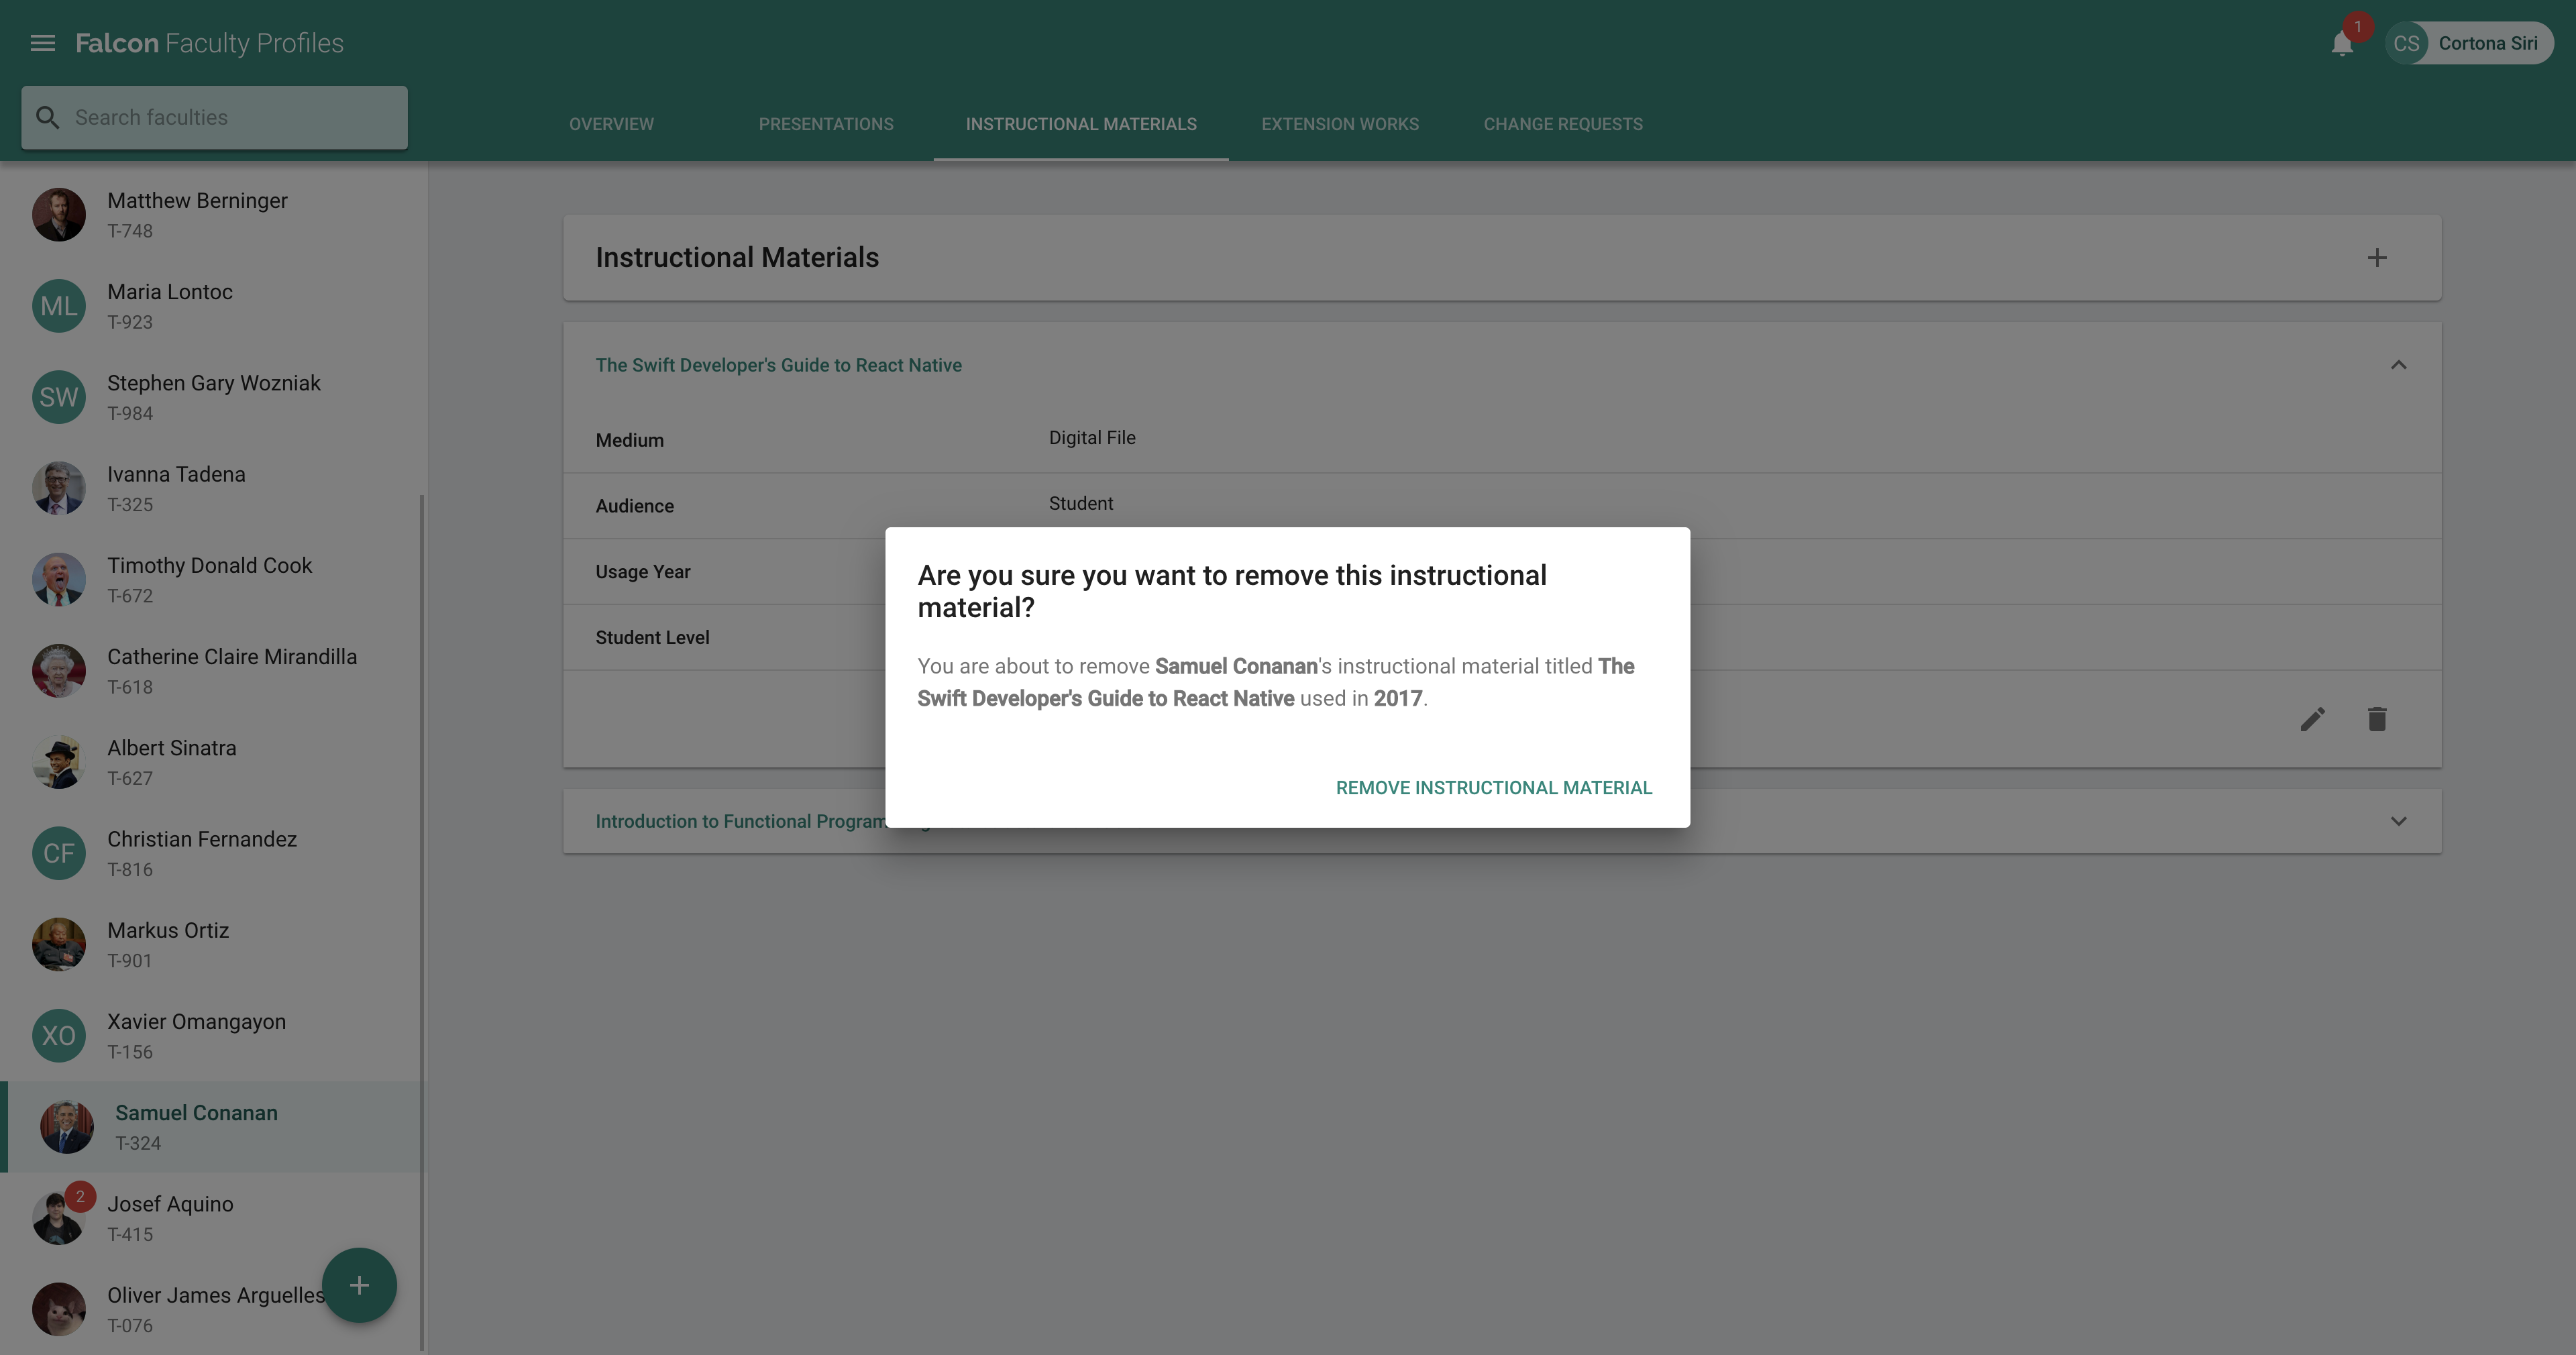
\includegraphics[width=\linewidth]{figures/screen_specifications/remove_instructional.png}
   \caption{Remove Instructional Materials Screen}
   }
    \pagebreak

    \subsubsection{Extension Works}
    \field{Screen Name}{Extension Works}
    
    \field{File Name}{$/pages/FacultyProfiles/components/faculty_detail_tabs/ExtensionWorksTab/index.js$}
    
    \field{Description}{Displays the list of extension works for the faculty profile with the details of each extension work. The details include the venue and roles.}
    
    \field{Layout}{} 
    
\makefigure{!ht}{
   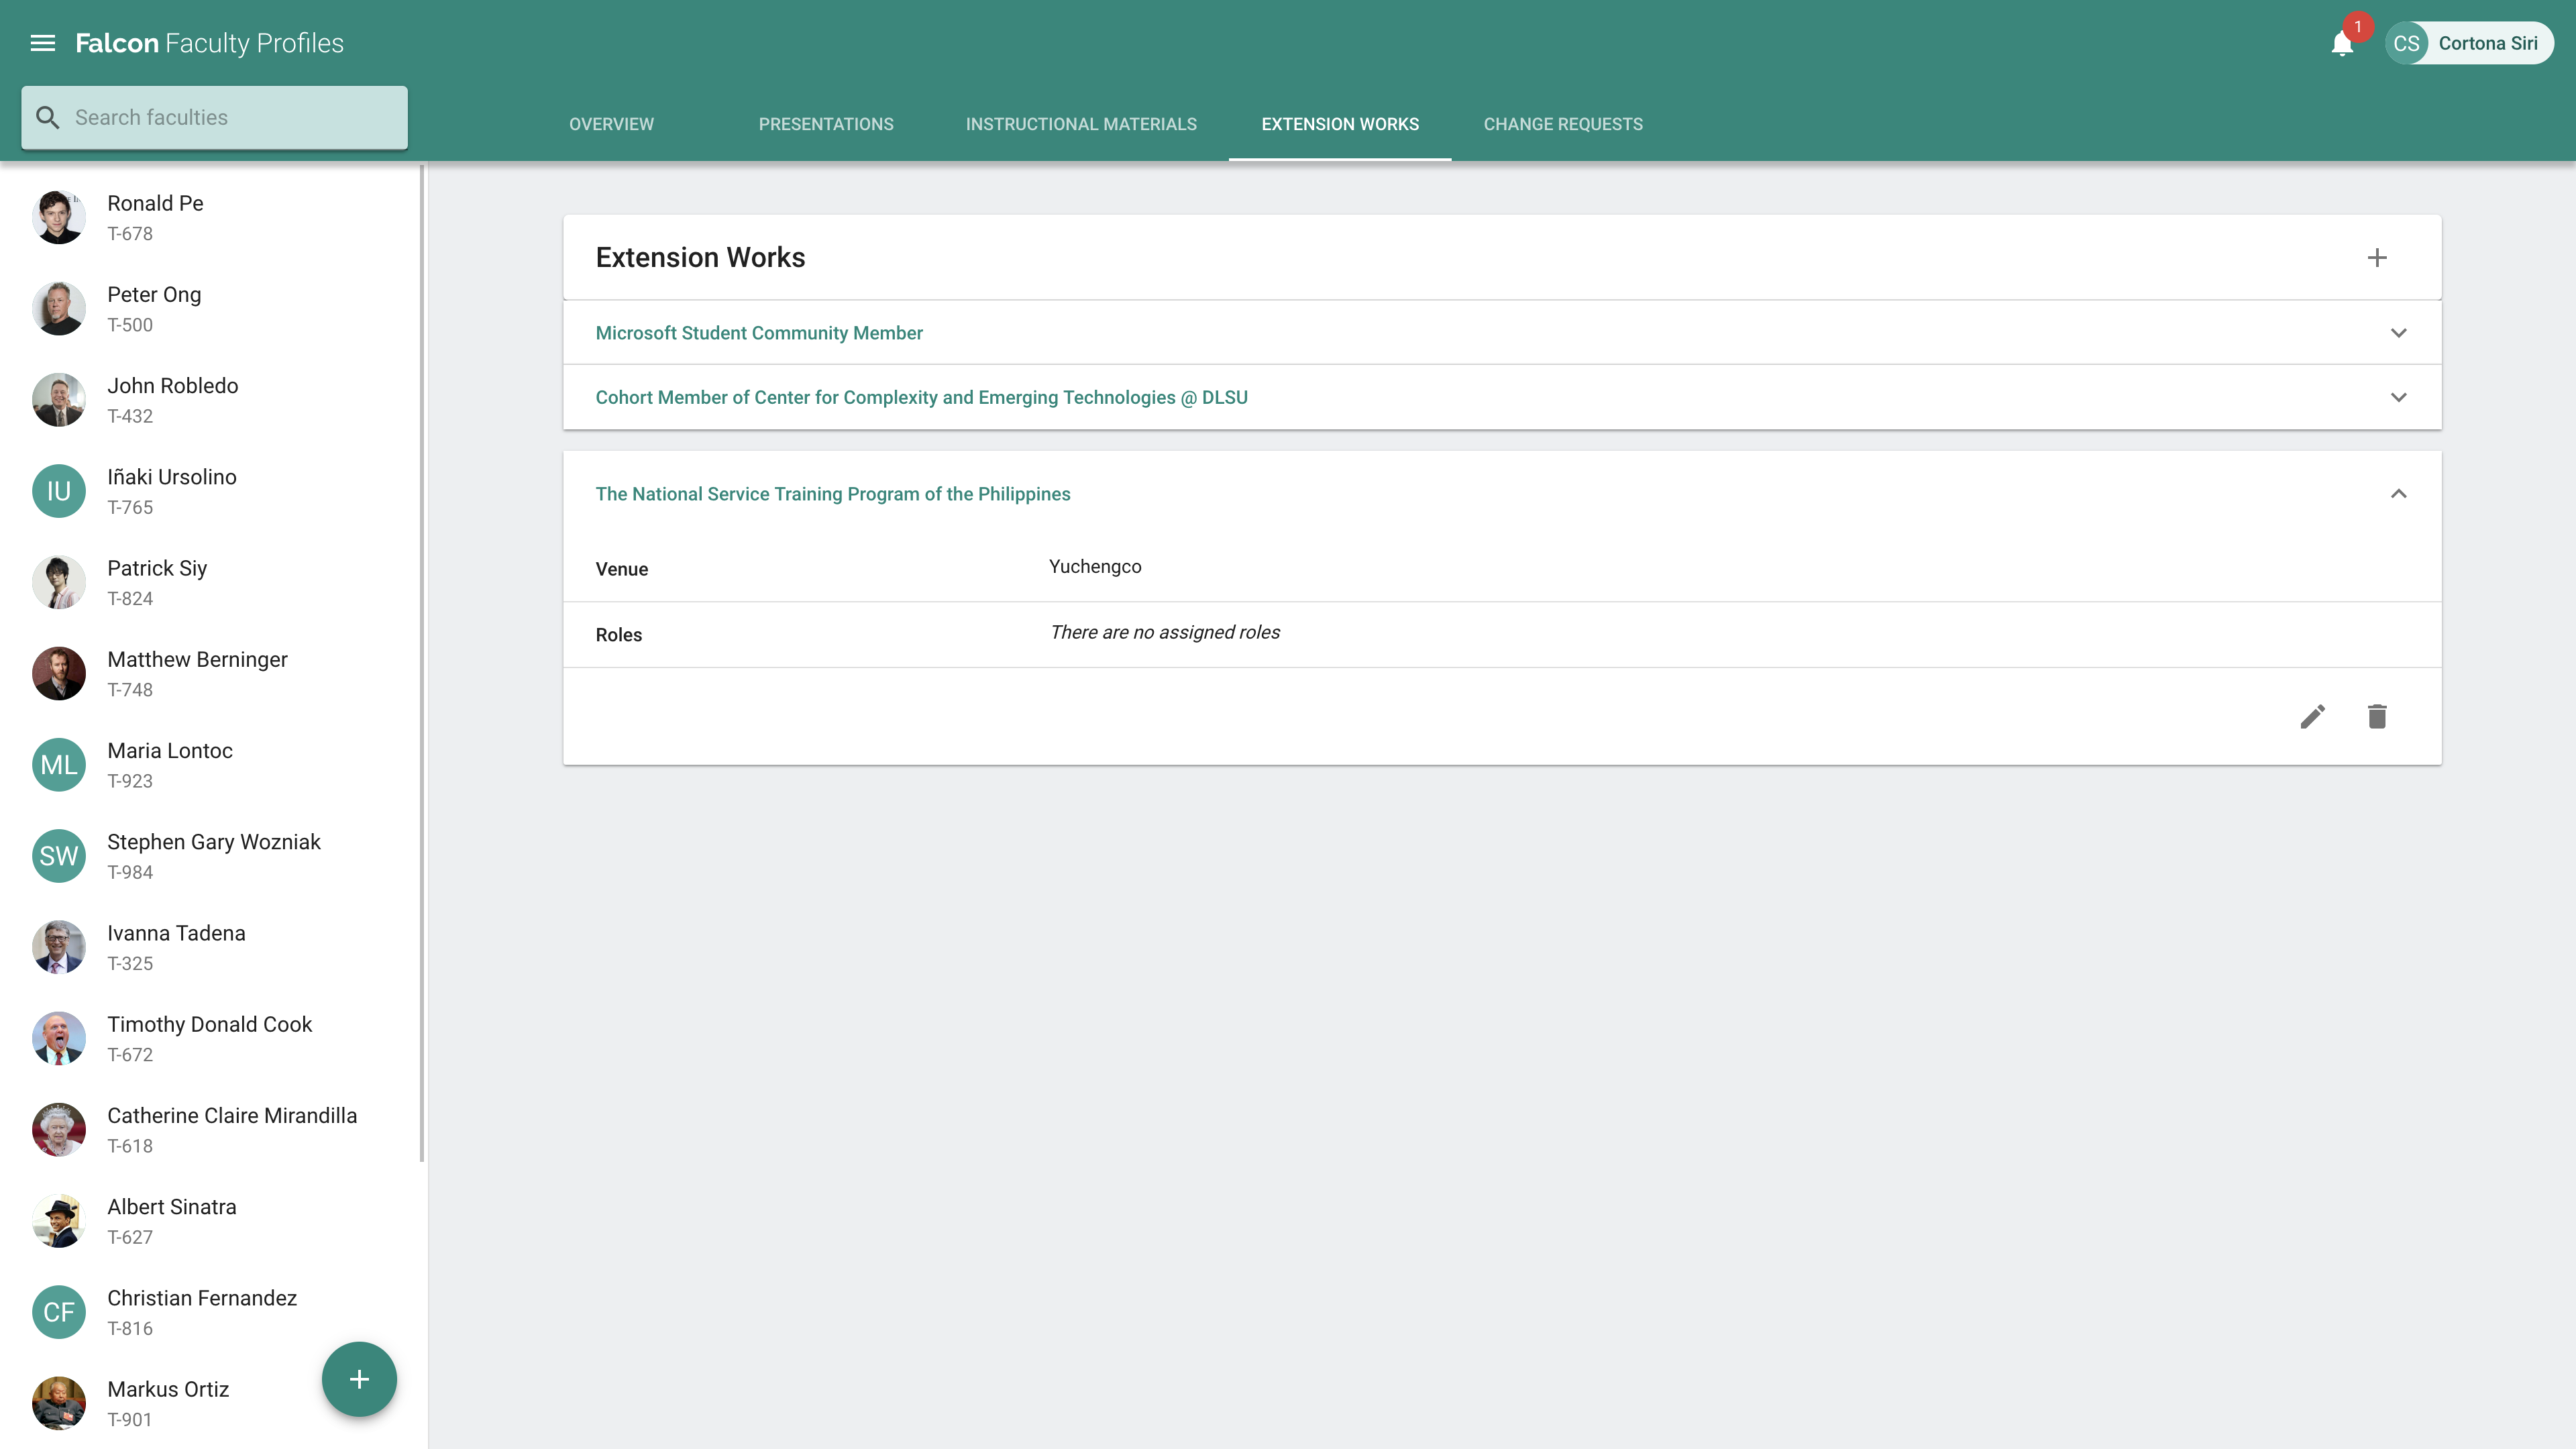
\includegraphics[width=\linewidth]{figures/screen_specifications/extension_works.png}
   \caption{Extension Works Screen}
   }
   \pagebreak
   
   \subsubsection{Remove Extension Works}
    \field{Screen Name}{Remove Extension Works}
    
    \field{File Name}{$/pages/FacultyProfiles/components/modals/RemoveExtensionWorkModal/index.js$}
    
    \field{Description}{To confirm the removal of an extension work from the faculty profile by the clerk or dean.}
    
    \field{Layout}{} 
    
\makefigure{!ht}{
   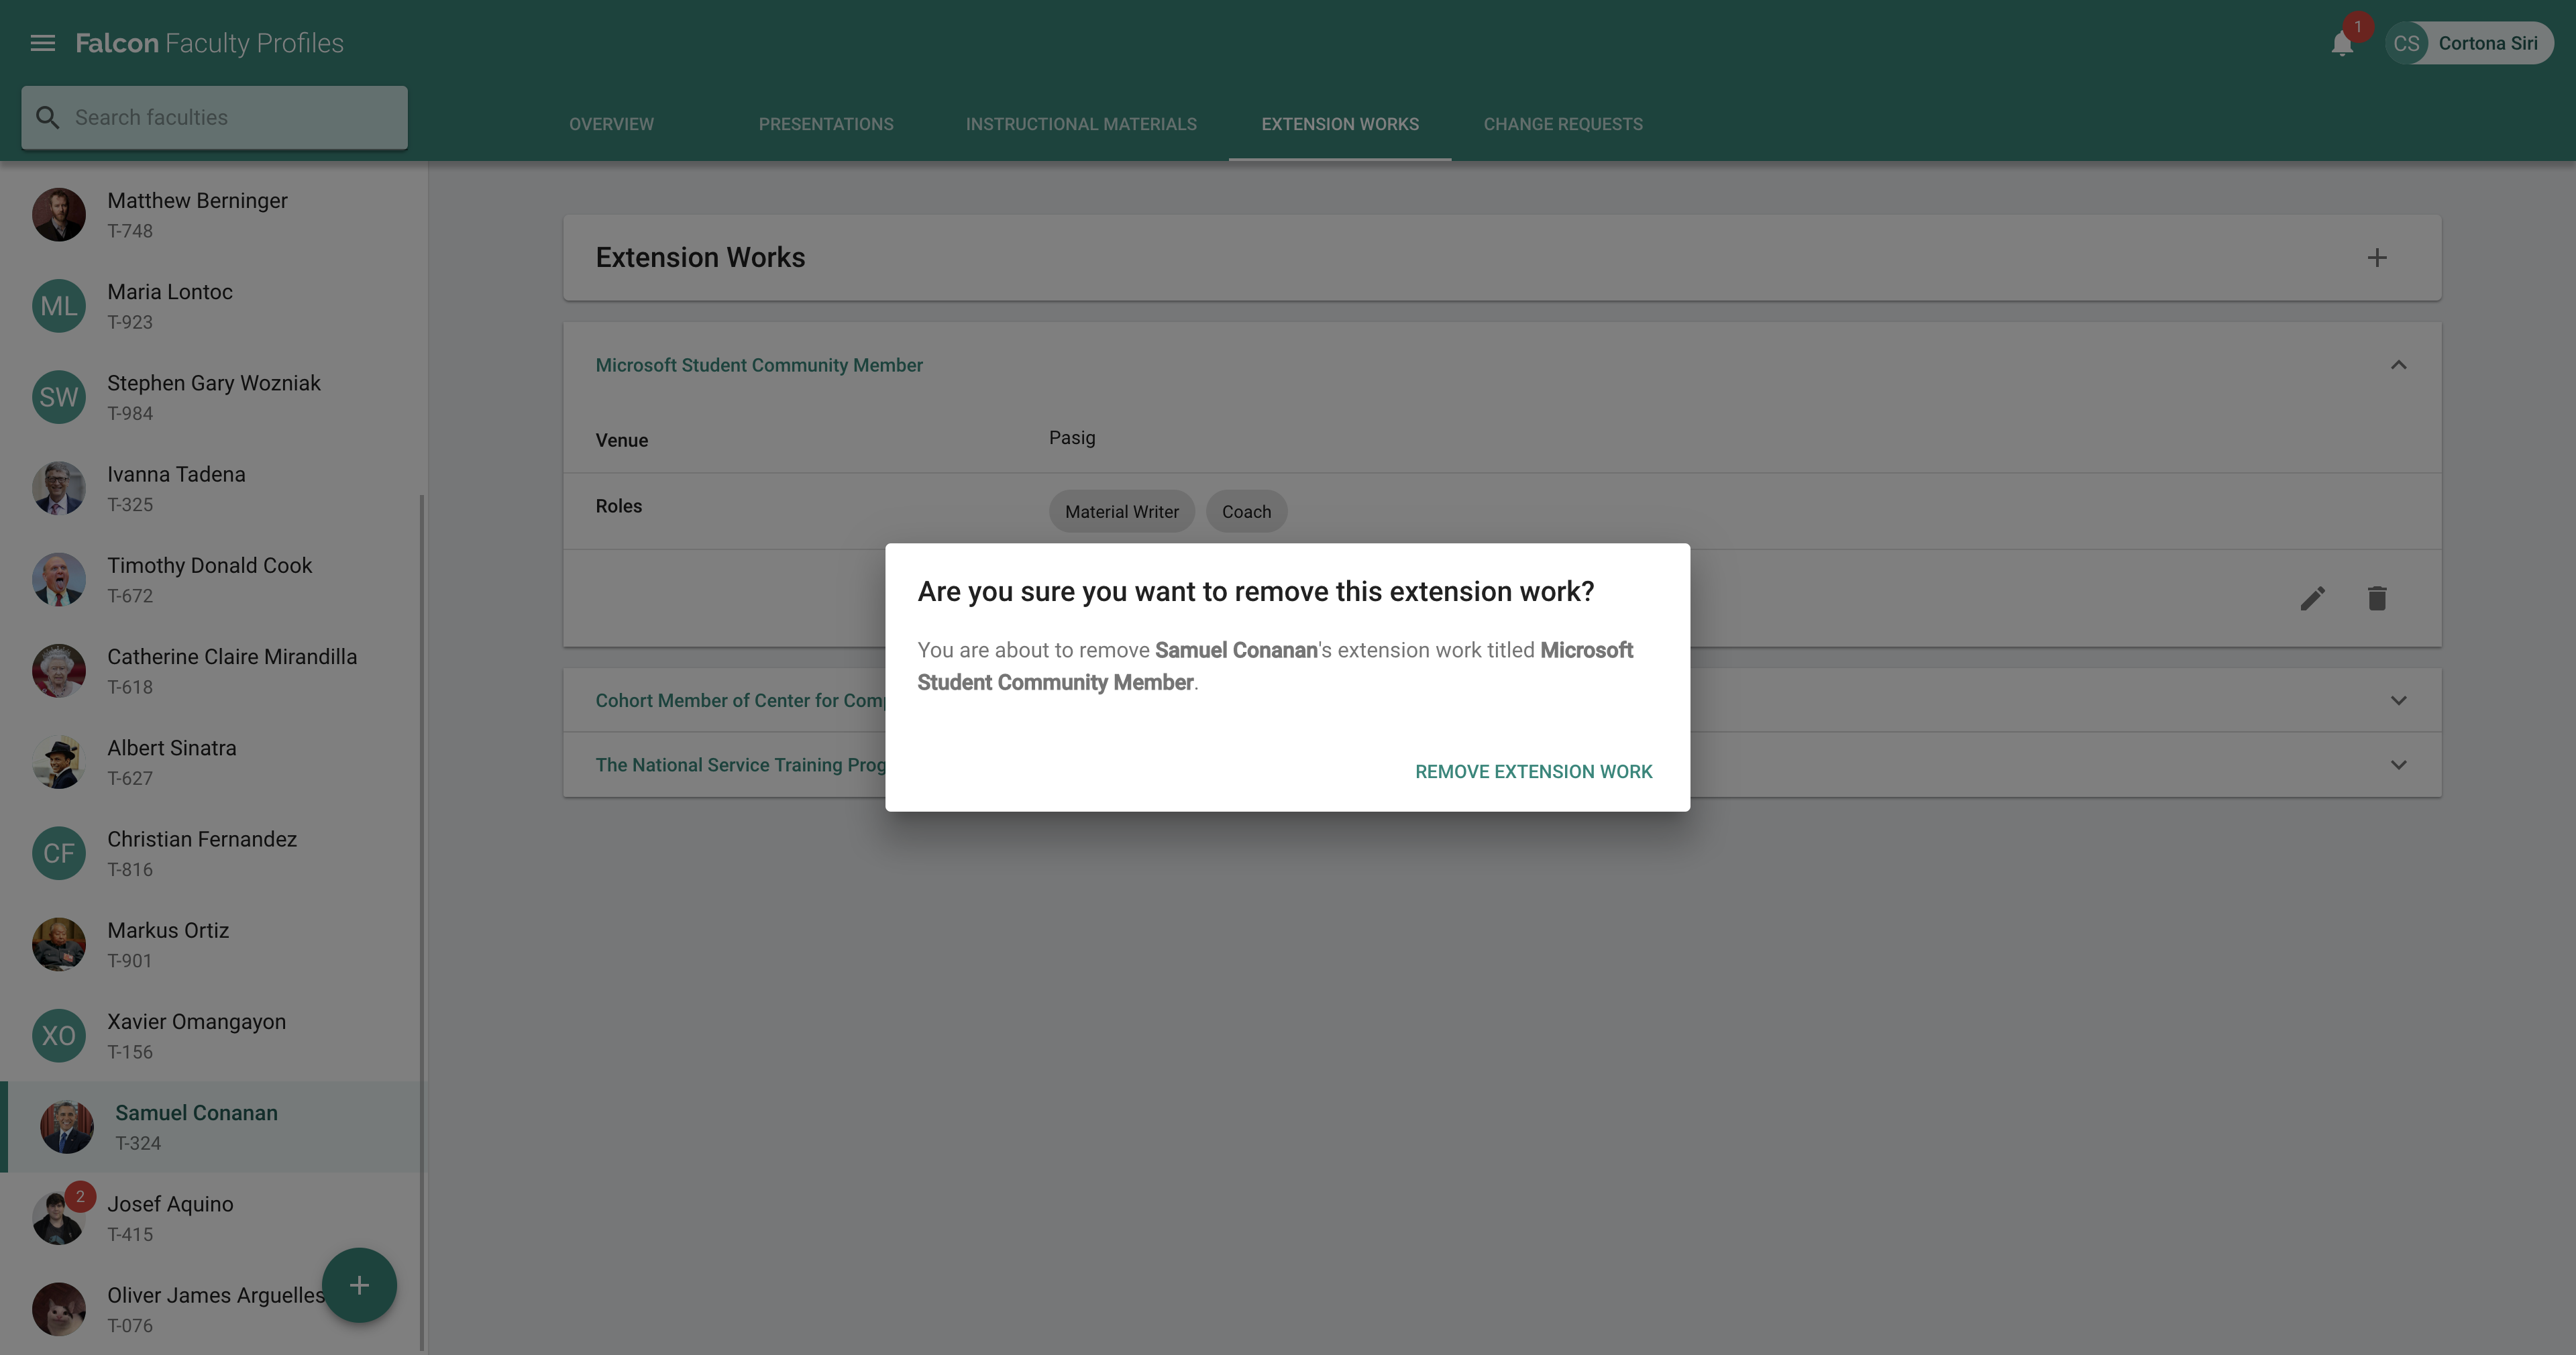
\includegraphics[width=\linewidth]{figures/screen_specifications/remove_extension.png}
   \caption{Remove Extension Works Screen}
   }
   \pagebreak
   
    \subsubsection{Notifications}
    
    \field{Screen Name}{Notifications}
    
    \field{File Name}{$/pages/App/components/notifications/NotificationsButton/index.js$}
    
    \field{Description} {Notifies the user of any updates and shows the list of notifications.}
    
    \field{Layout}{}
    
\makefigure{!ht}{
   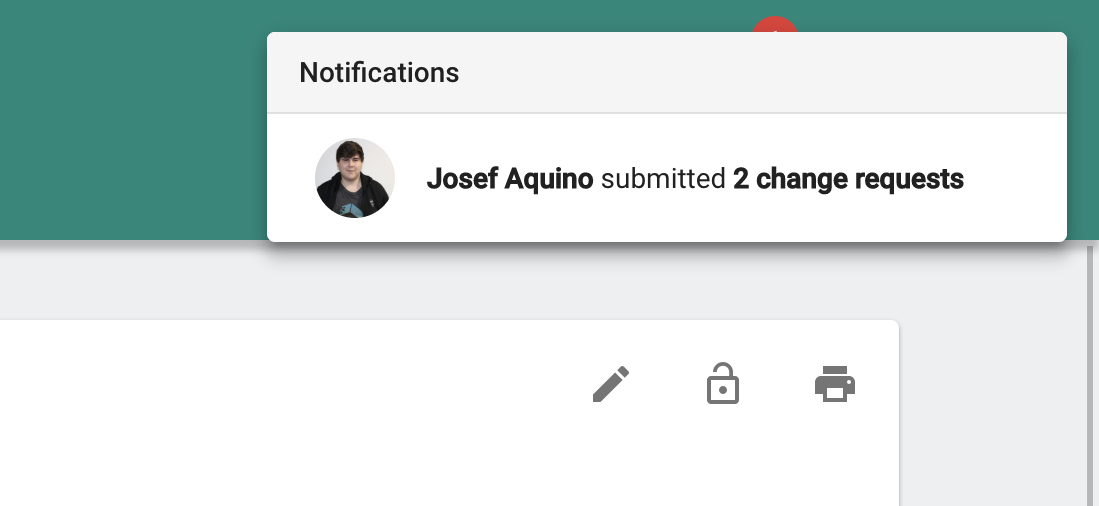
\includegraphics[width=\linewidth]{figures/screen_specifications/notifications.png}
   \caption{Notifications Screen}
   }
   
\pagebreak
   
   \subsubsection{Change Requests}
    
    \field{Screen Name}{Change Requests}
    
    \field{File Name}{$/pages/FacultyProfiles/components/faculty_detail_tabs/ChangeRequestsTab/index.js$}
    
    \field{Description} {Displays the list of change requests of the faculty members with details.}
    
    \field{Layout}{}
    
\makefigure{!ht}{
   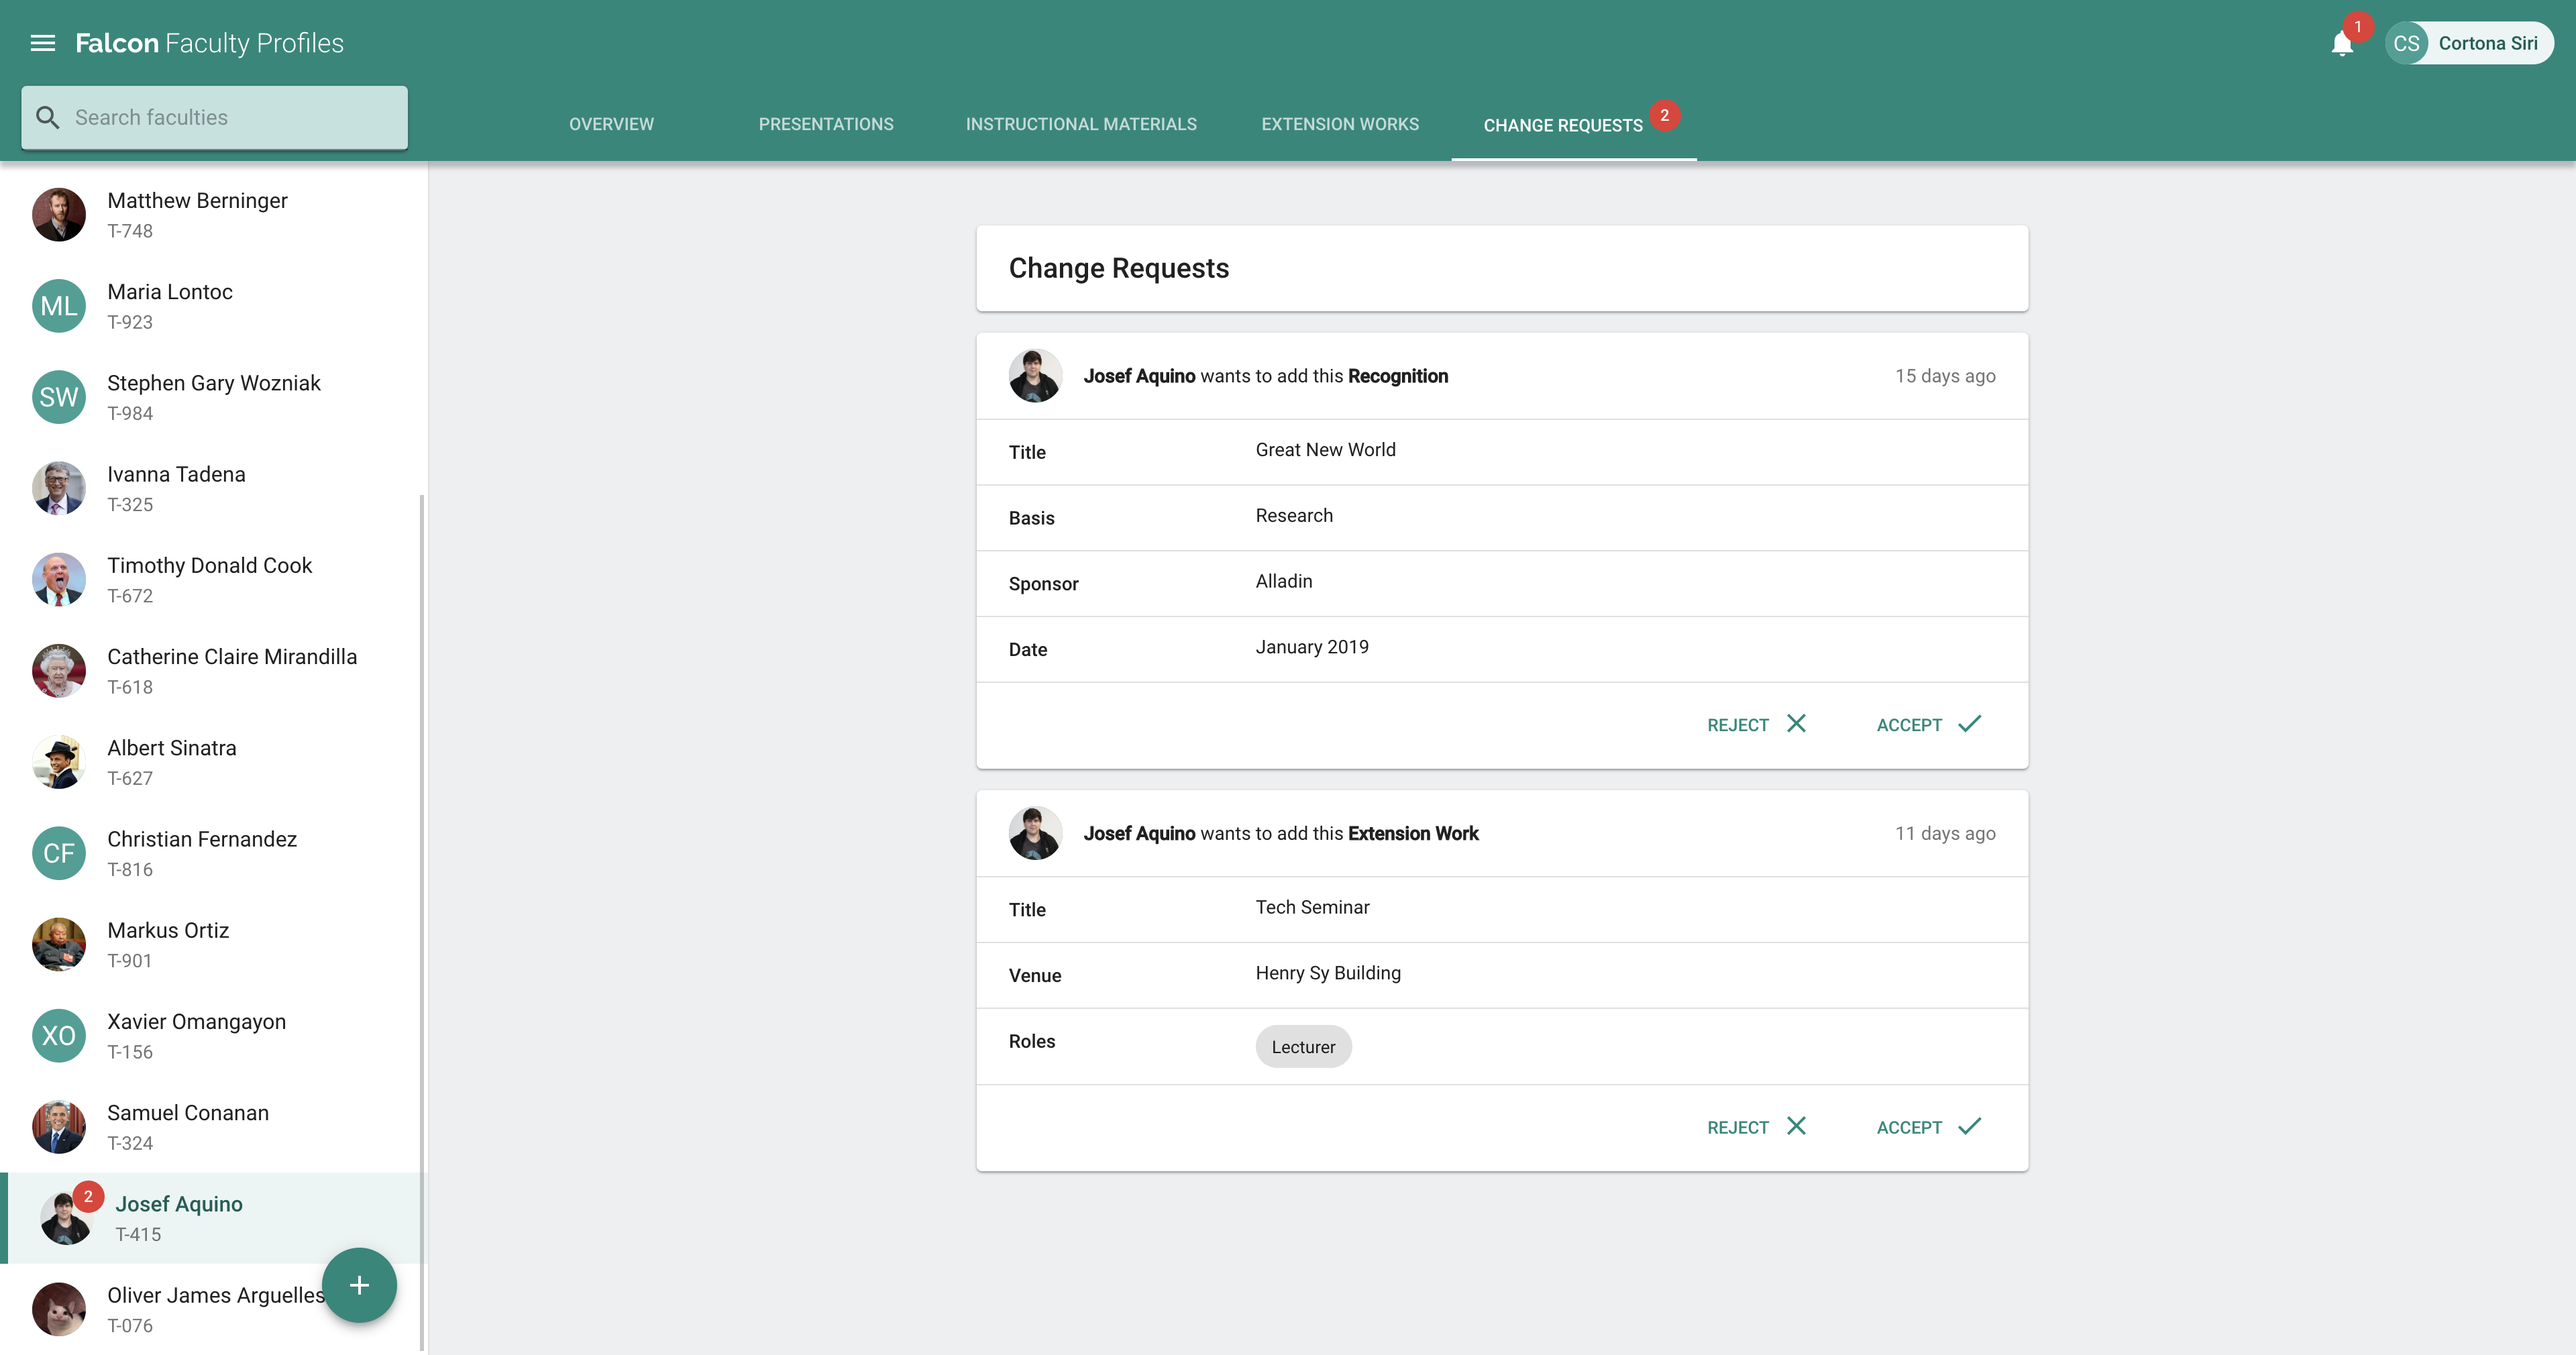
\includegraphics[width=\linewidth]{figures/screen_specifications/change_requests.png}
   \caption{Change Requests Screen}
   }
   
   \pagebreak
   
   \subsection{My Profile}
   
   \subsubsection{My Profile Overview}
    
    \field{Screen Name}{My Profile Overview}
    
    \field{File Name}{$/pages/MyProfile/index.js$}
    
    \field{Description} {Displays the details of the faculty profile. The first card displays the basic information, second displays the expertise of the faculty member, third card displays the degrees, and the fourth displays the recognitions.}
    
    \field{Layout}{}
    
\makefigure{!ht}{
   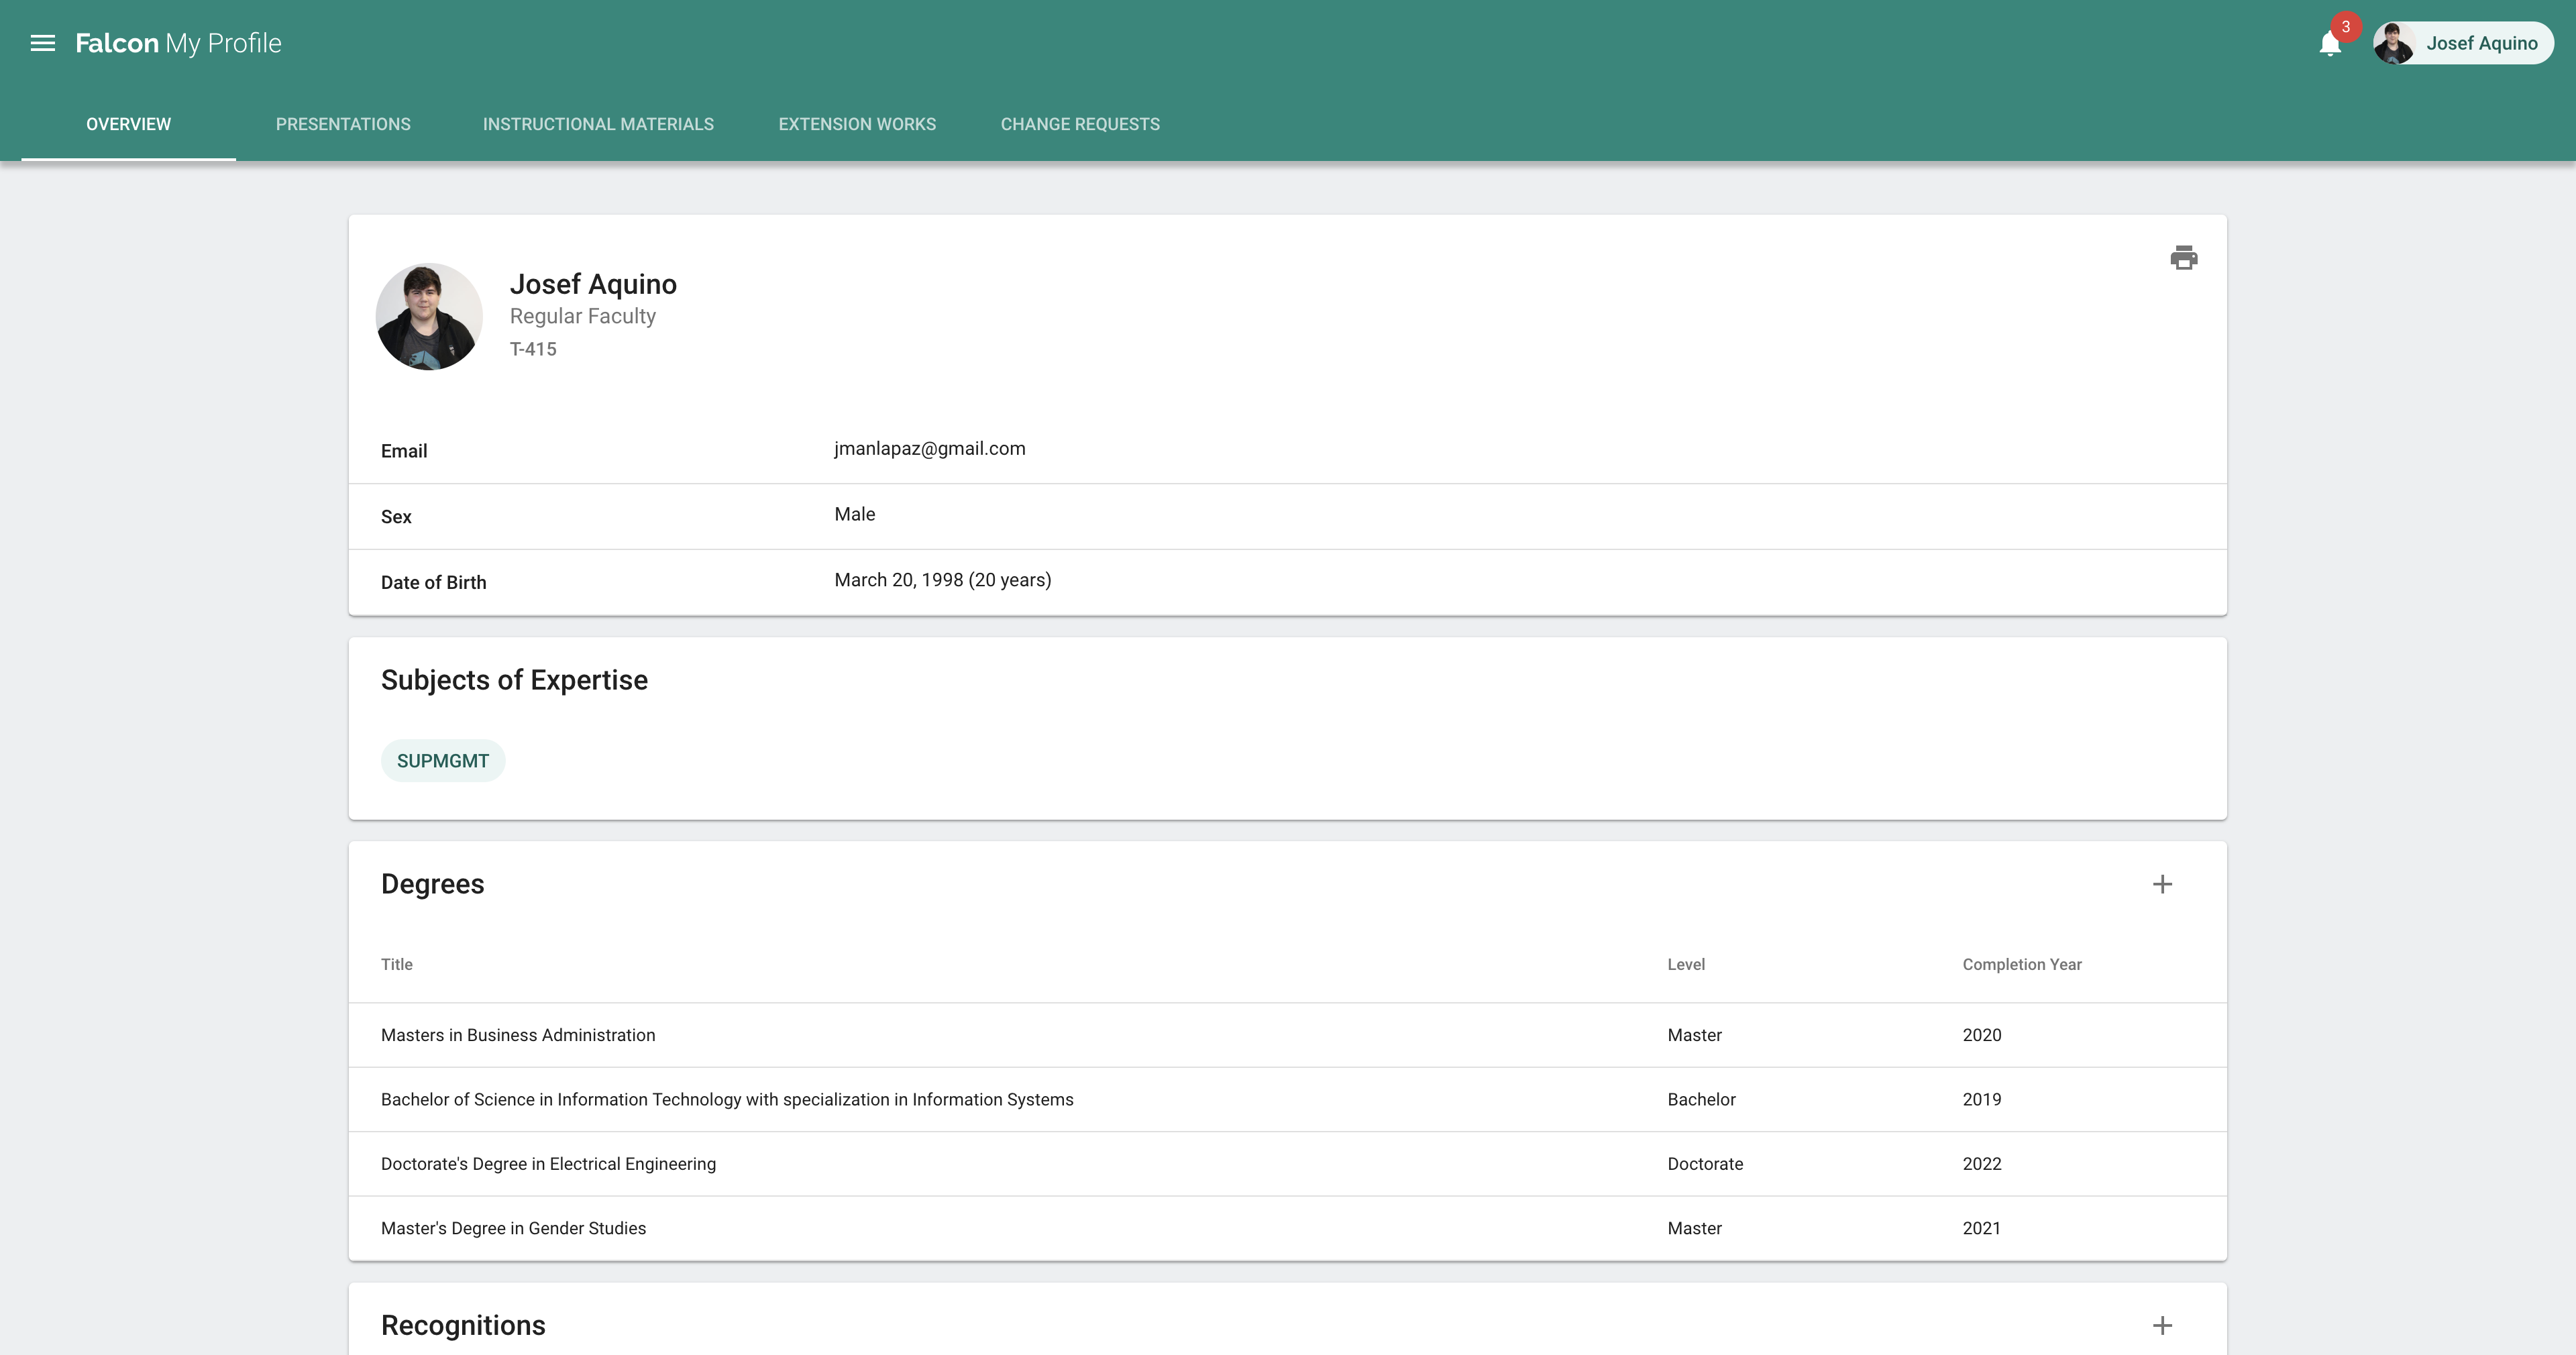
\includegraphics[width=\linewidth]{figures/screen_specifications/myprofile_screens/my_profileA.png}
   \caption{My Profile Overview Screen A}
   }
   
   \pagebreak
   
\makefigure{!ht}{
   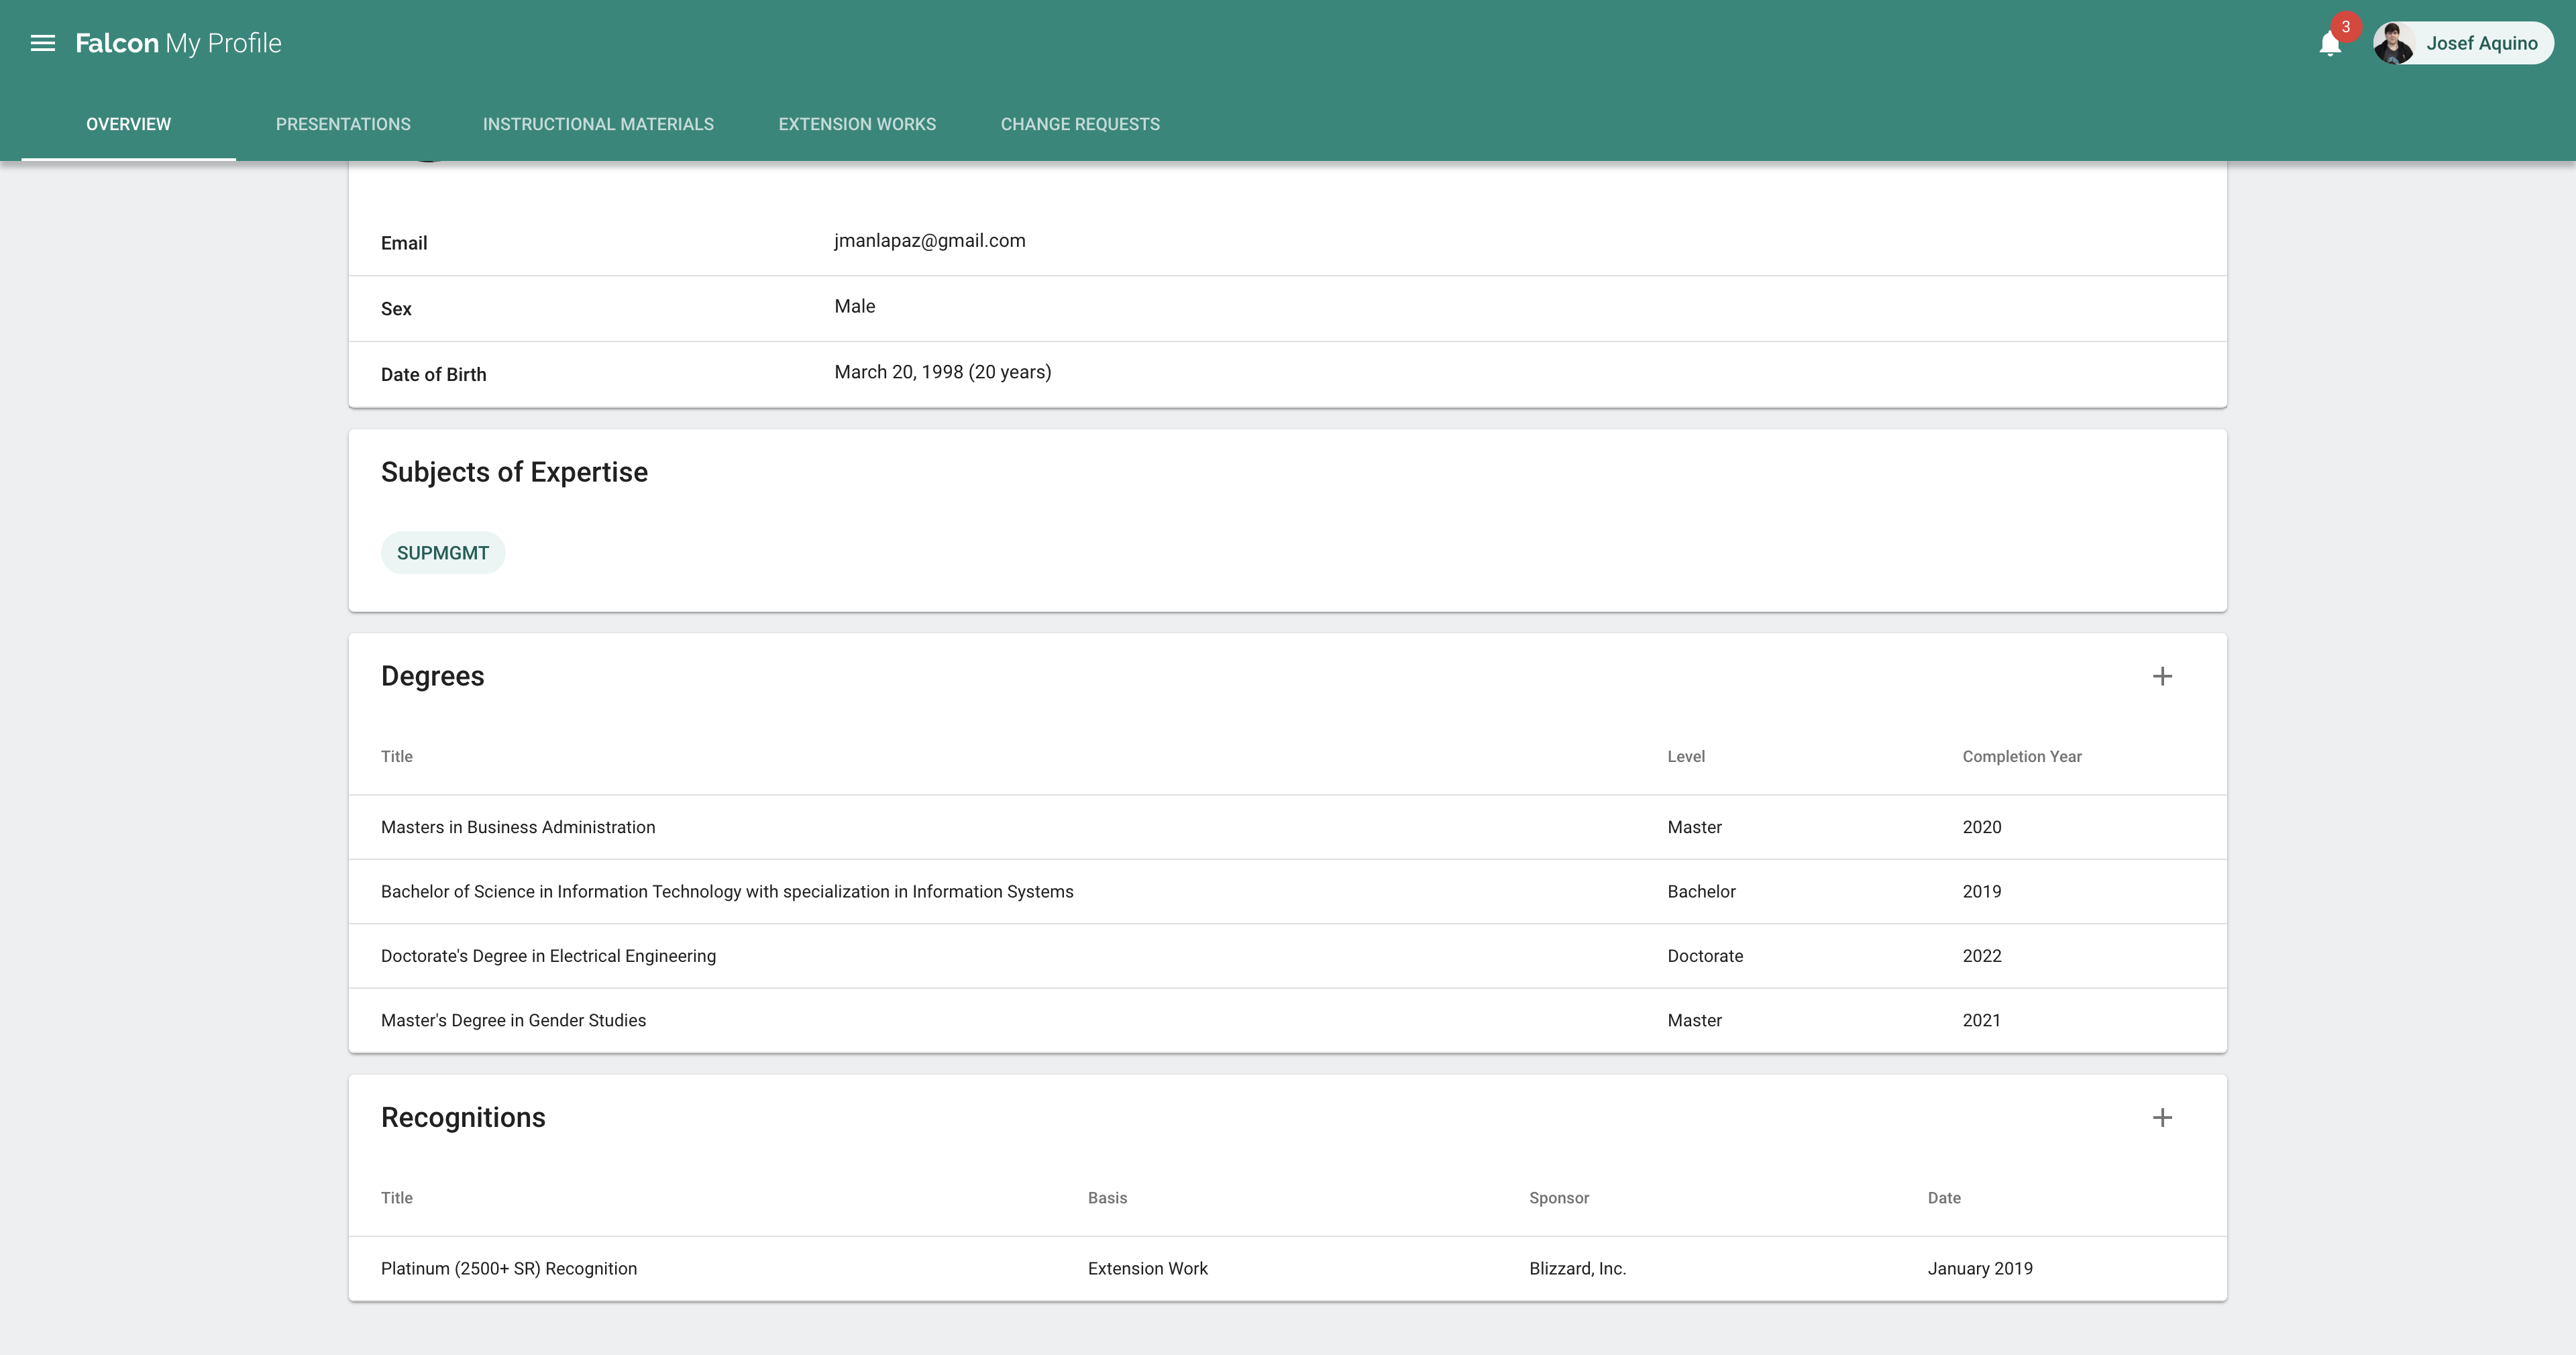
\includegraphics[width=\linewidth]{figures/screen_specifications/myprofile_screens/my_profileB.png}
   \caption{My Profile Overview Screen B}
   }
   
   \pagebreak
   
   \subsubsection{My Profile Presentation}
    
    \field{Screen Name}{My Profile Presentation}
    
    \field{File Name}{$/pages/FacultyProfiles/components/faculty_detail_tabs/PresentationsTab/index.js$}
    
    \field{Description} {Displays the list of presentations}
    
  of the profile. It also shows the details of each presentation, such as the category, date, sponsor, venue, conference, medium, and duration. faculty   \field{Layout}{}
    
\makefigure{!ht}{
   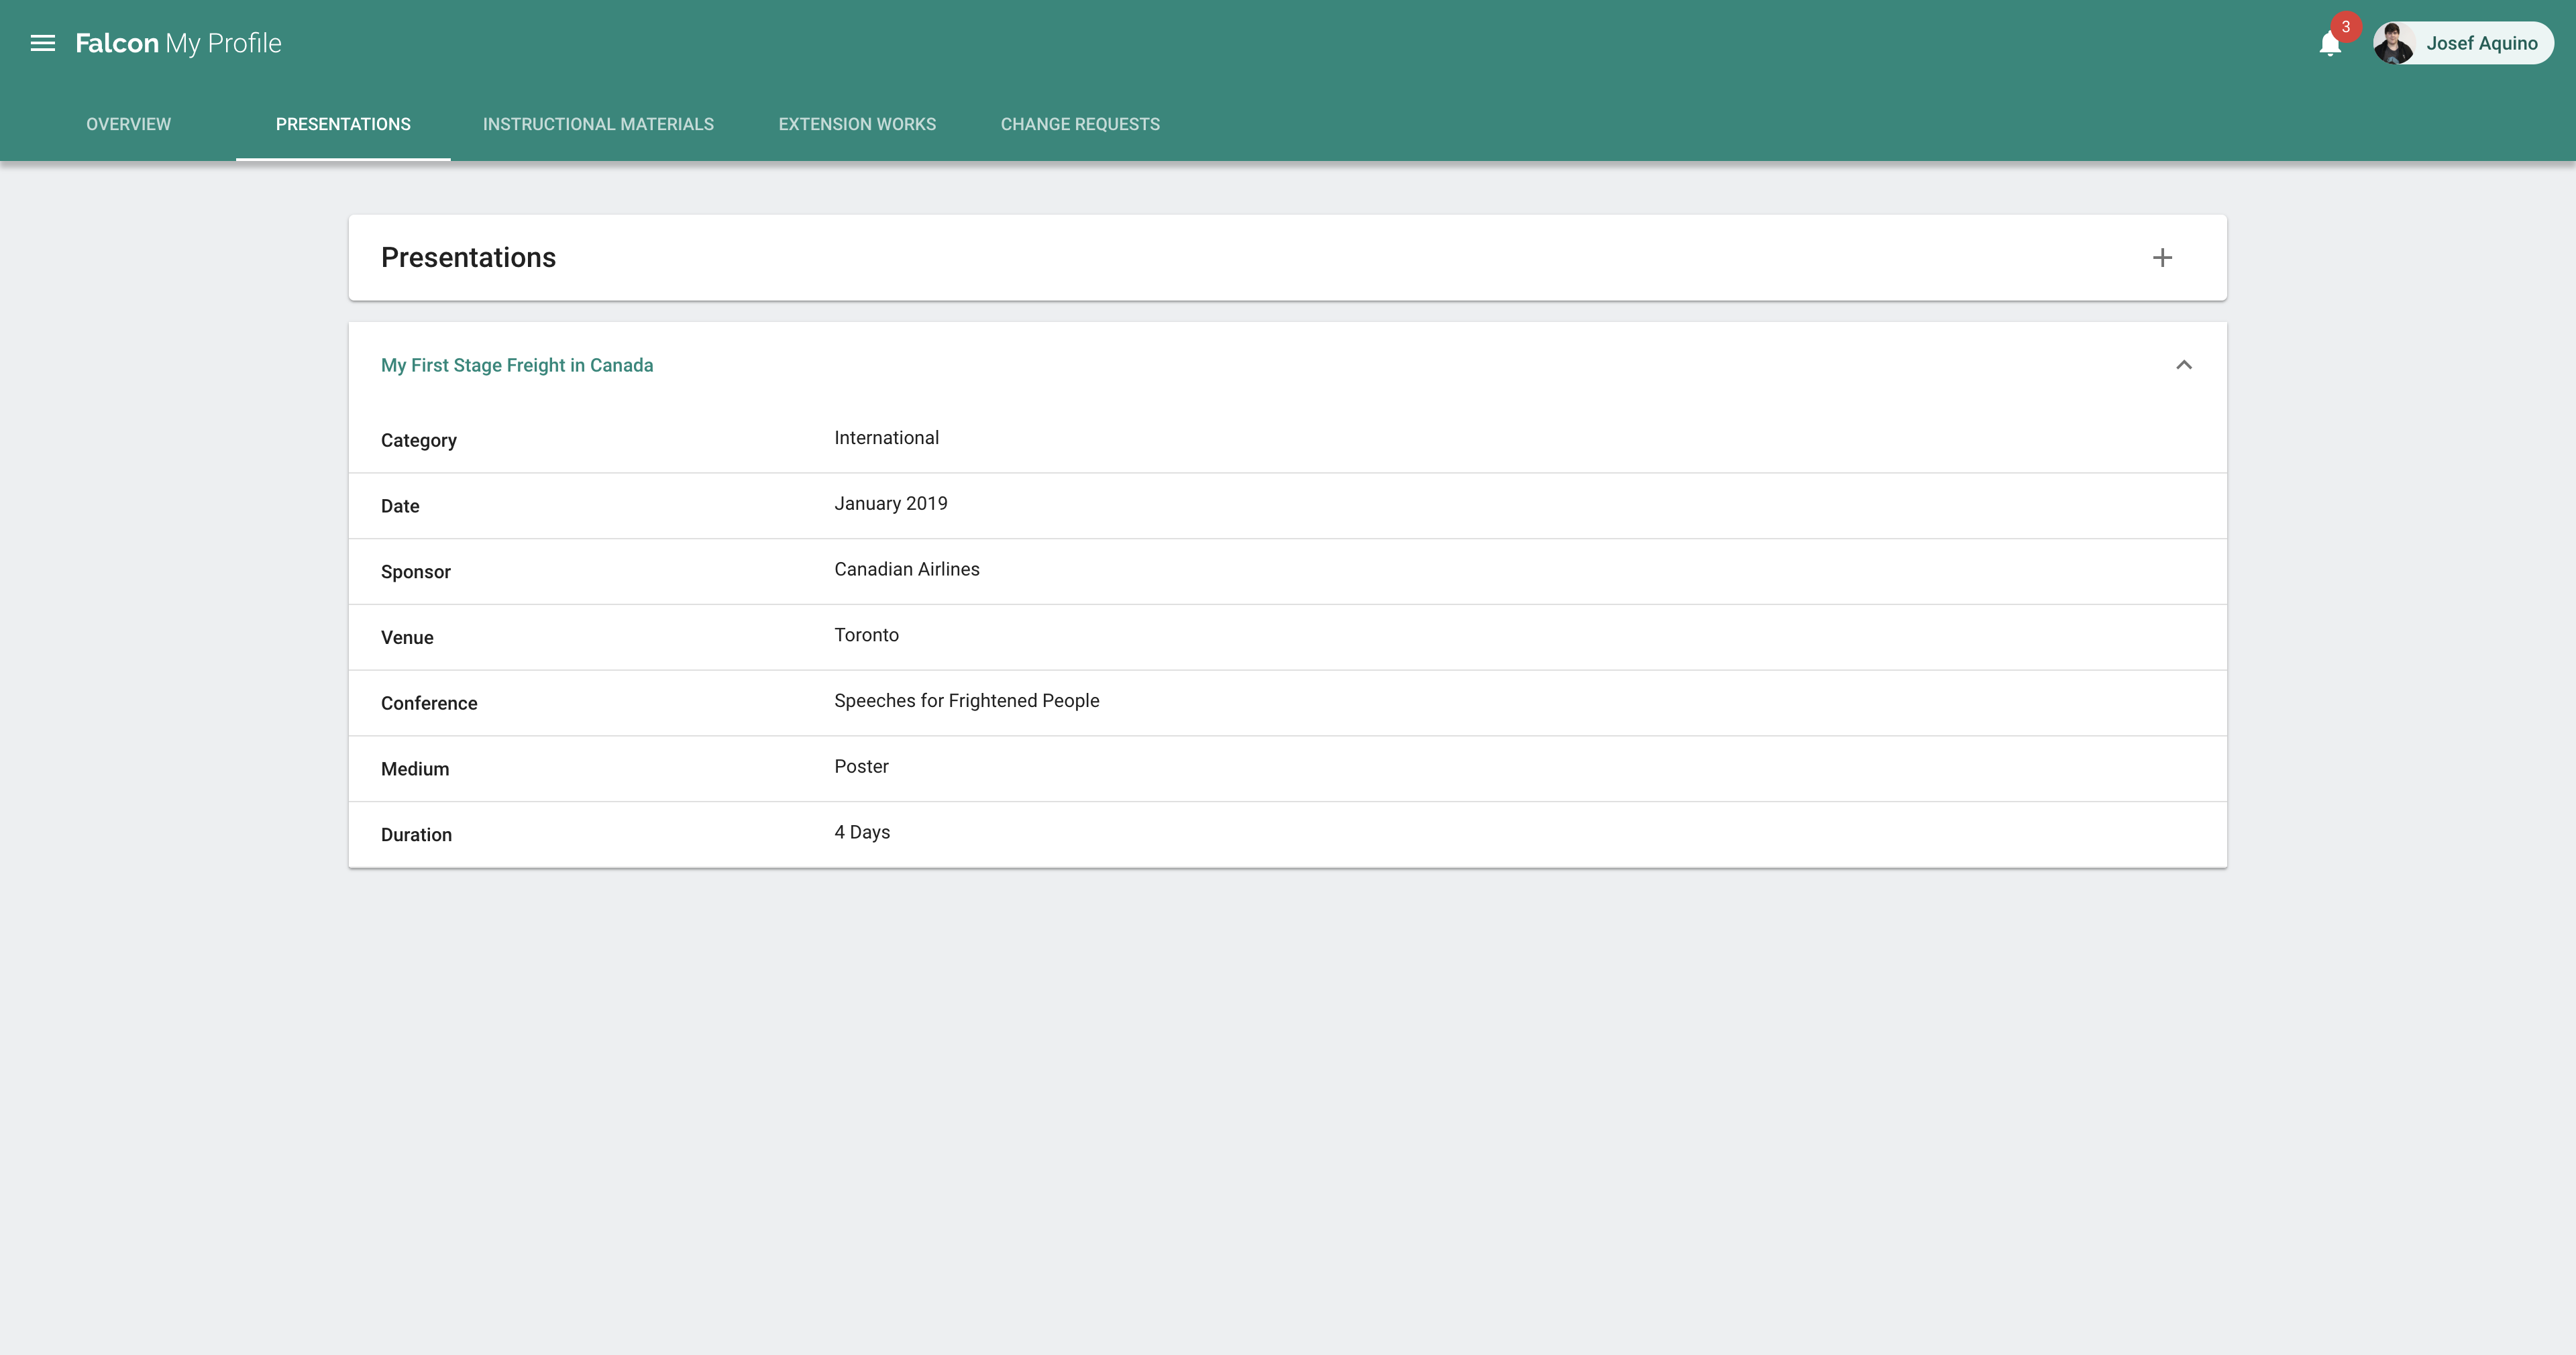
\includegraphics[width=\linewidth]{figures/screen_specifications/myprofile_screens/myprofile_presentation.png}
   \caption{My Profile Presentation Screen A}
   }

    \pagebreak
    
    \subsubsection{My Profile Instructional Materials}
    
    \field{Screen Name}{My Profile Instructional Materials}
    
    \field{File Name}{$/pages/FacultyProfiles/components/faculty_detail_tabs/InstructionalMaterialsTab/index.js$}
    
    \field{Description} {Displays the list of instructional materials of the faculty profile. It also shows the details of each instructional material, such as the category, date, sponsor, venue, conference, medium, and duration.}
    
    \field{Layout}{}
    
\makefigure{!ht}{
   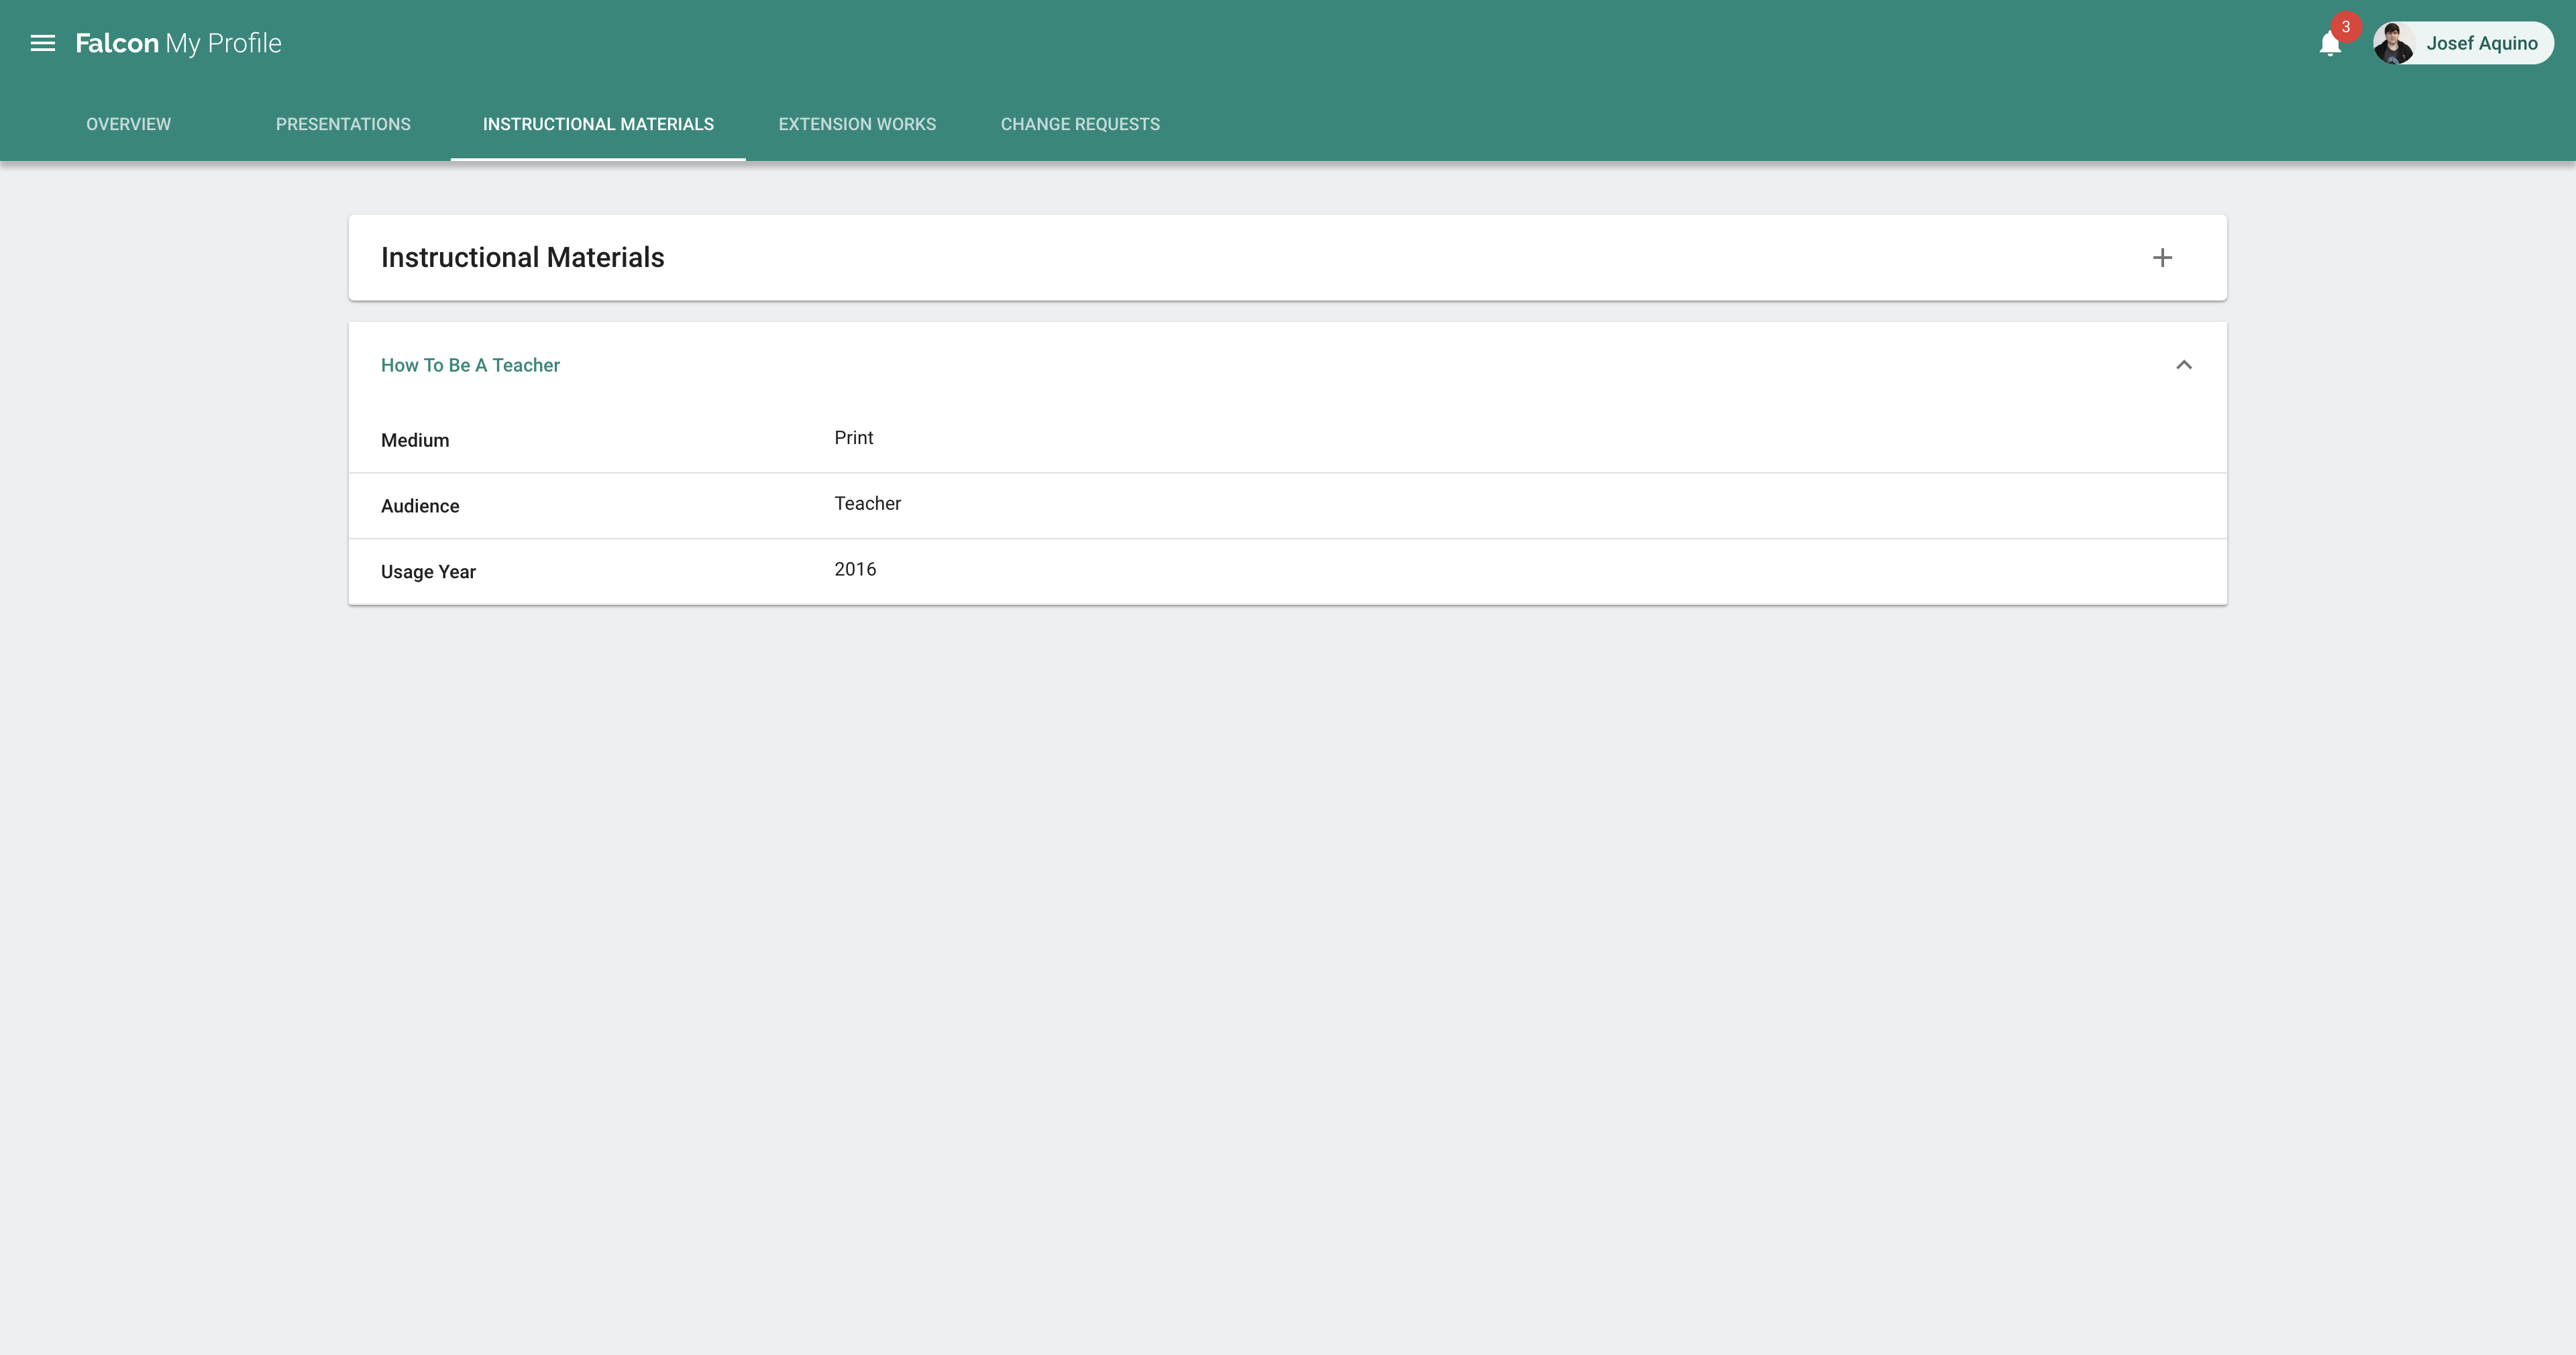
\includegraphics[width=\linewidth]{figures/screen_specifications/myprofile_screens/myprofile_instructional.png}
   \caption{My Profile Presentation Screen}
   }

    \pagebreak
    
    \subsubsection{My Profile Extension Works}
    
    \field{Screen Name}{My Profile Extension Works}
    
    \field{File Name}{$/pages/FacultyProfiles/components/faculty_detail_tabs/ExtensionWorksTab/index.js$}
    
    \field{Description} {Displays the list of extension works of the faculty profile. It also shows the details of each extension work, such as the venue and role.}
    
    \field{Layout}{}
    
\makefigure{!ht}{
   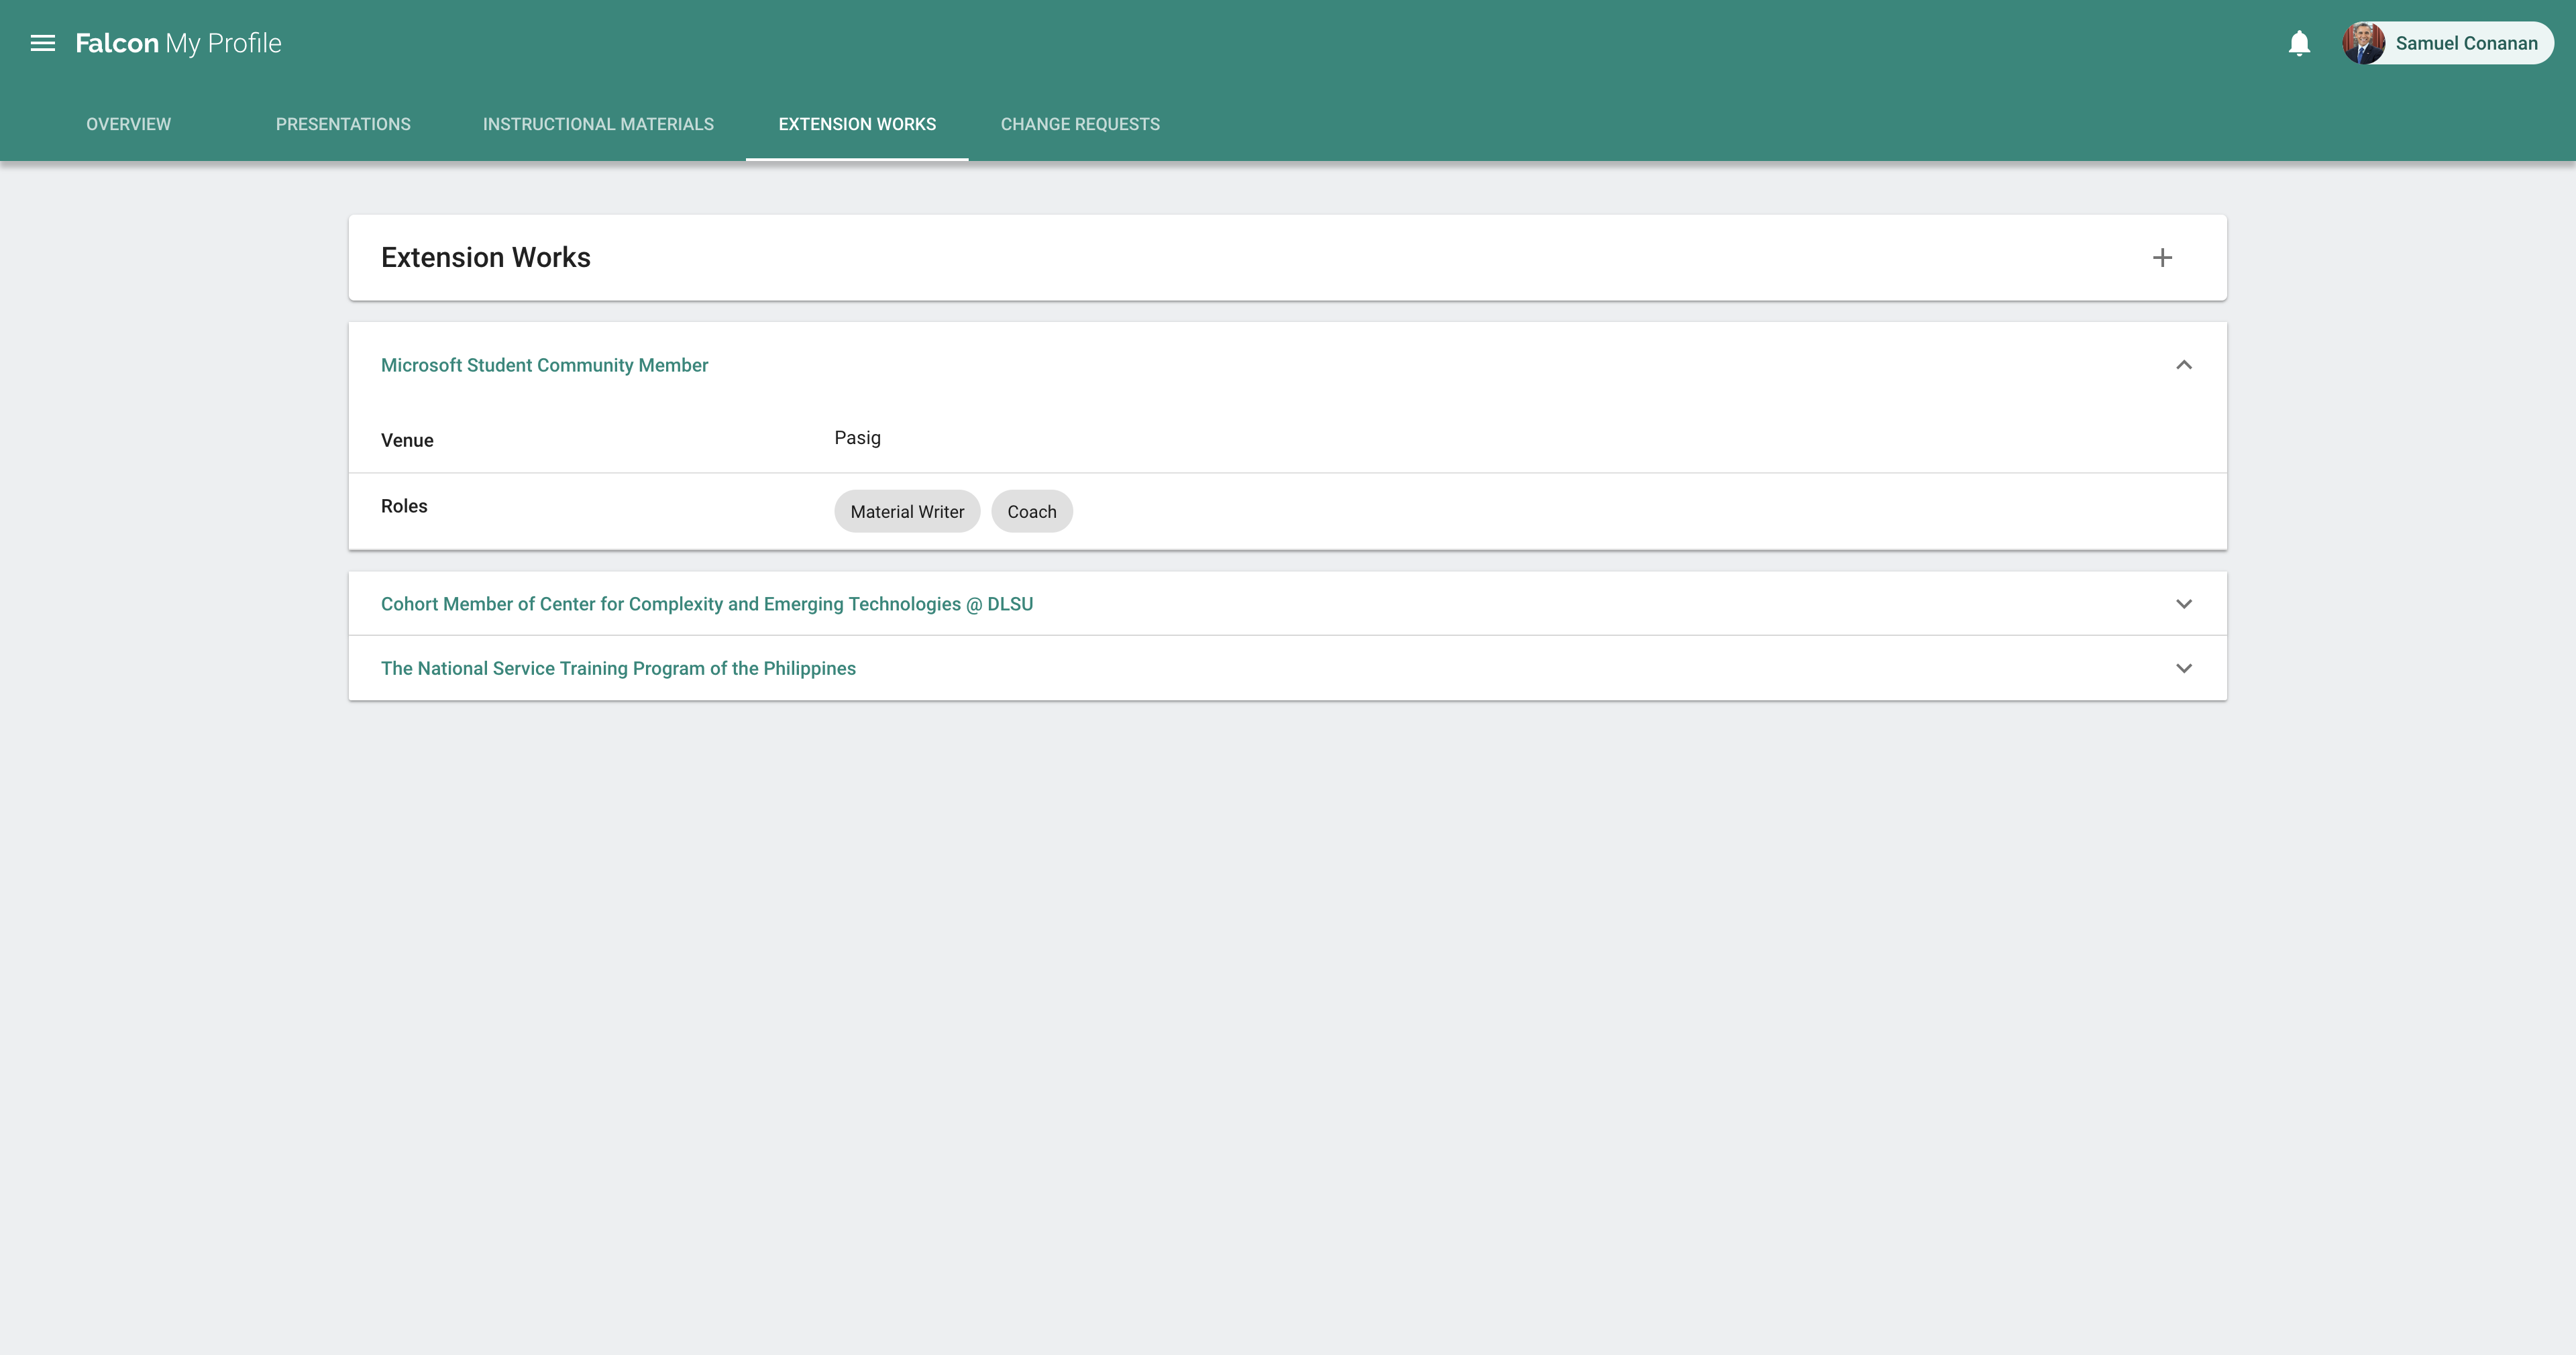
\includegraphics[width=\linewidth]{figures/screen_specifications/myprofile_screens/myprofile_extension.png}
   \caption{My Profile Extension Works Screen}
   }

    \pagebreak
    
    \subsubsection{My Profile Change Requests}
    
    \field{Screen Name}{My Profile Change Requests}
    
    \field{File Name}{$/pages/FacultyProfiles/components/faculty_detail_tabs/ChangeRequestsTab/index.js$}
    
    \field{Description} {Displays the list of change requests of the faculty profile. It also shows the details of each change request and status.}
    
    \field{Layout}{}
    
    \pagebreak
    
\makefigure{!ht}{
   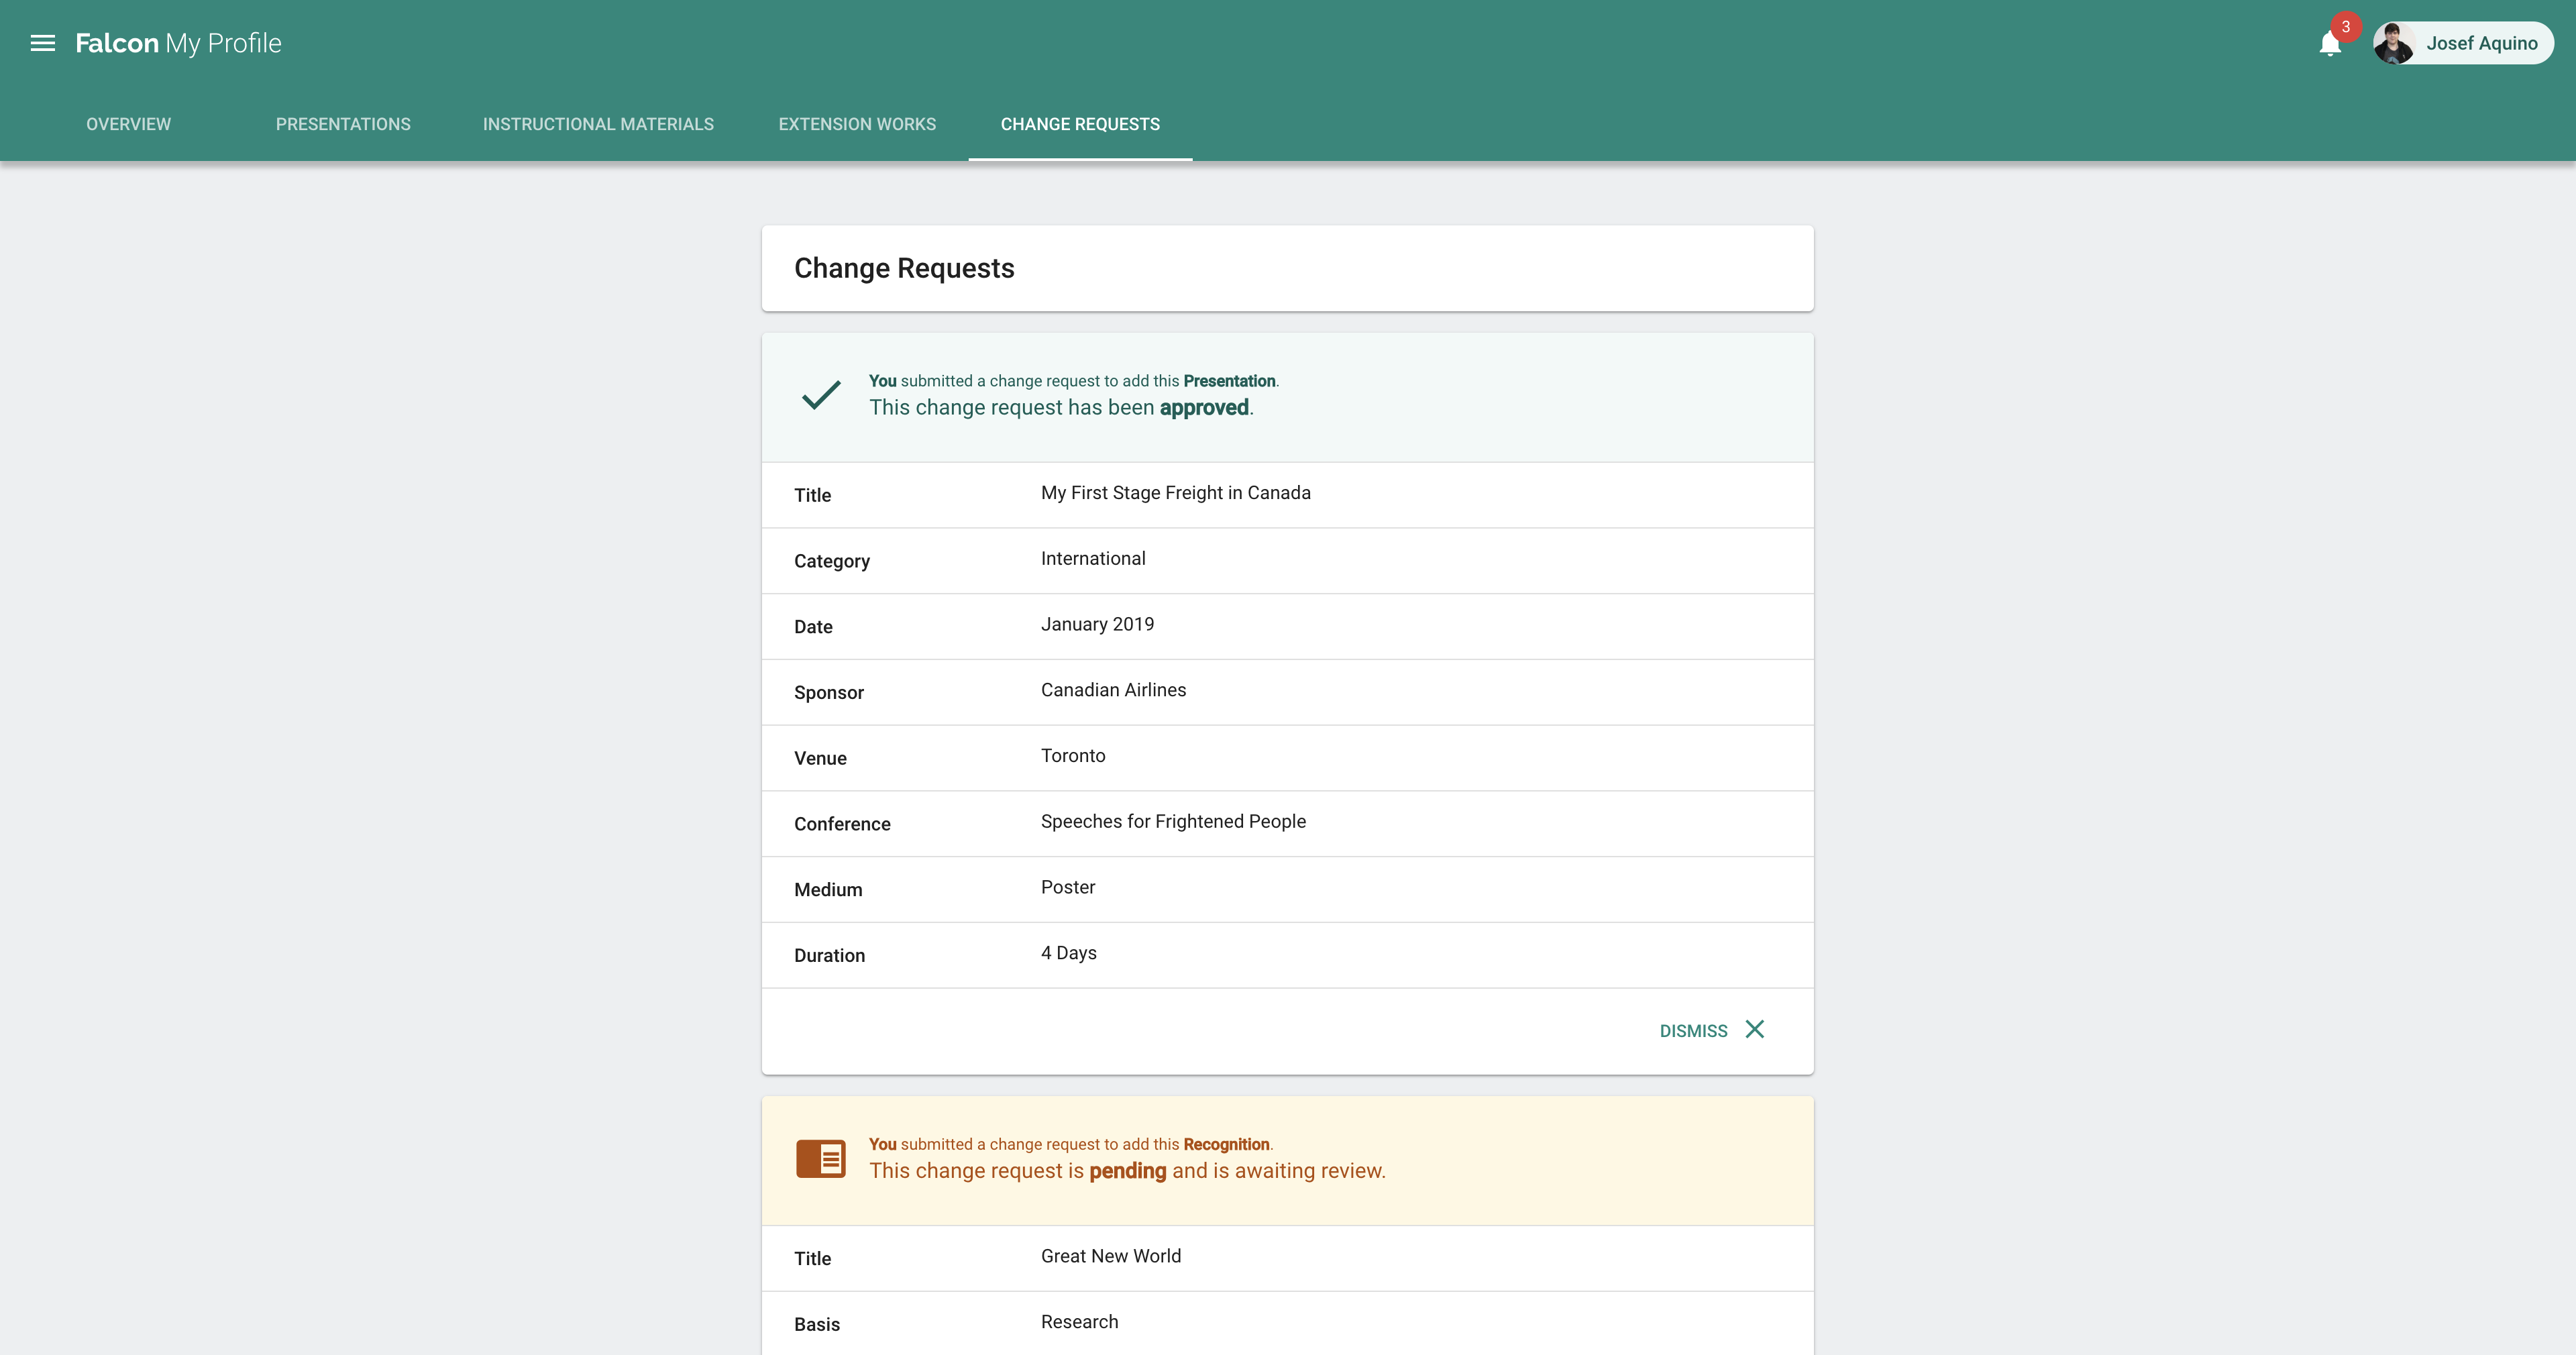
\includegraphics[width=\linewidth]{figures/screen_specifications/myprofile_screens/myprofile_changeA.png}
   \caption{My Profile Change Request A}
   }
   
   
\makefigure{!ht}{
   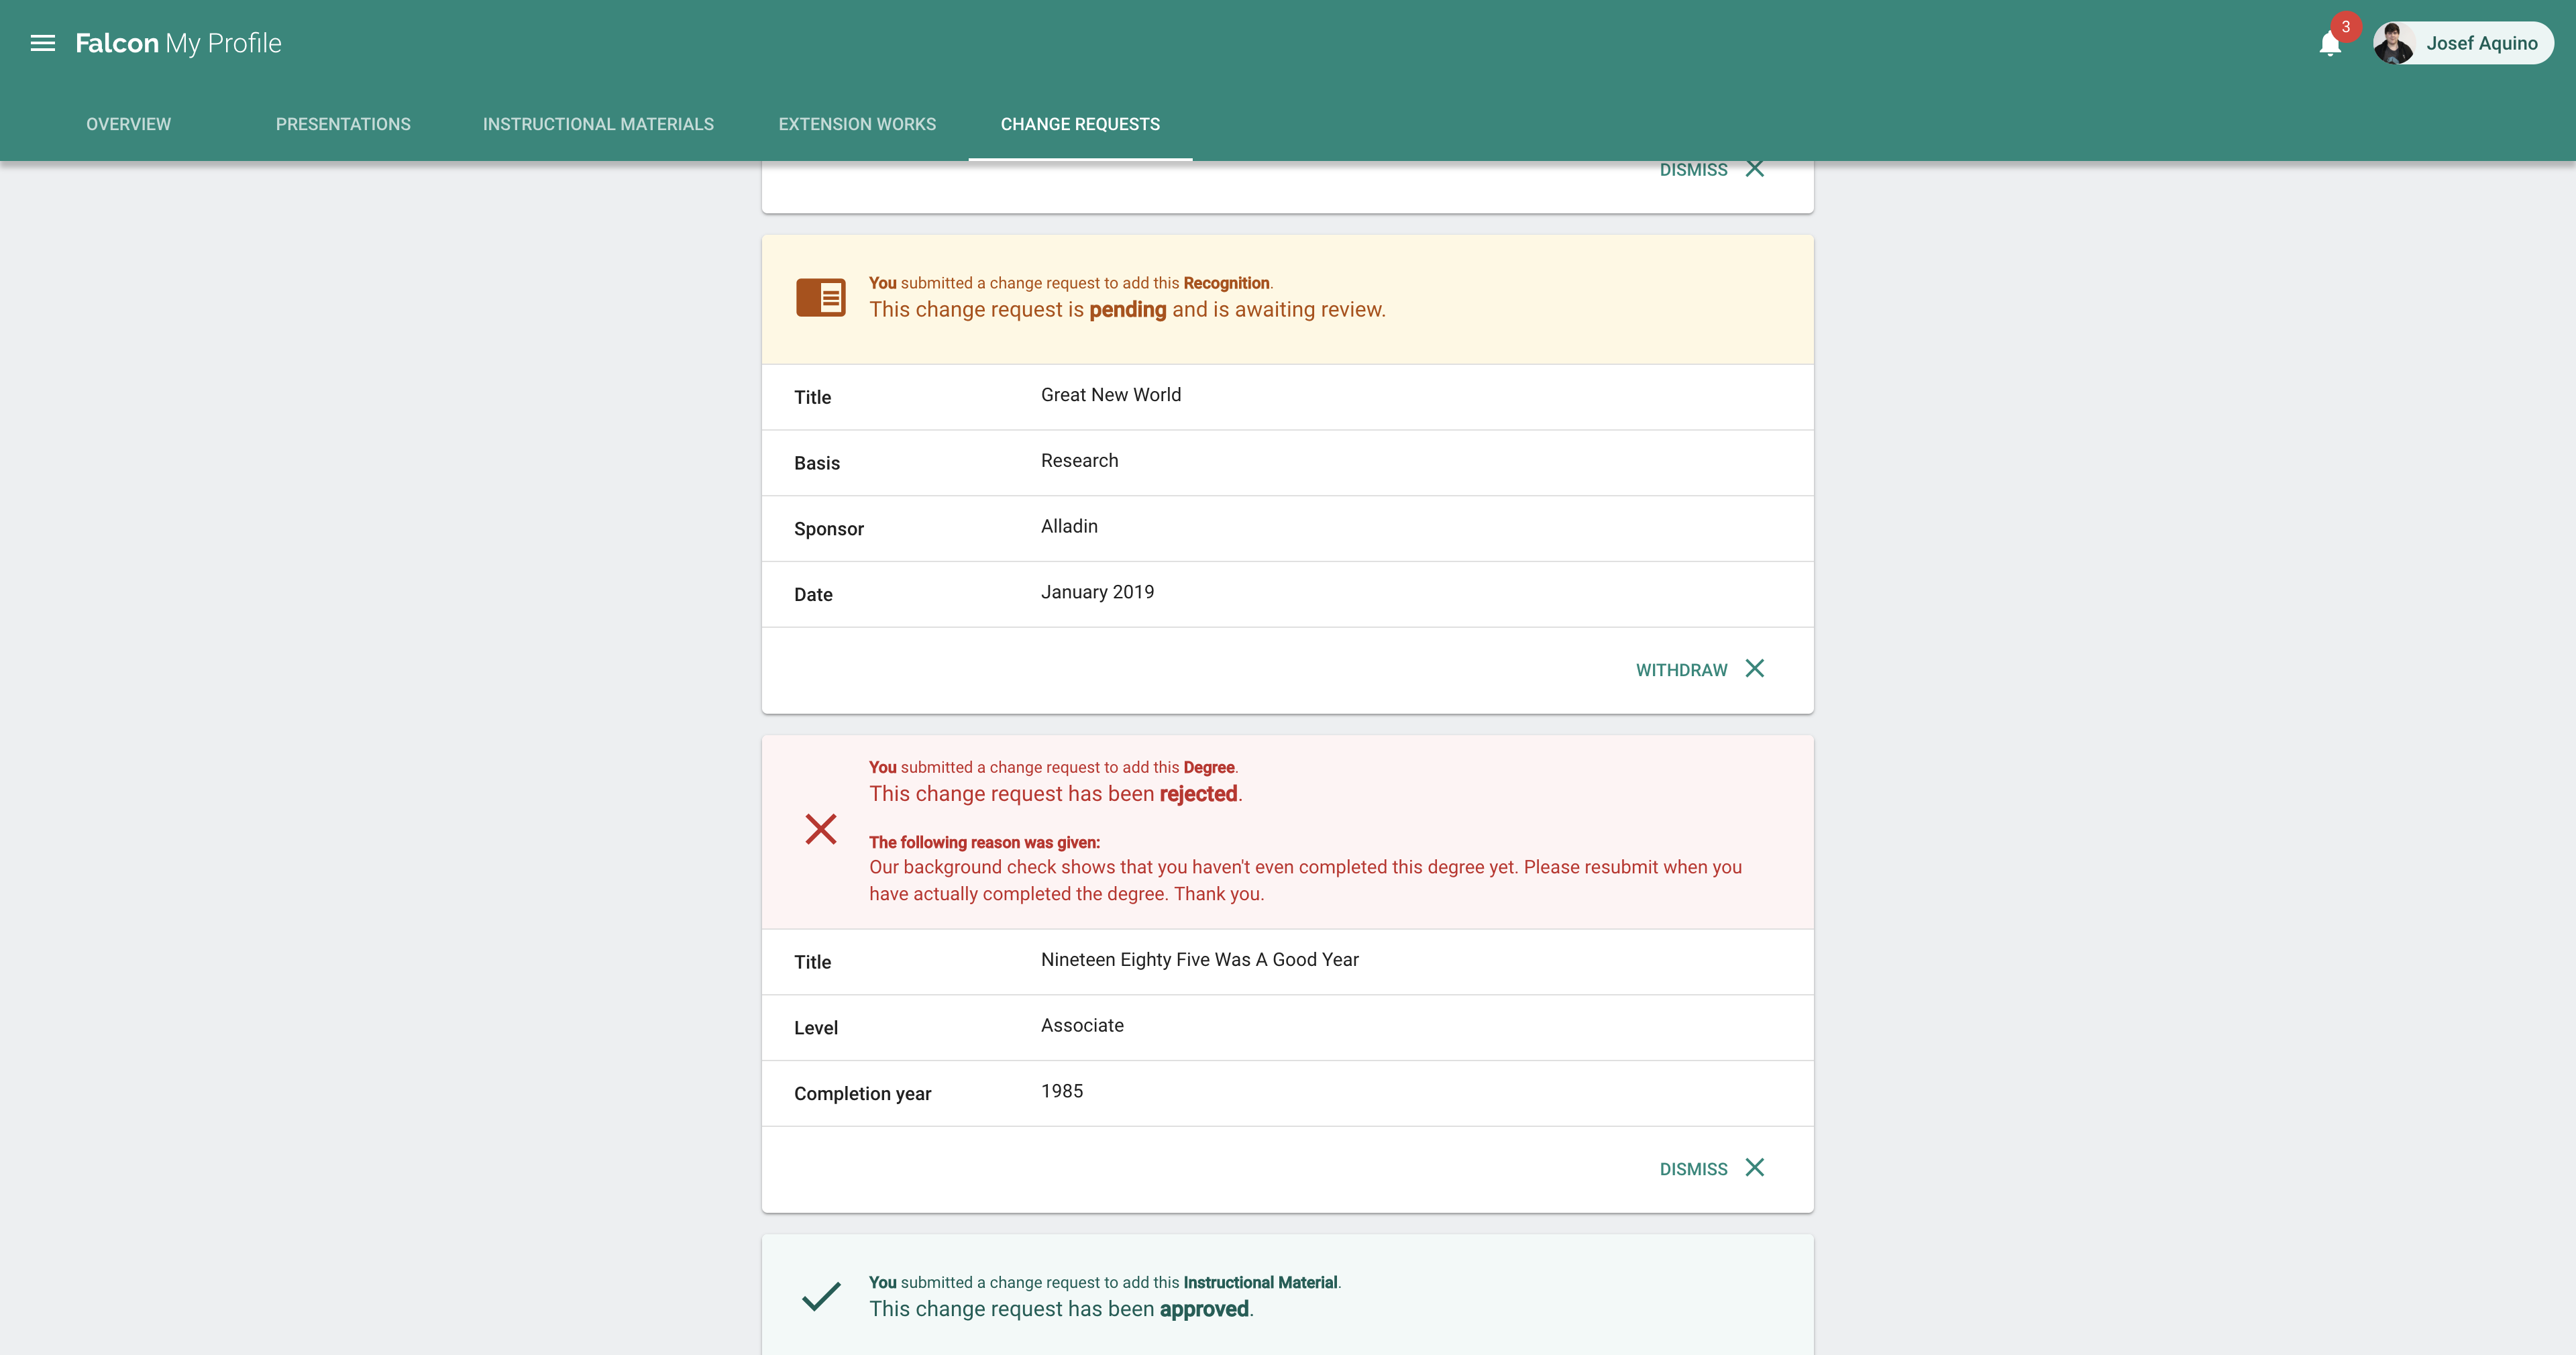
\includegraphics[width=\linewidth]{figures/screen_specifications/myprofile_screens/myprofile_changeB.png}
   \caption{My Profile Change Request B}
   }

    \pagebreak
    
    \subsubsection{My Profile Password Notification}
    
    \field{Screen Name}{My Profile Password Notification}
    
    \field{File Name}{$/pages/SignIn/components/PasswordSetupCard/index.js$}
    
    \field{Description} {Notifies the faculty member that the password for their faculty profile has been reset and they are currently using a temporary password. This also reminds faculty members that they must manually change their password.}
    
    \field{Layout}{}
    
\makefigure{!ht}{
   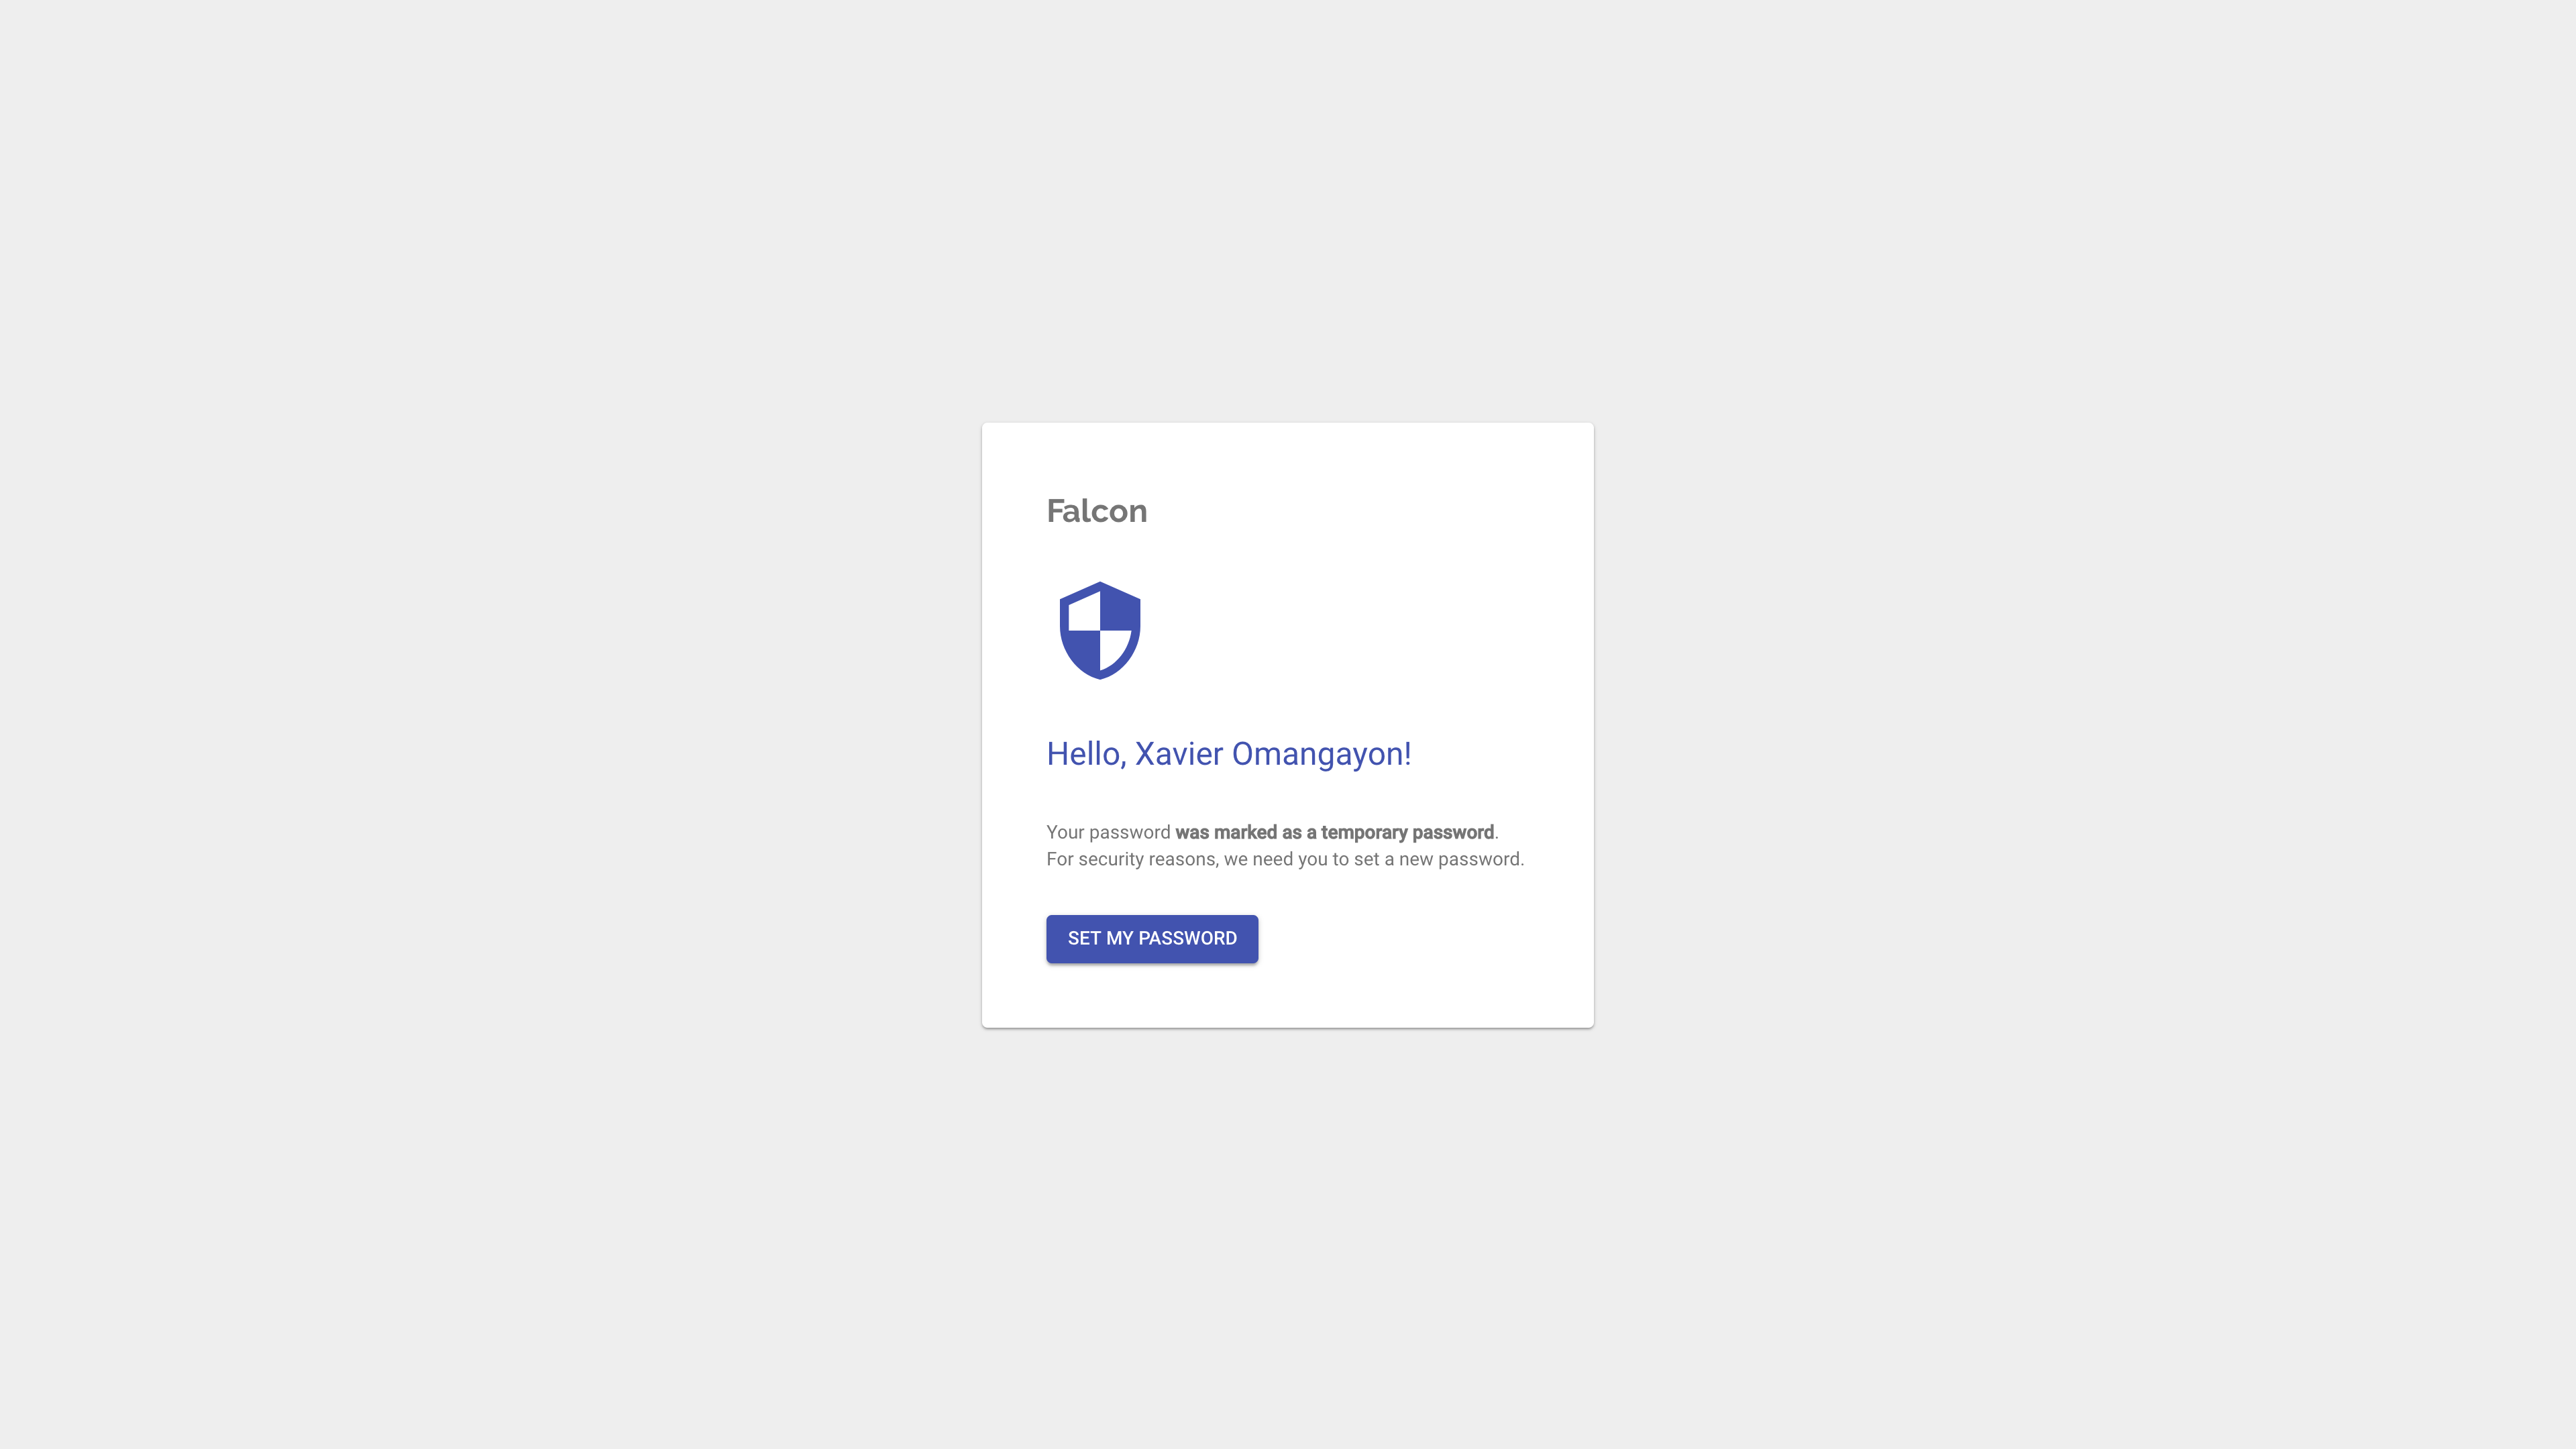
\includegraphics[width=\linewidth]{figures/screen_specifications/myprofile_screens/password_notification.png}
   \caption{My Profile Password Notification Screen}
   }

    \pagebreak
    
    
    \subsection{Faculty Loading}
    
    \subsubsection{Add Classes and Faculties Screen}
    
    \field{Screen Name}{Add Classes and Faculties}
    
    \field{File Name}{$/pages/FacultyLoading/index.js$}
    
    \field{Description} {Displays the schedule where the associate dean adds the classes and faculties.}
    
    \field{Layout}{}
    
\makefigure{!ht}{
   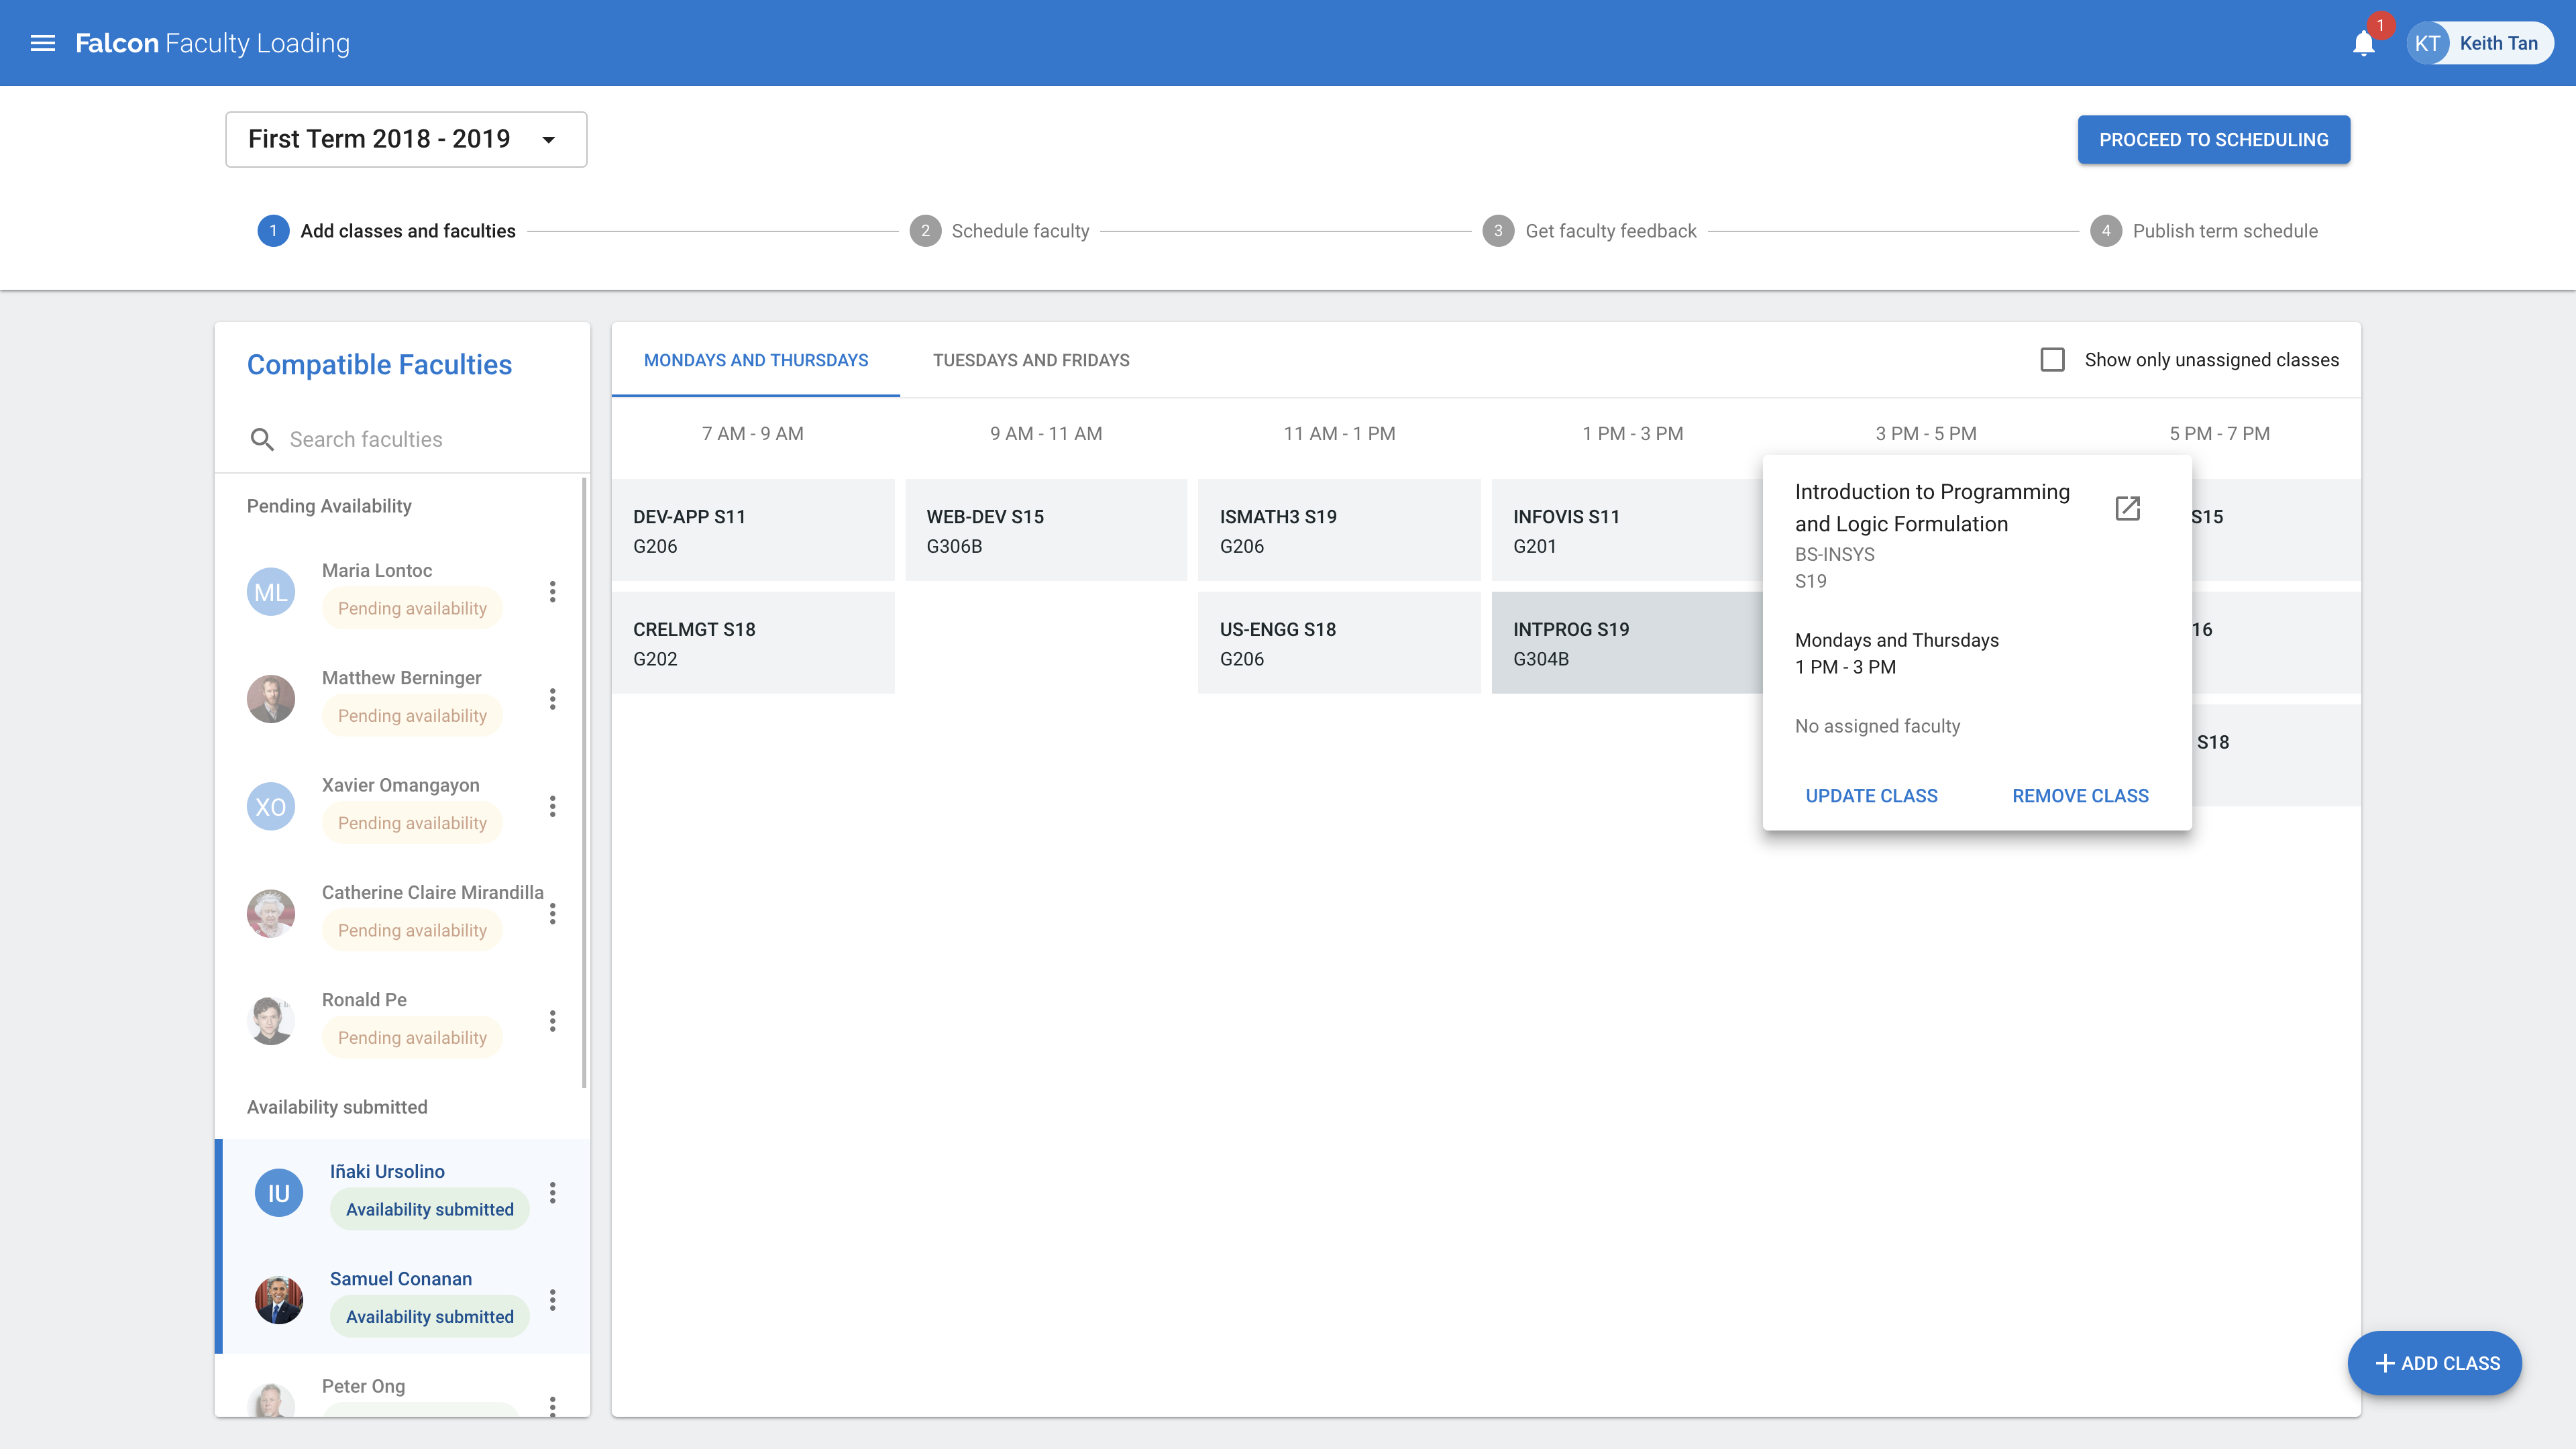
\includegraphics[width=\linewidth]{figures/screen_specifications/faculty_loading_screens/add_classes_screen.png}
   \caption{Add Classes and Faculties Screen}
   }
   
   \pagebreak
   
    \subsubsection{Schedule Faculty Screen}
    
    \field{Screen Name}{Schedule Faculty}
    
    \field{File Name}{$/pages/FacultyLoading/index.js$}
    
    \field{Description} {Displays the schedule where the associate dean can now assign faculty to their classes.}
    
    \field{Layout}{}
    
\makefigure{!ht}{
   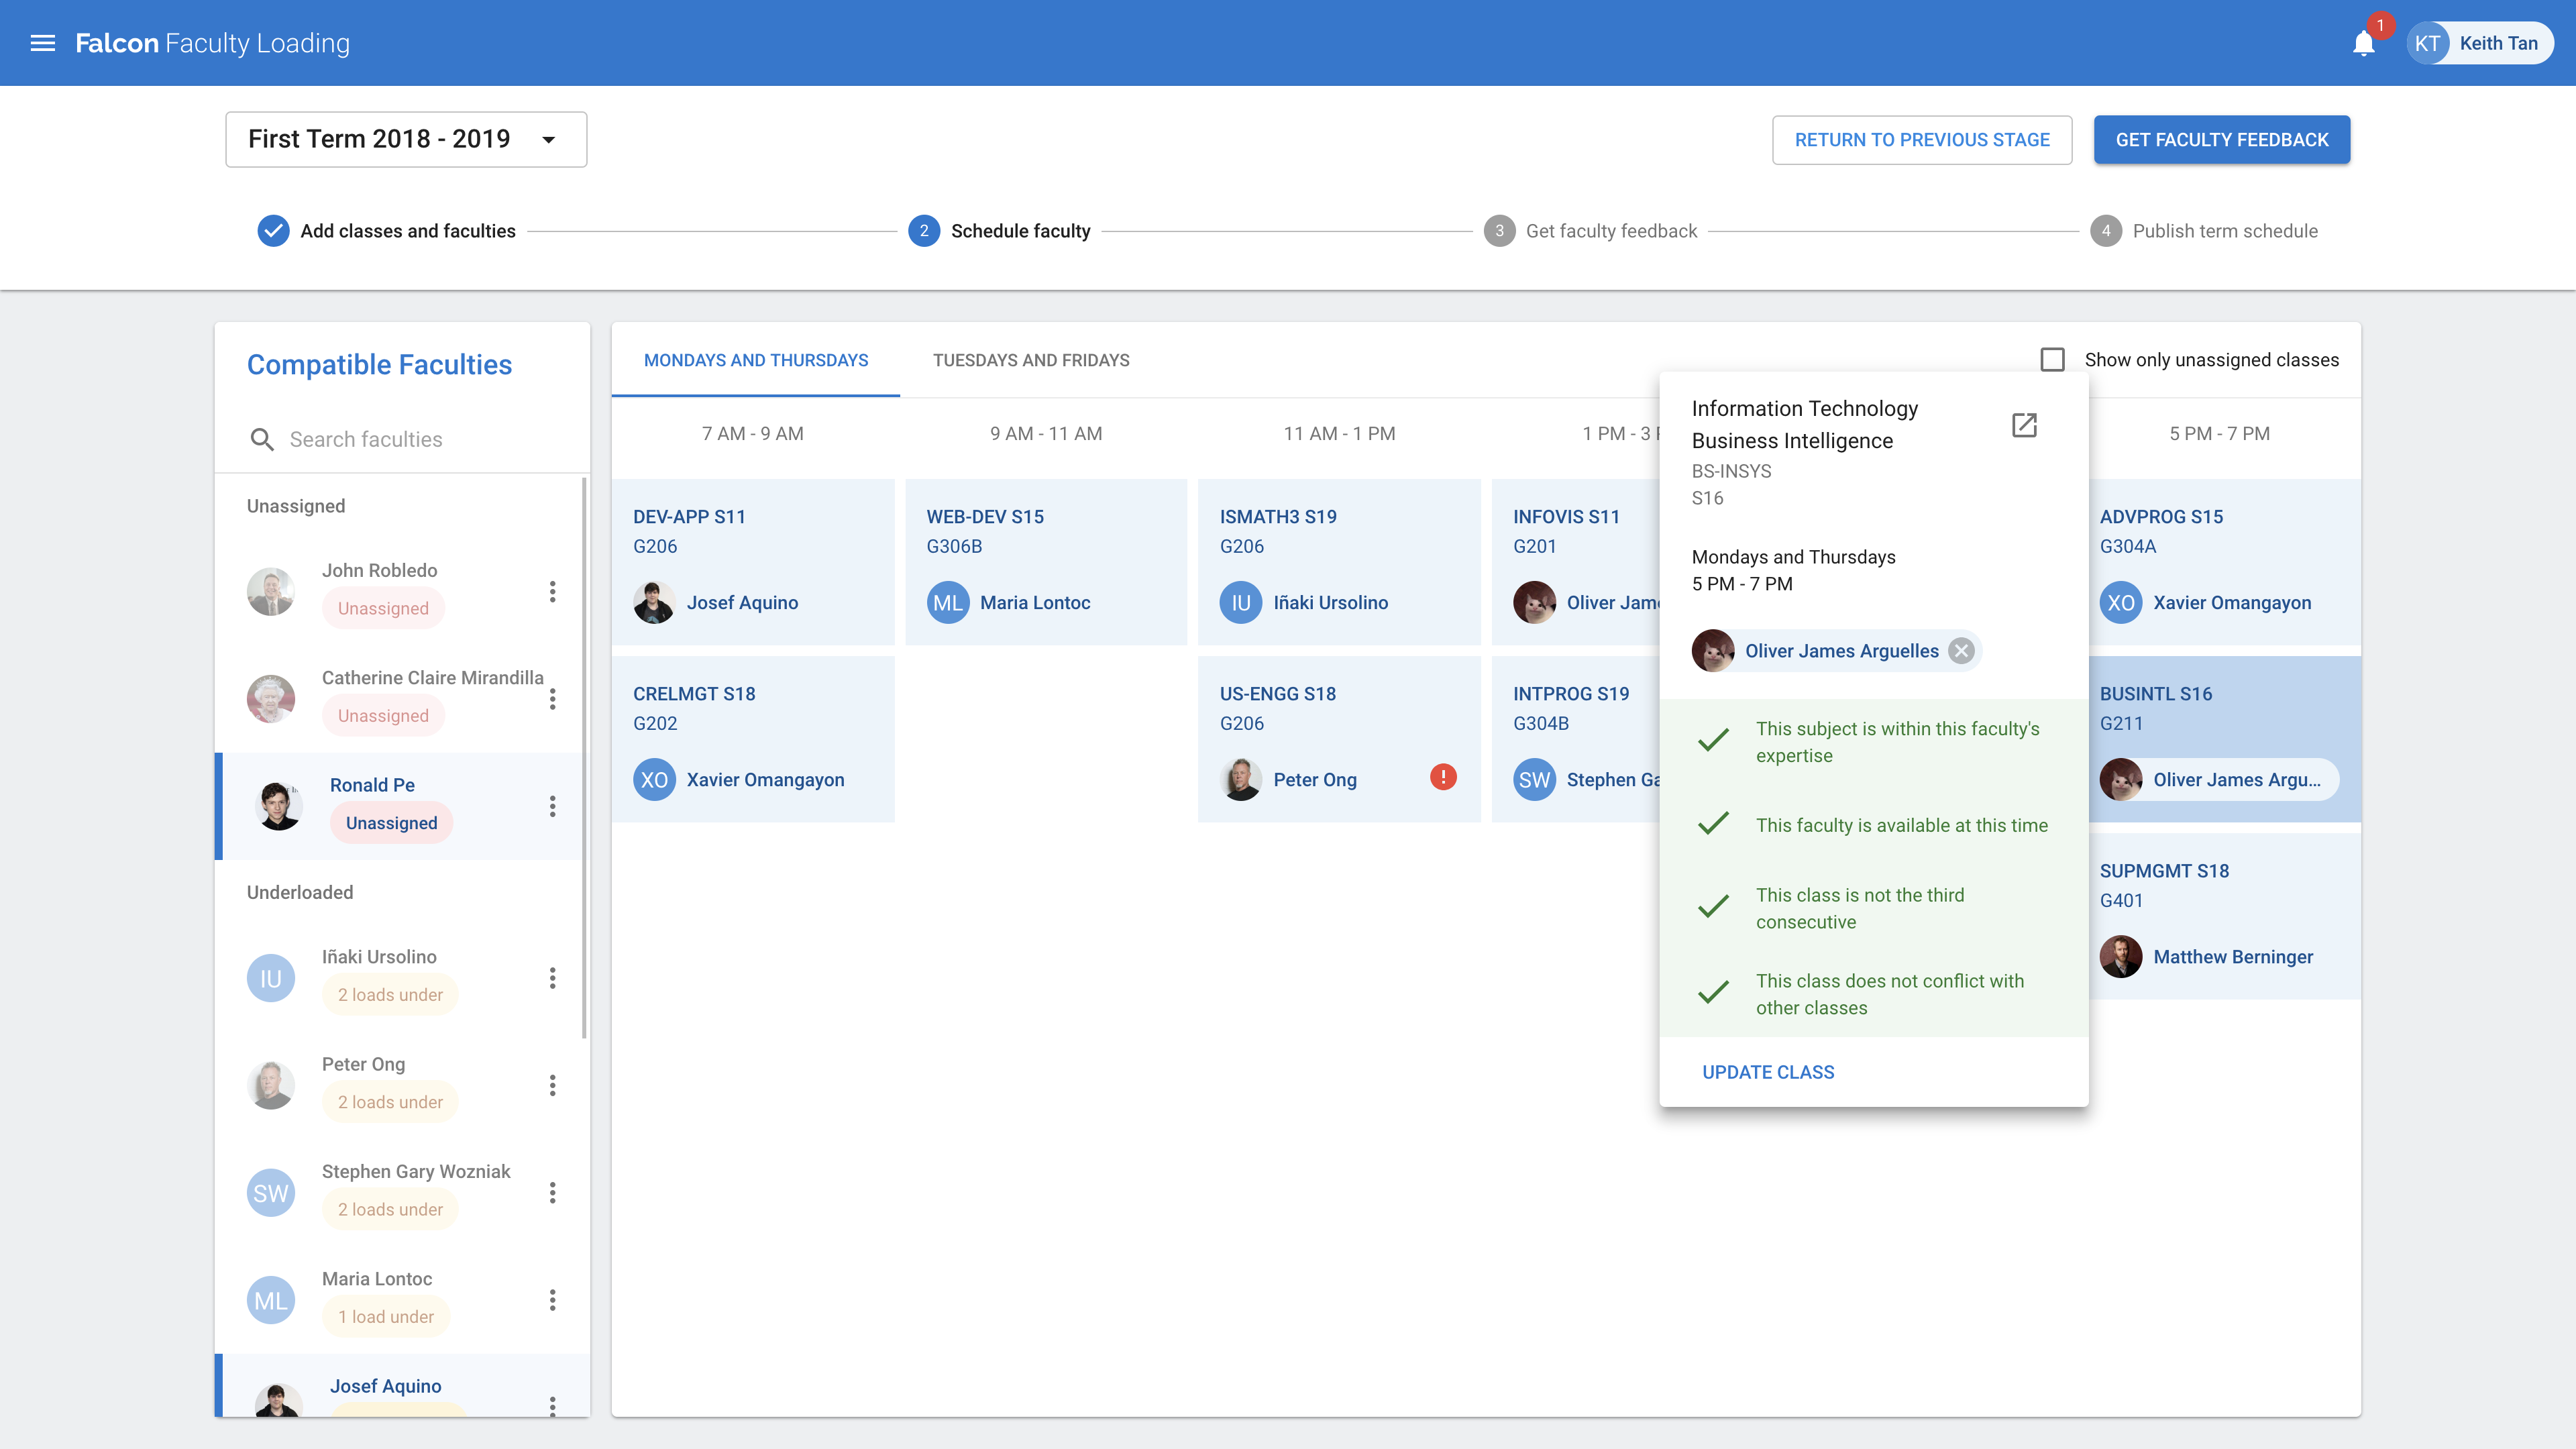
\includegraphics[width=\linewidth]{figures/screen_specifications/faculty_loading_screens/schedule_faculty.png}
   \caption{Schedule Faculty Screen}
   }
   
   \pagebreak
   
   
   \subsubsection{Get Faculty Feedback Screen}
    
    \field{Screen Name}{Get Faculty Feedback}
    
    \field{File Name}{$/pages/FacultyLoading/index.js$}
    
    \field{Description} {Displays the schedule and the associate dean may start receiving feedback from the faculty on their acceptance or rejection of the schedule.}
    
    \field{Layout}{}
    
\makefigure{!ht}{
   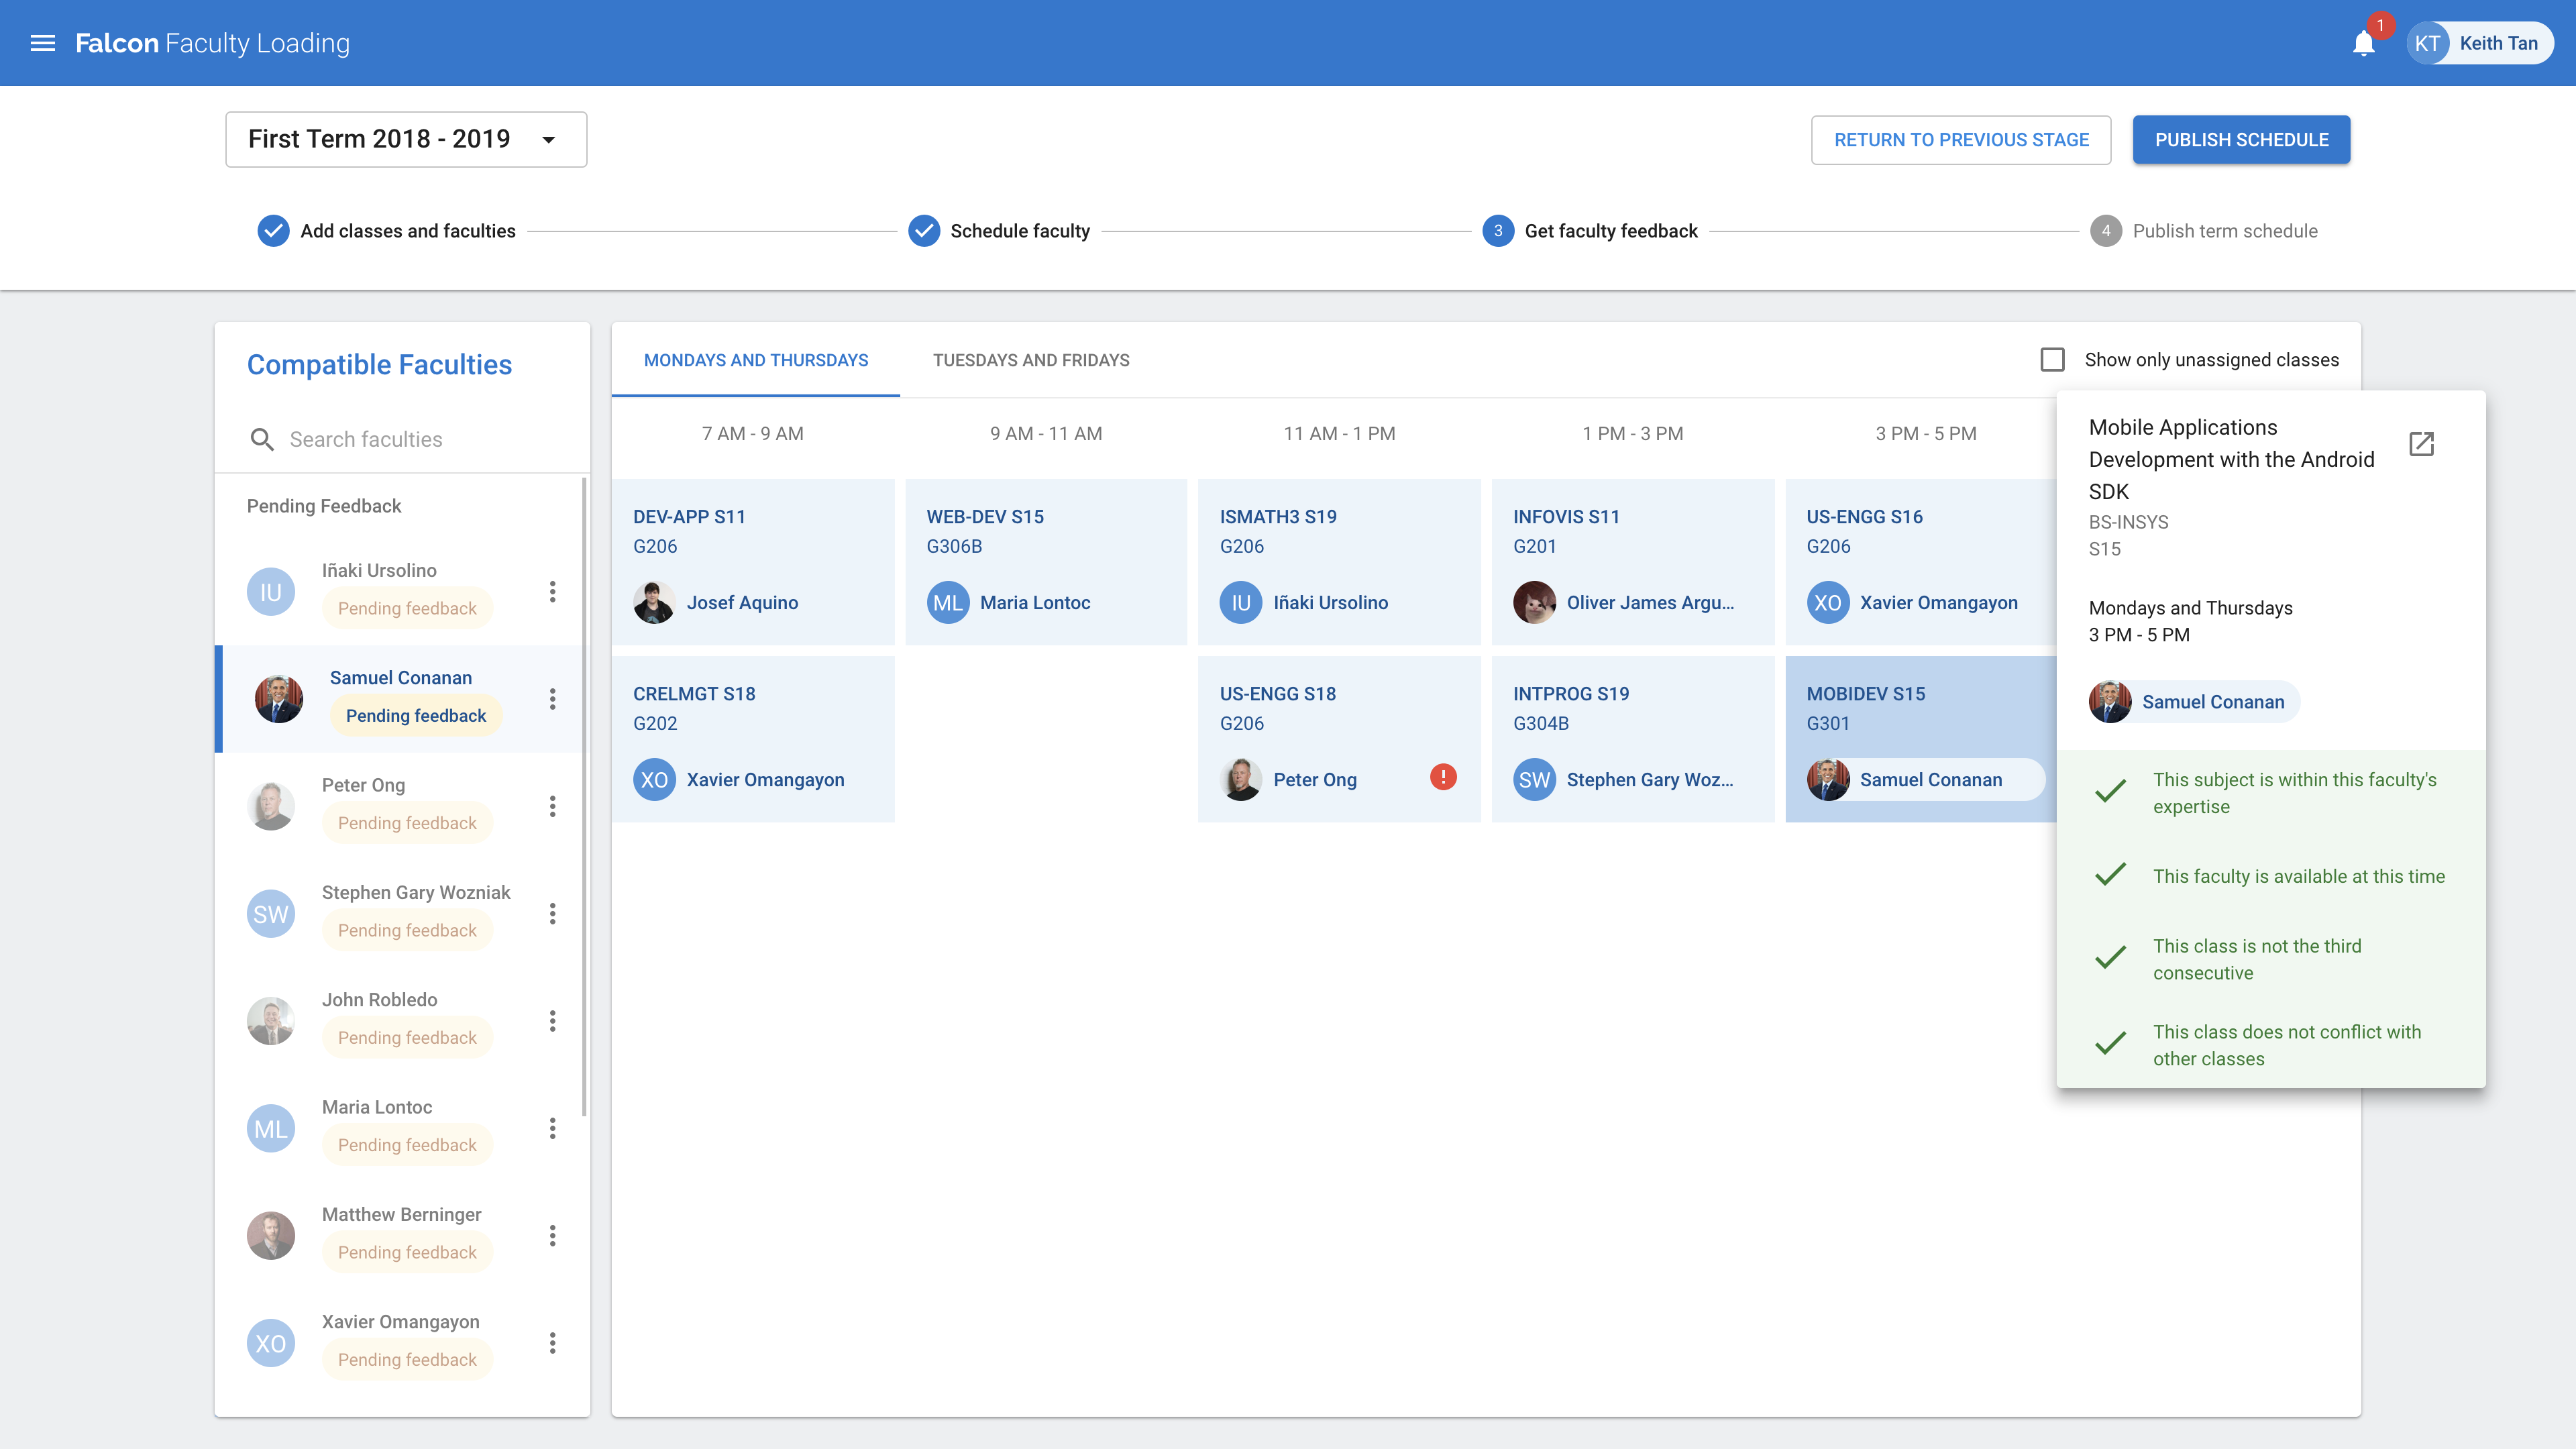
\includegraphics[width=\linewidth]{figures/screen_specifications/faculty_loading_screens/get_feedback.png}
   \caption{Get Faculty Feedback Screen}
   }
   
   \pagebreak
   
    \subsubsection{Publish Schedule Screen}
    
    \field{Screen Name}{Publish Schedule}
    
    \field{File Name}{$/pages/FacultyLoading/index.js$}
    
    \field{Description} {Displays the schedule of the term after it has already been published.}
    
    \field{Layout}{}
    
\makefigure{!ht}{
   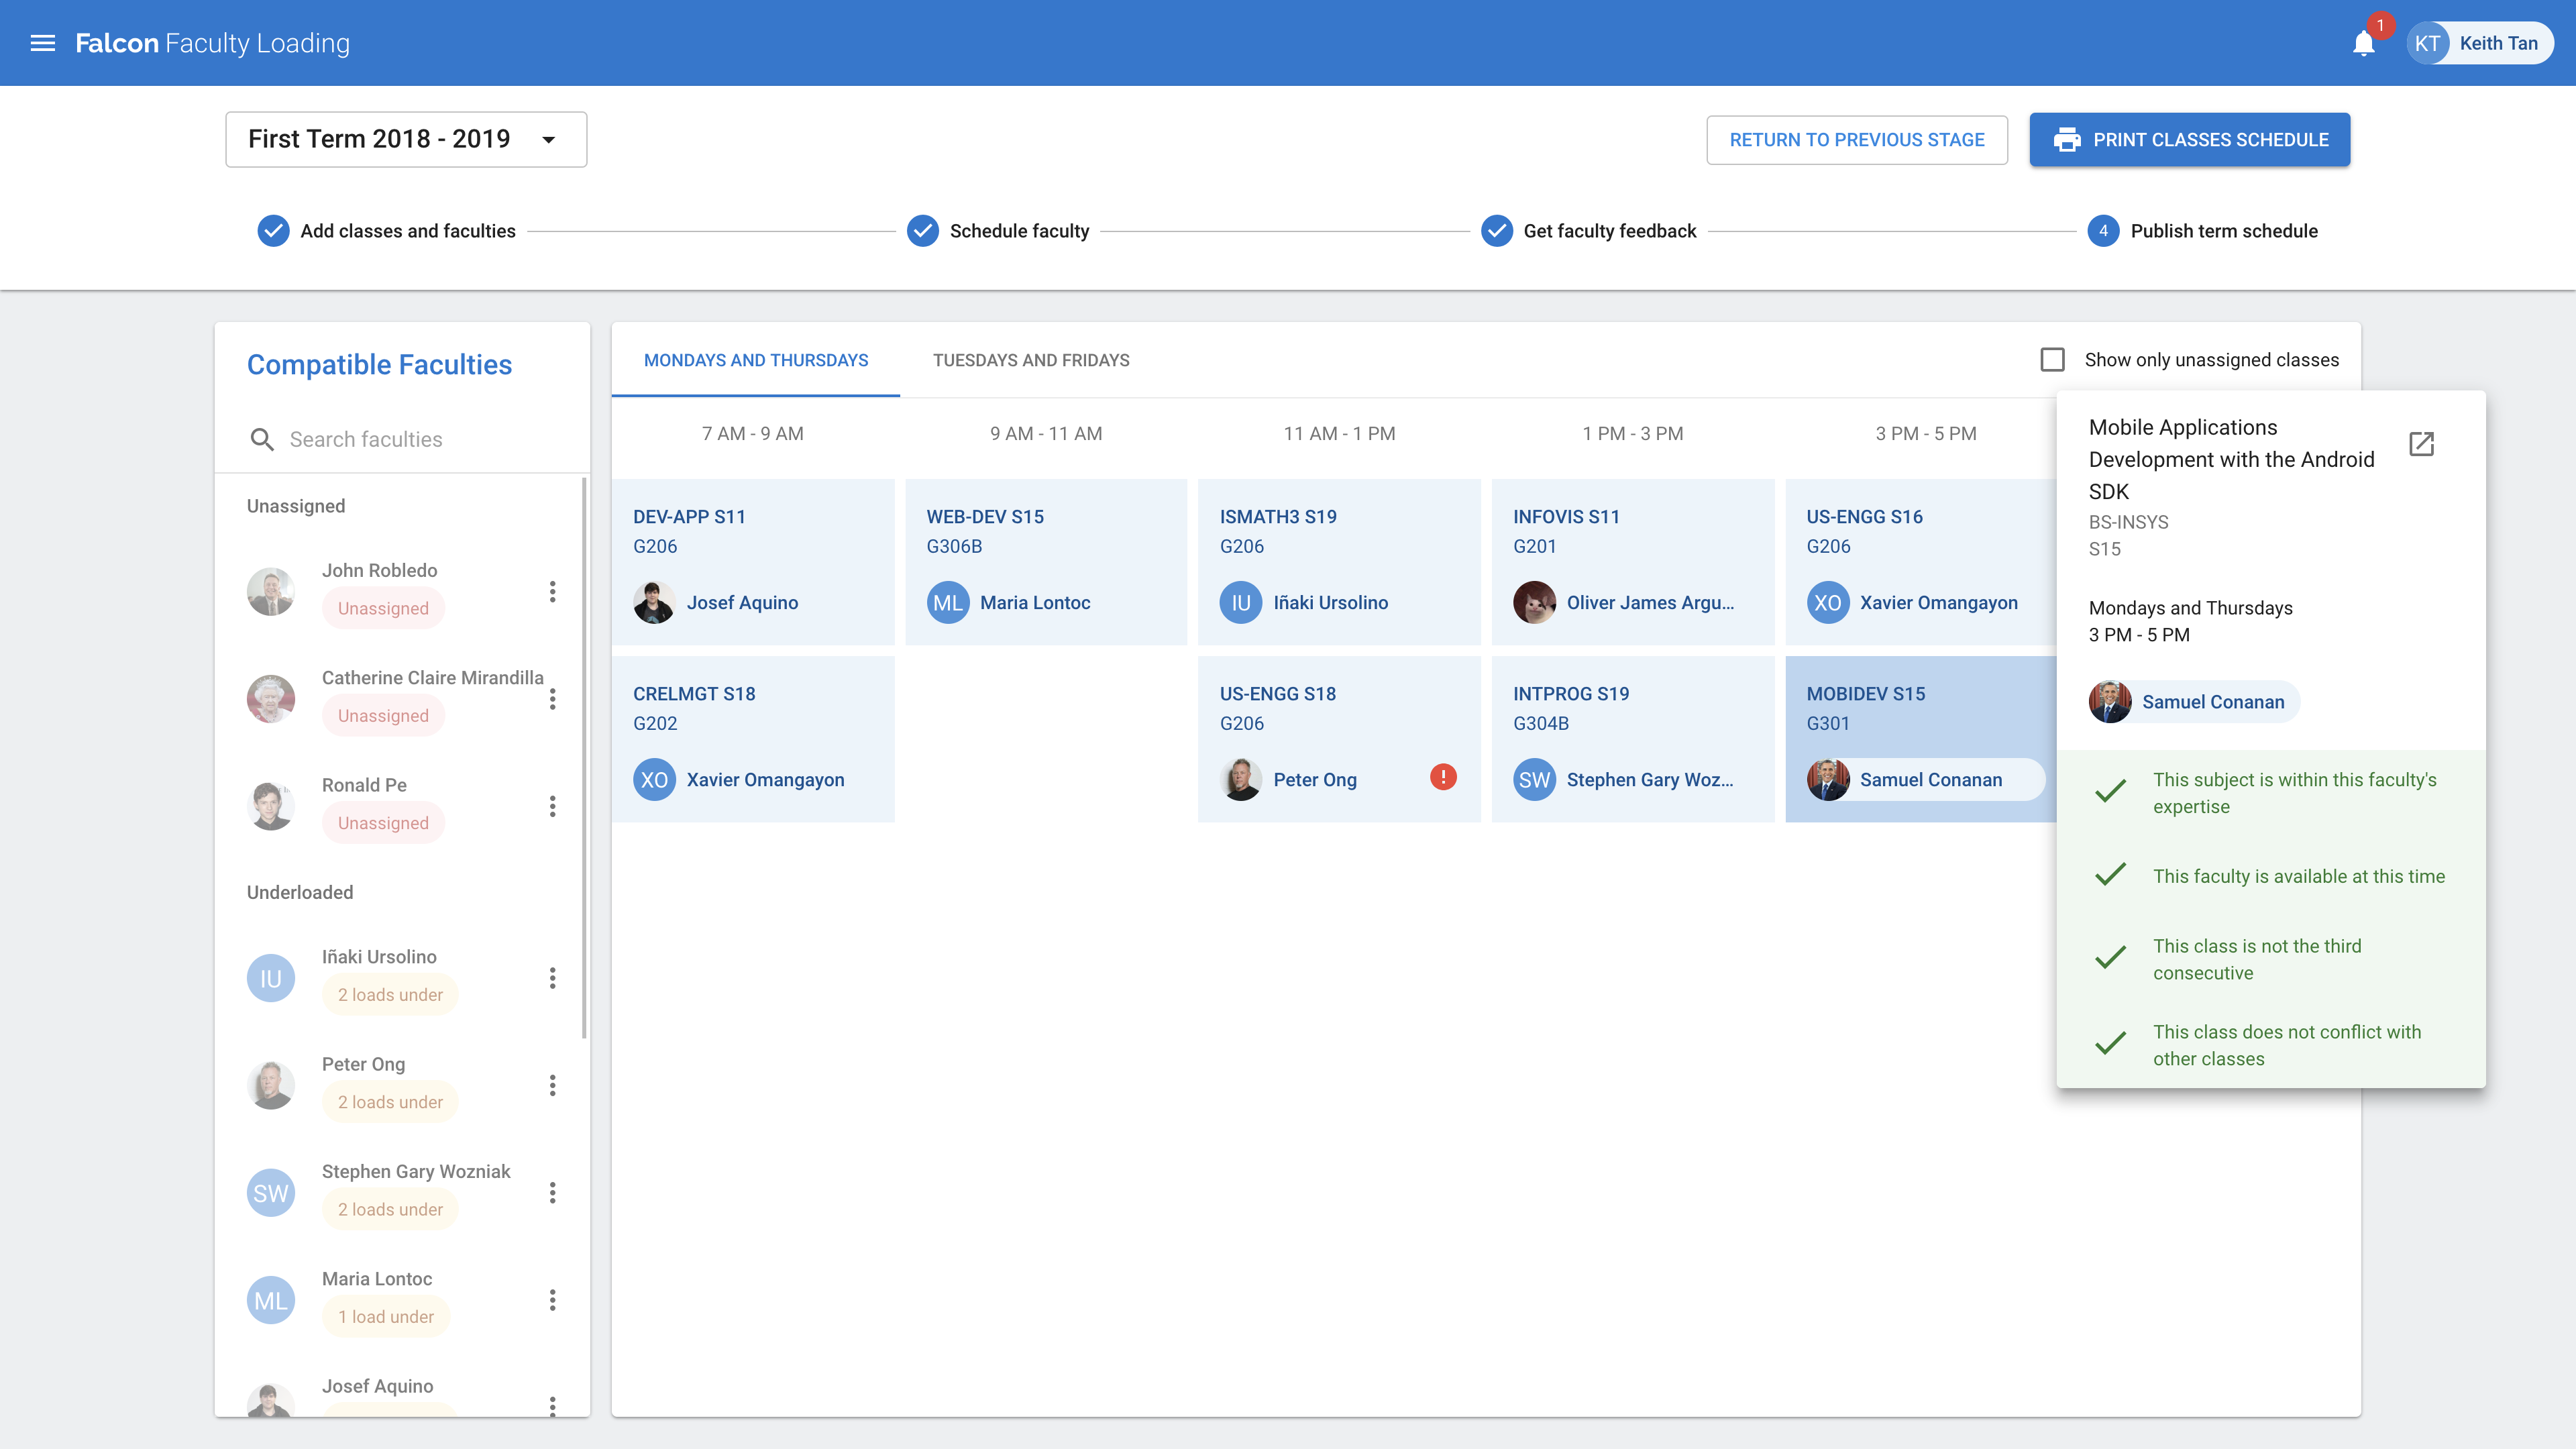
\includegraphics[width=\linewidth]{figures/screen_specifications/faculty_loading_screens/publish_schedule.png}
   \caption{Publish Schedule Screen}
   }
   
   \pagebreak
   
   \subsubsection{Term Switcher Screen}
    
    \field{Screen Name}{Term Switcher}
    
    \field{File Name}{$/pages/FacultyLoading/components/modals/TermModal/index.js$}
    
    \field{Description} {Lets the clerk or associate dean switch between terms they wish to view.}
    
    \field{Layout}{}
    
\makefigure{!ht}{
   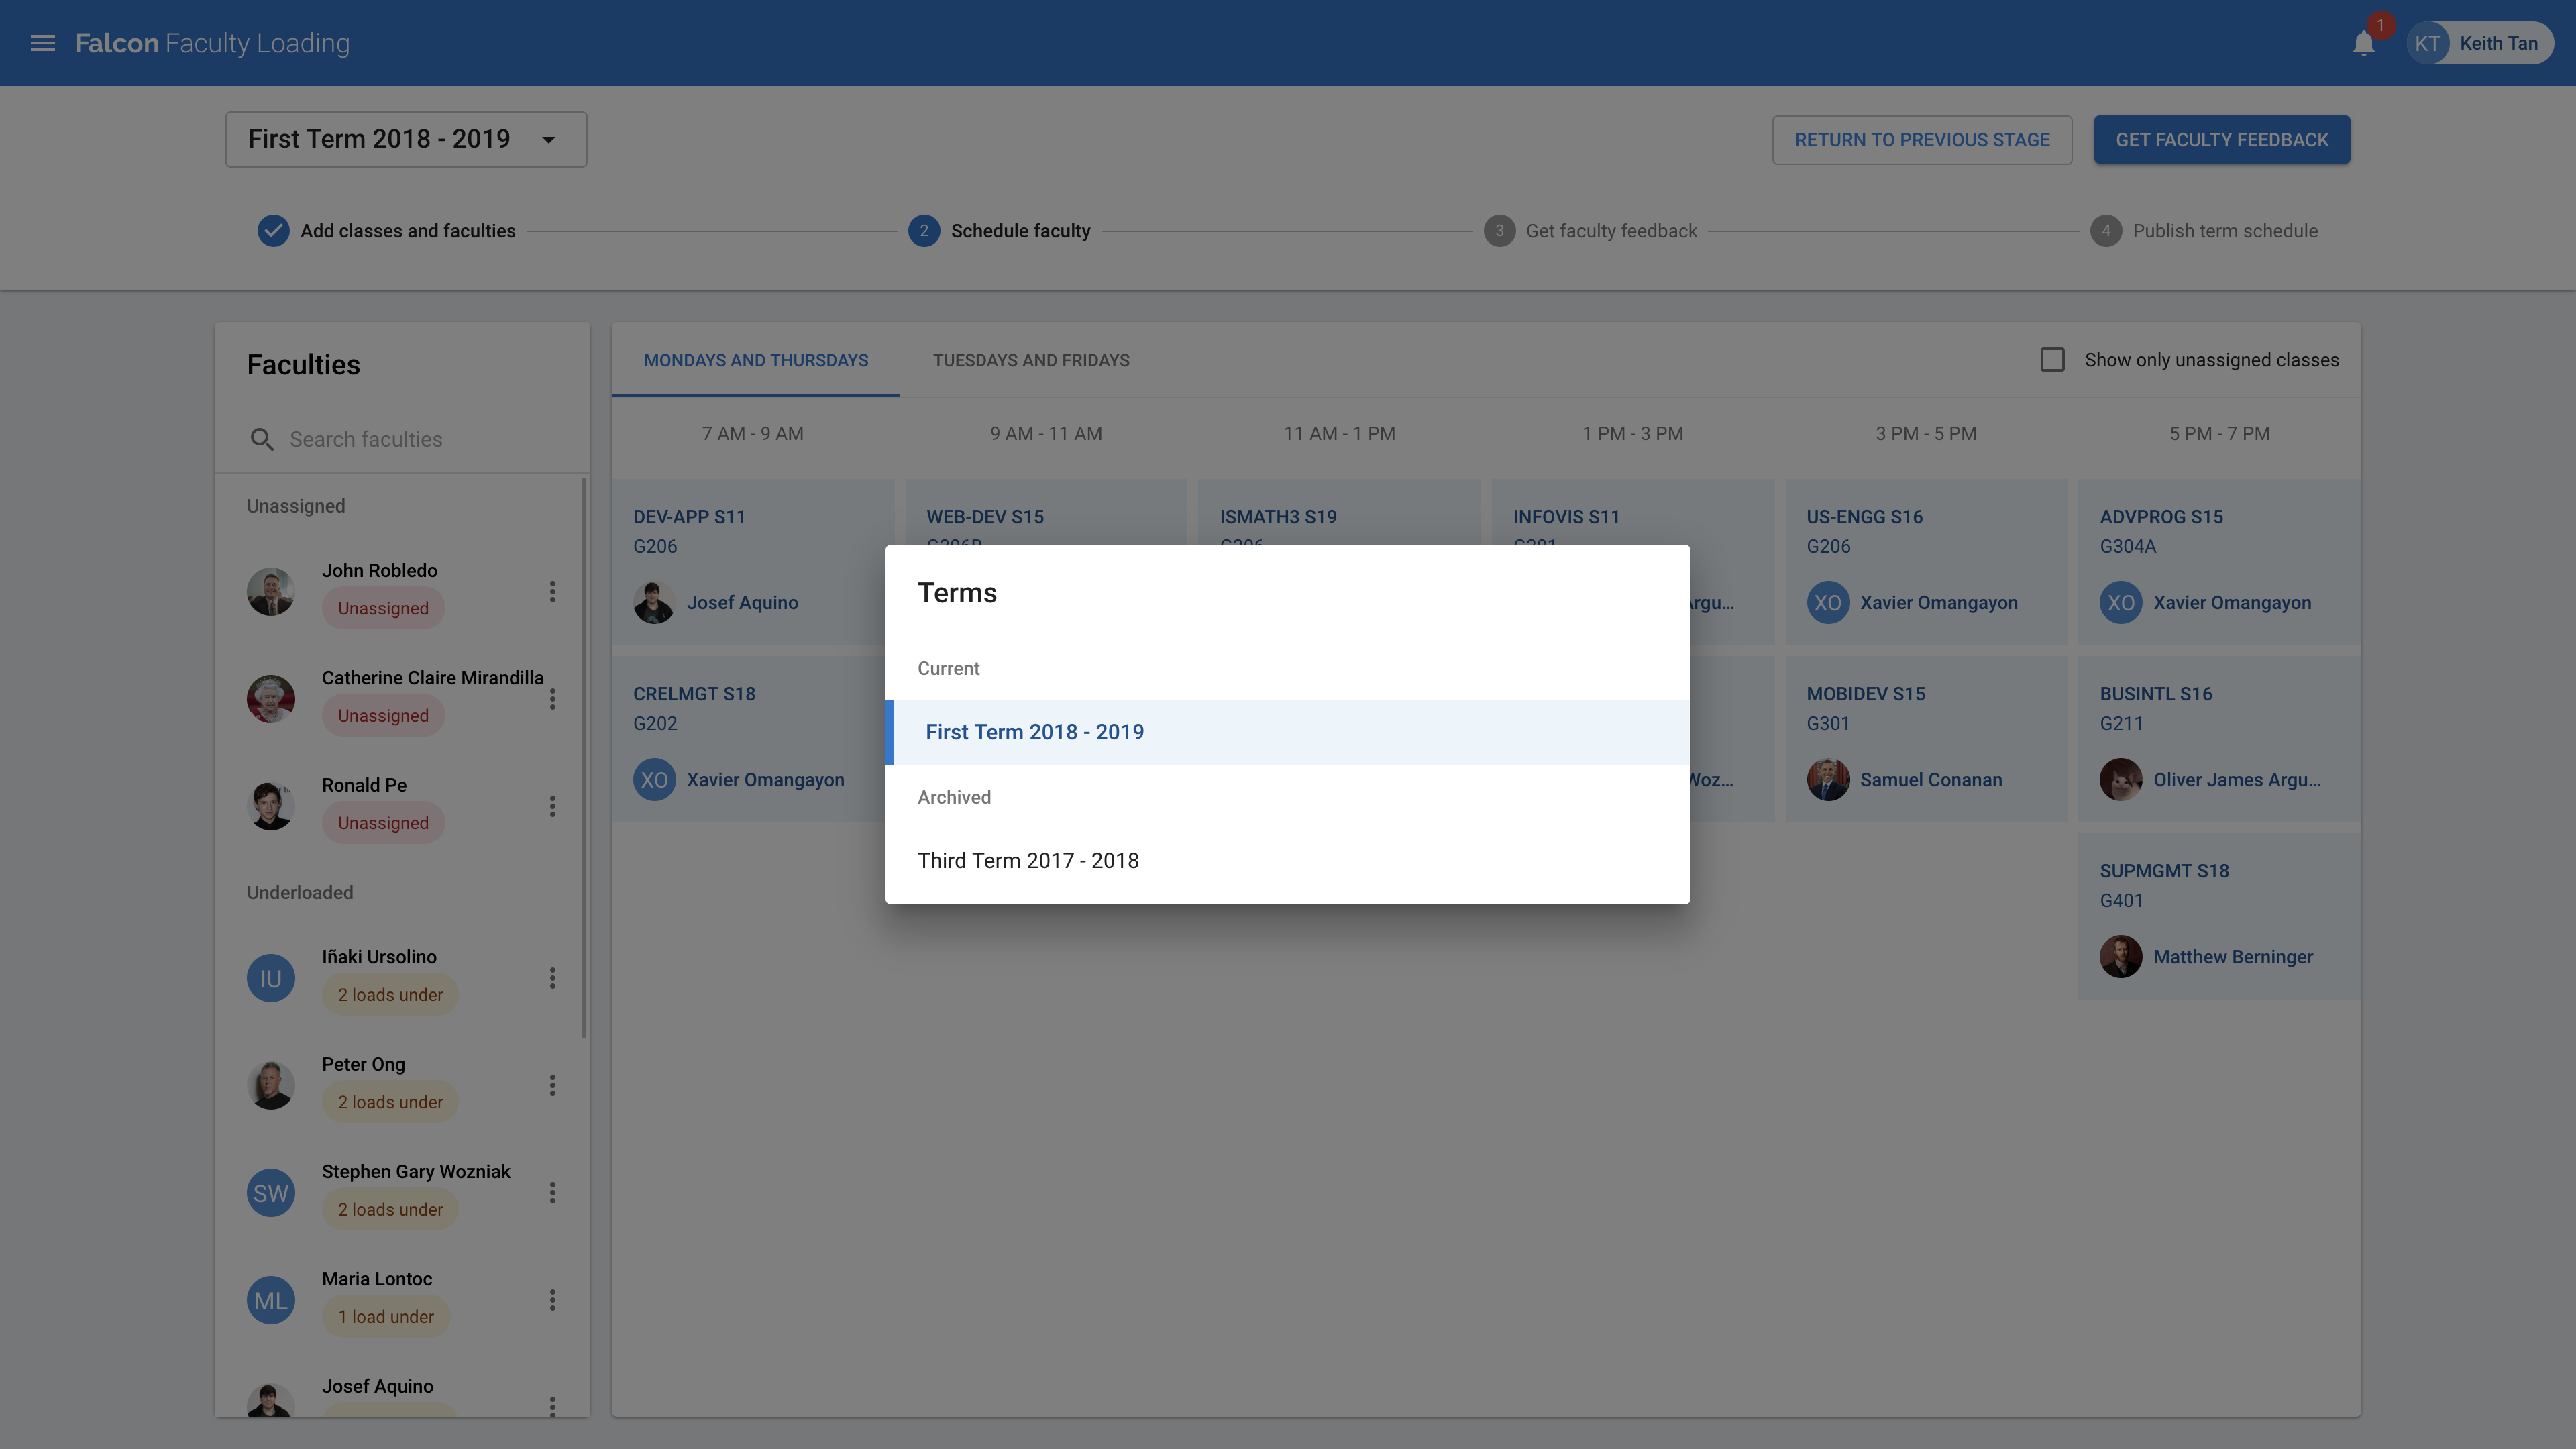
\includegraphics[width=\linewidth]{figures/screen_specifications/faculty_loading_screens/terms_switcher.png}
   \caption{Term Switcher Screen}
   }
   
   \pagebreak
   
   
    \subsubsection{Schedule Print Preview Screen}
    
    \field{Screen Name}{Schedule Print Preview}
    
    \field{File Name}{$/pages/FacultyLoading/components/SchedulePrintPreview/index.js$}
    
    \field{Description} {Displays a preview of the schedule for printing.}
    
    \field{Layout}{}
    
\makefigure{!ht}{
   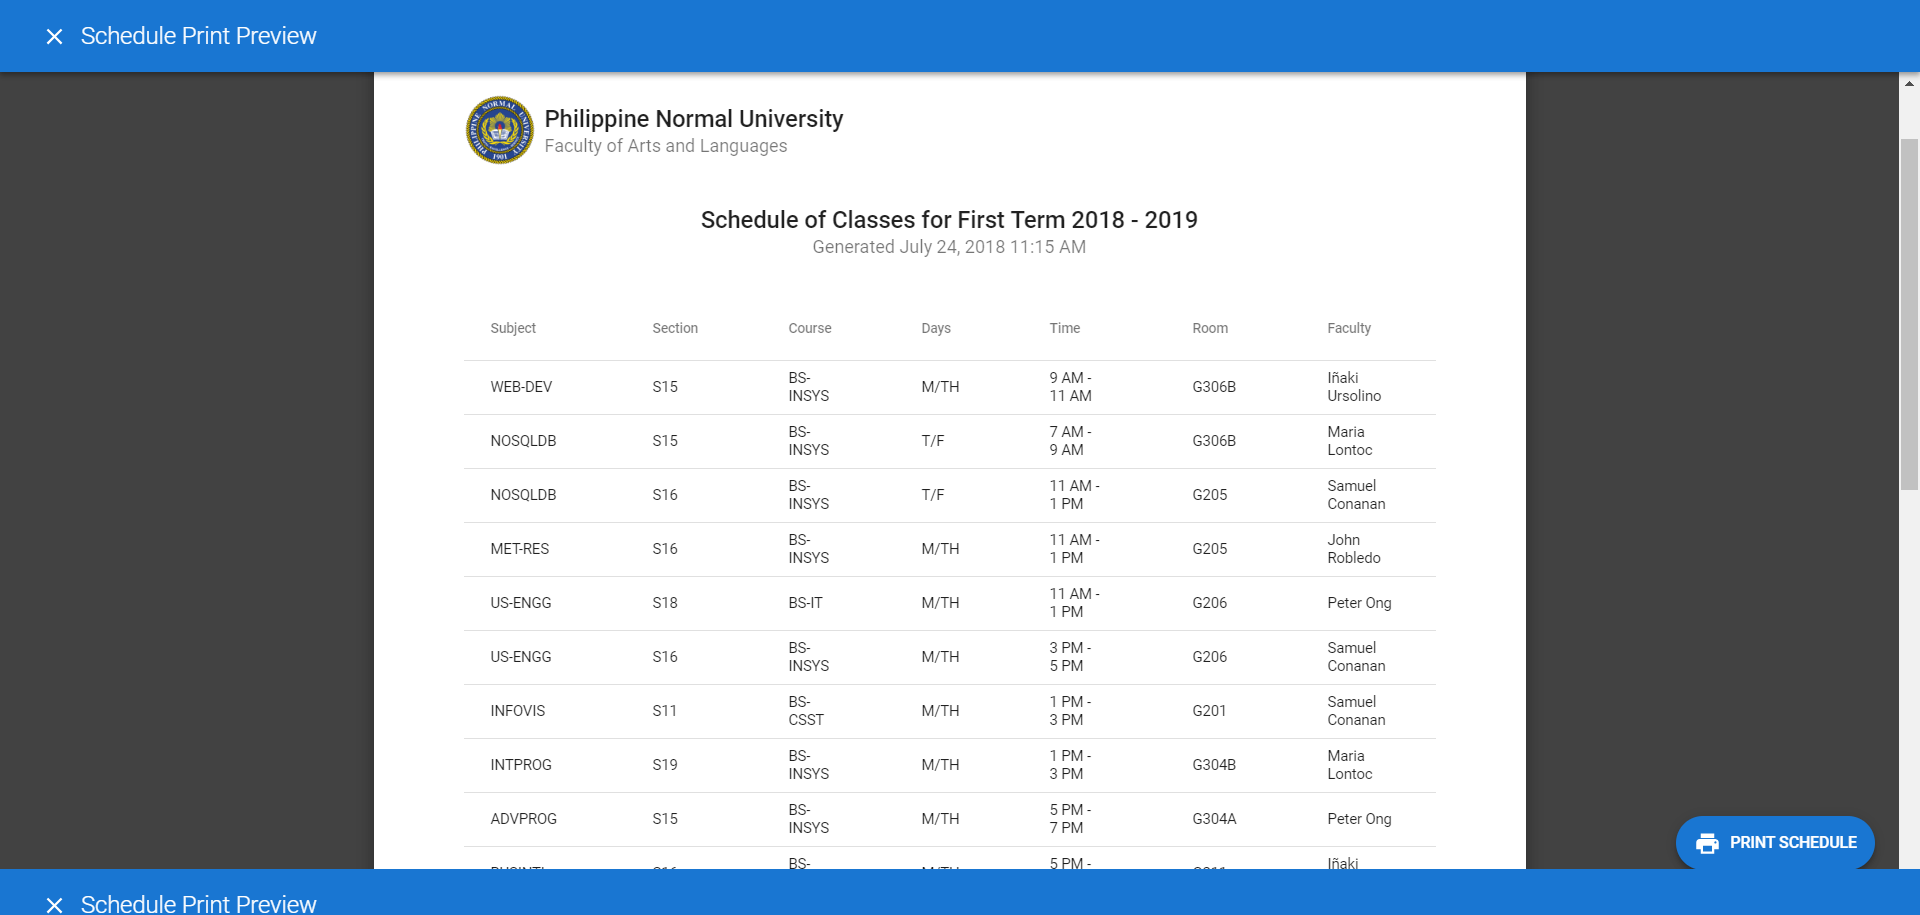
\includegraphics[width=\linewidth]{figures/screen_specifications/faculty_loading_screens/schedule_print.png}
   \caption{Schedule Print Preview Screen}
   }
   
   \pagebreak
   
   
   \subsubsection{Time Availability}
    
    \field{Screen Name}{Time Availability}
    
    \field{File Name}{$/pages/FacultyLoading/components/modals/FacultyAvailabilityModal/index.js$}
    
    \field{Description} {Displays the days and times of the faculty members' availability.}
    
    \field{Layout}{}
    
\makefigure{!ht}{
   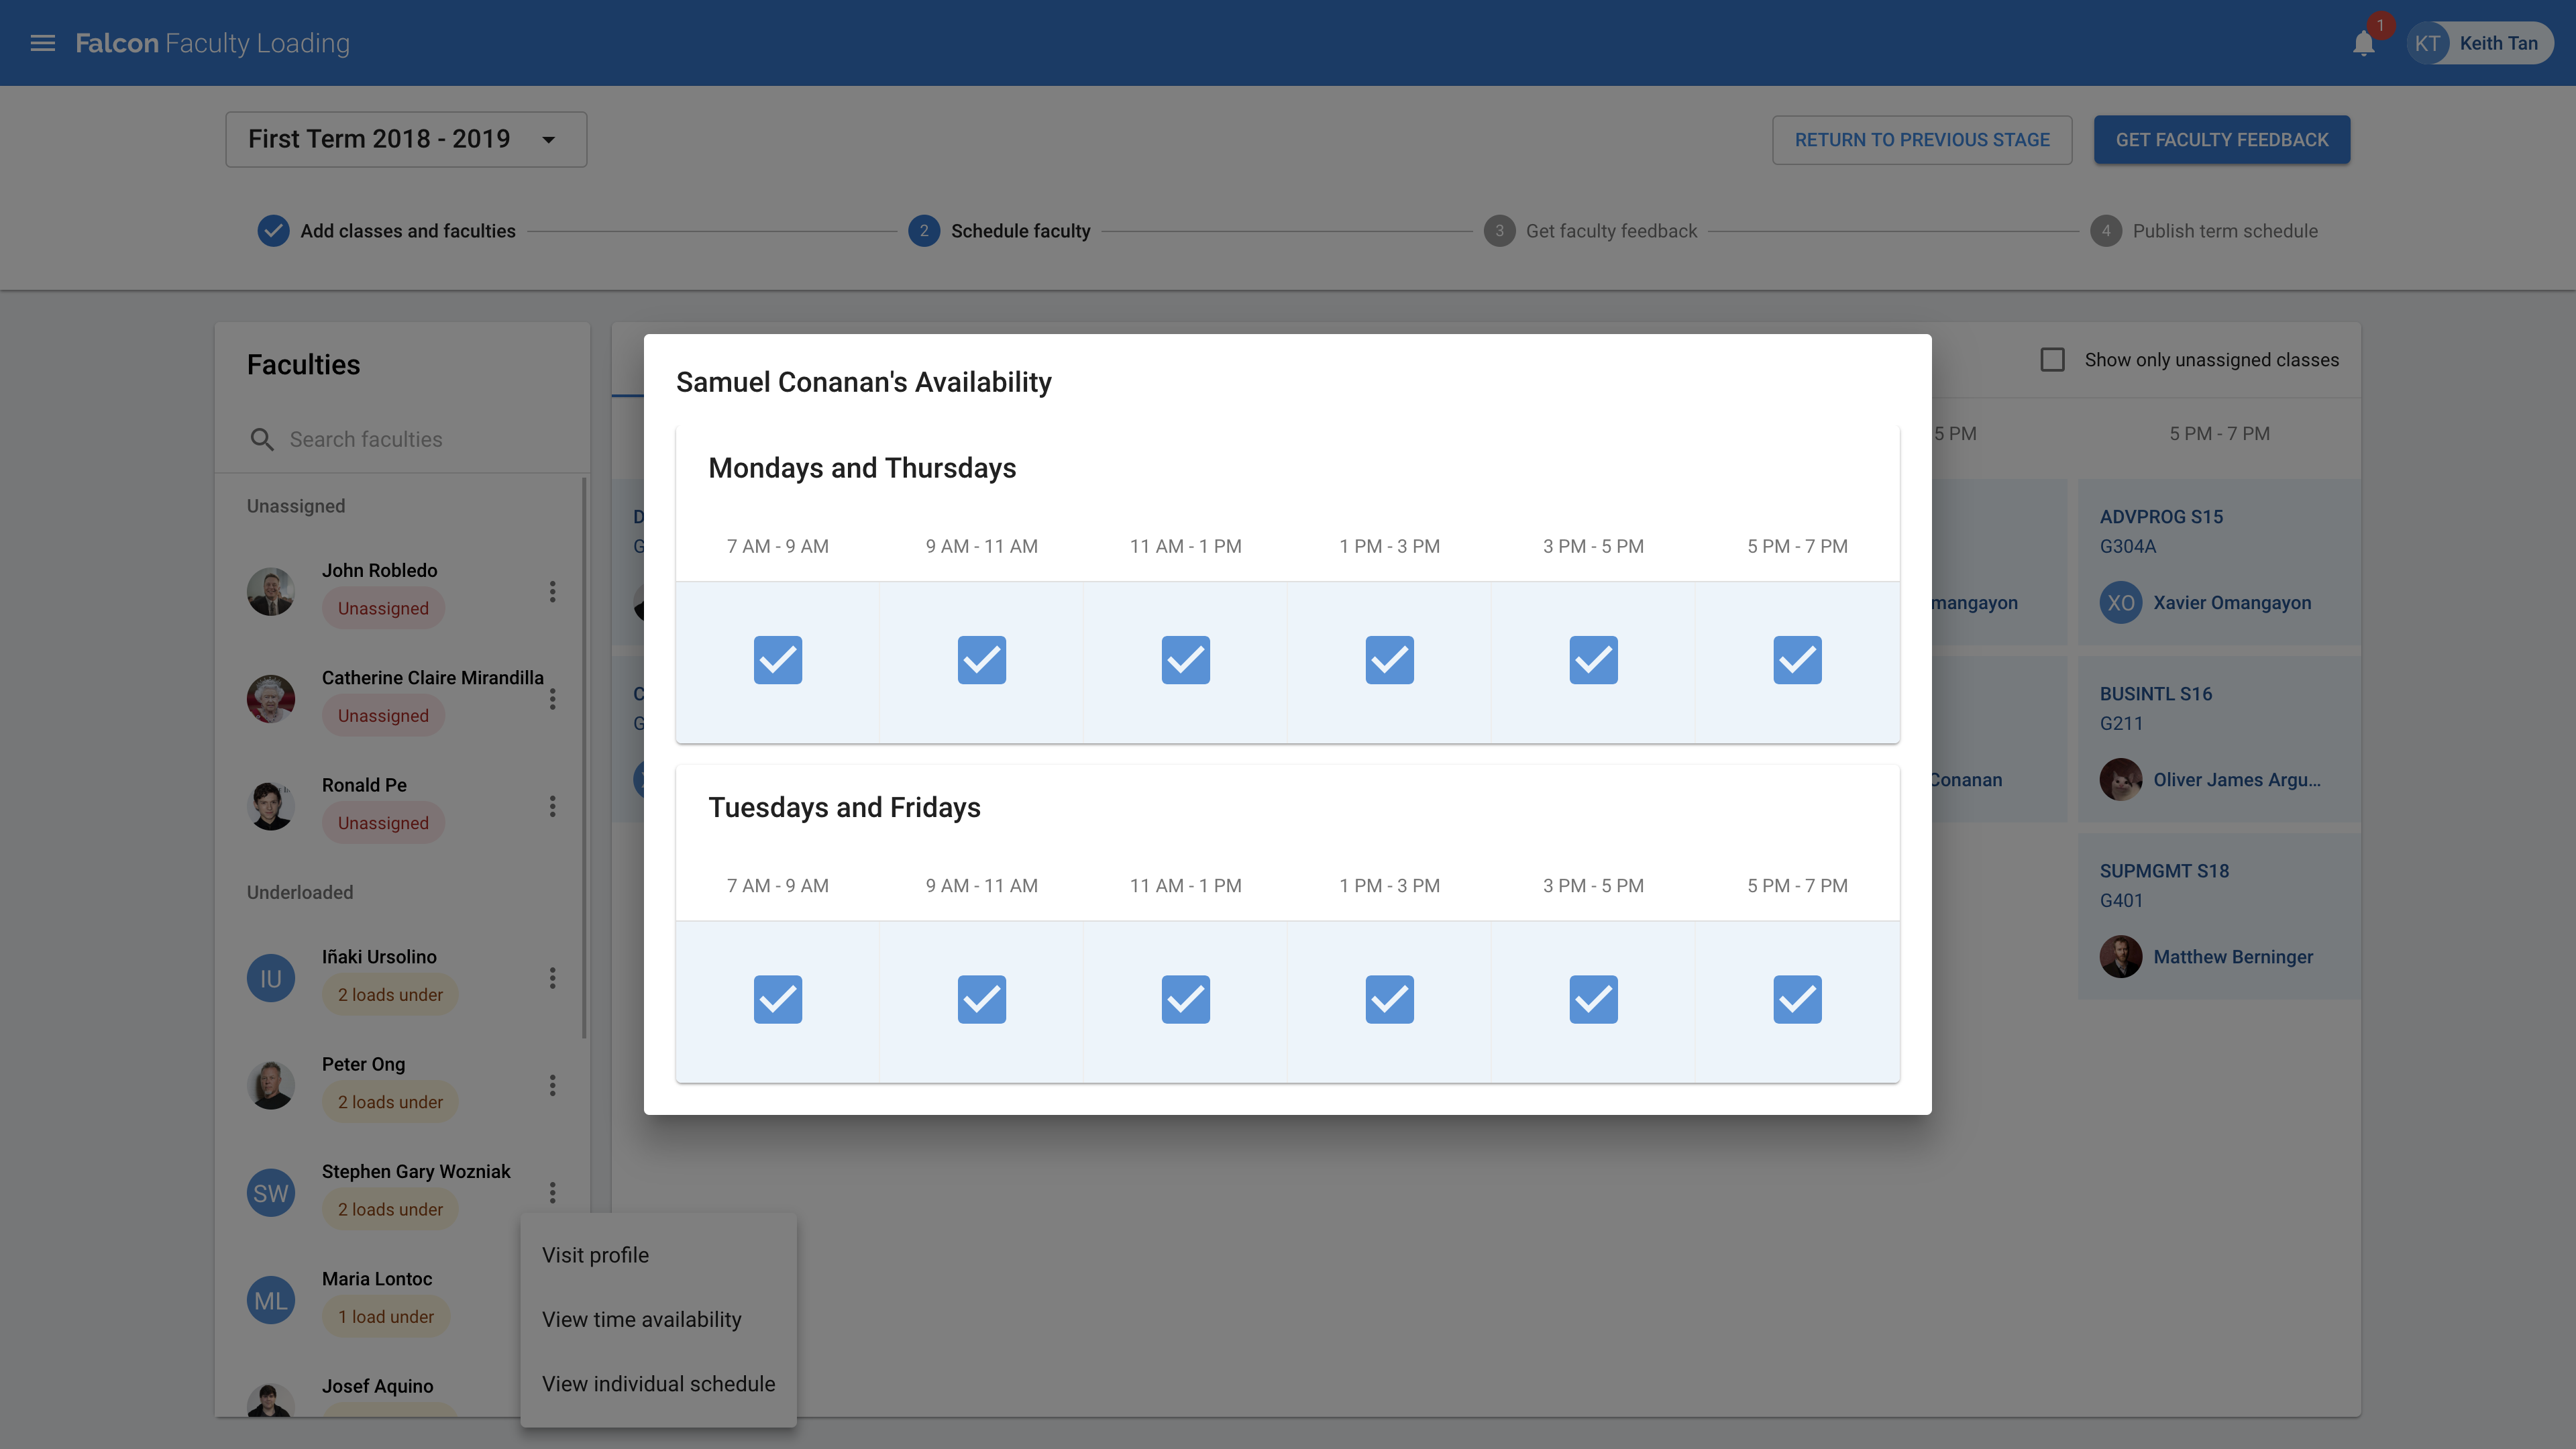
\includegraphics[width=\linewidth]{figures/screen_specifications/faculty_loading_screens/time_availability.png}
   \caption{Time Availability Screen}
   }
   
   \pagebreak
   
    \subsubsection{Subjects Overview}
    
    \field{Screen Name}{Subjects Overview}
    
    \field{File Name}{$/pages/Subjects/index.js$}
    
    \field{Description} {Displays the list of subjects with it's details, such as basic information and a list of expert faculties.}
    
    \field{Layout}{}
    
\makefigure{!ht}{
   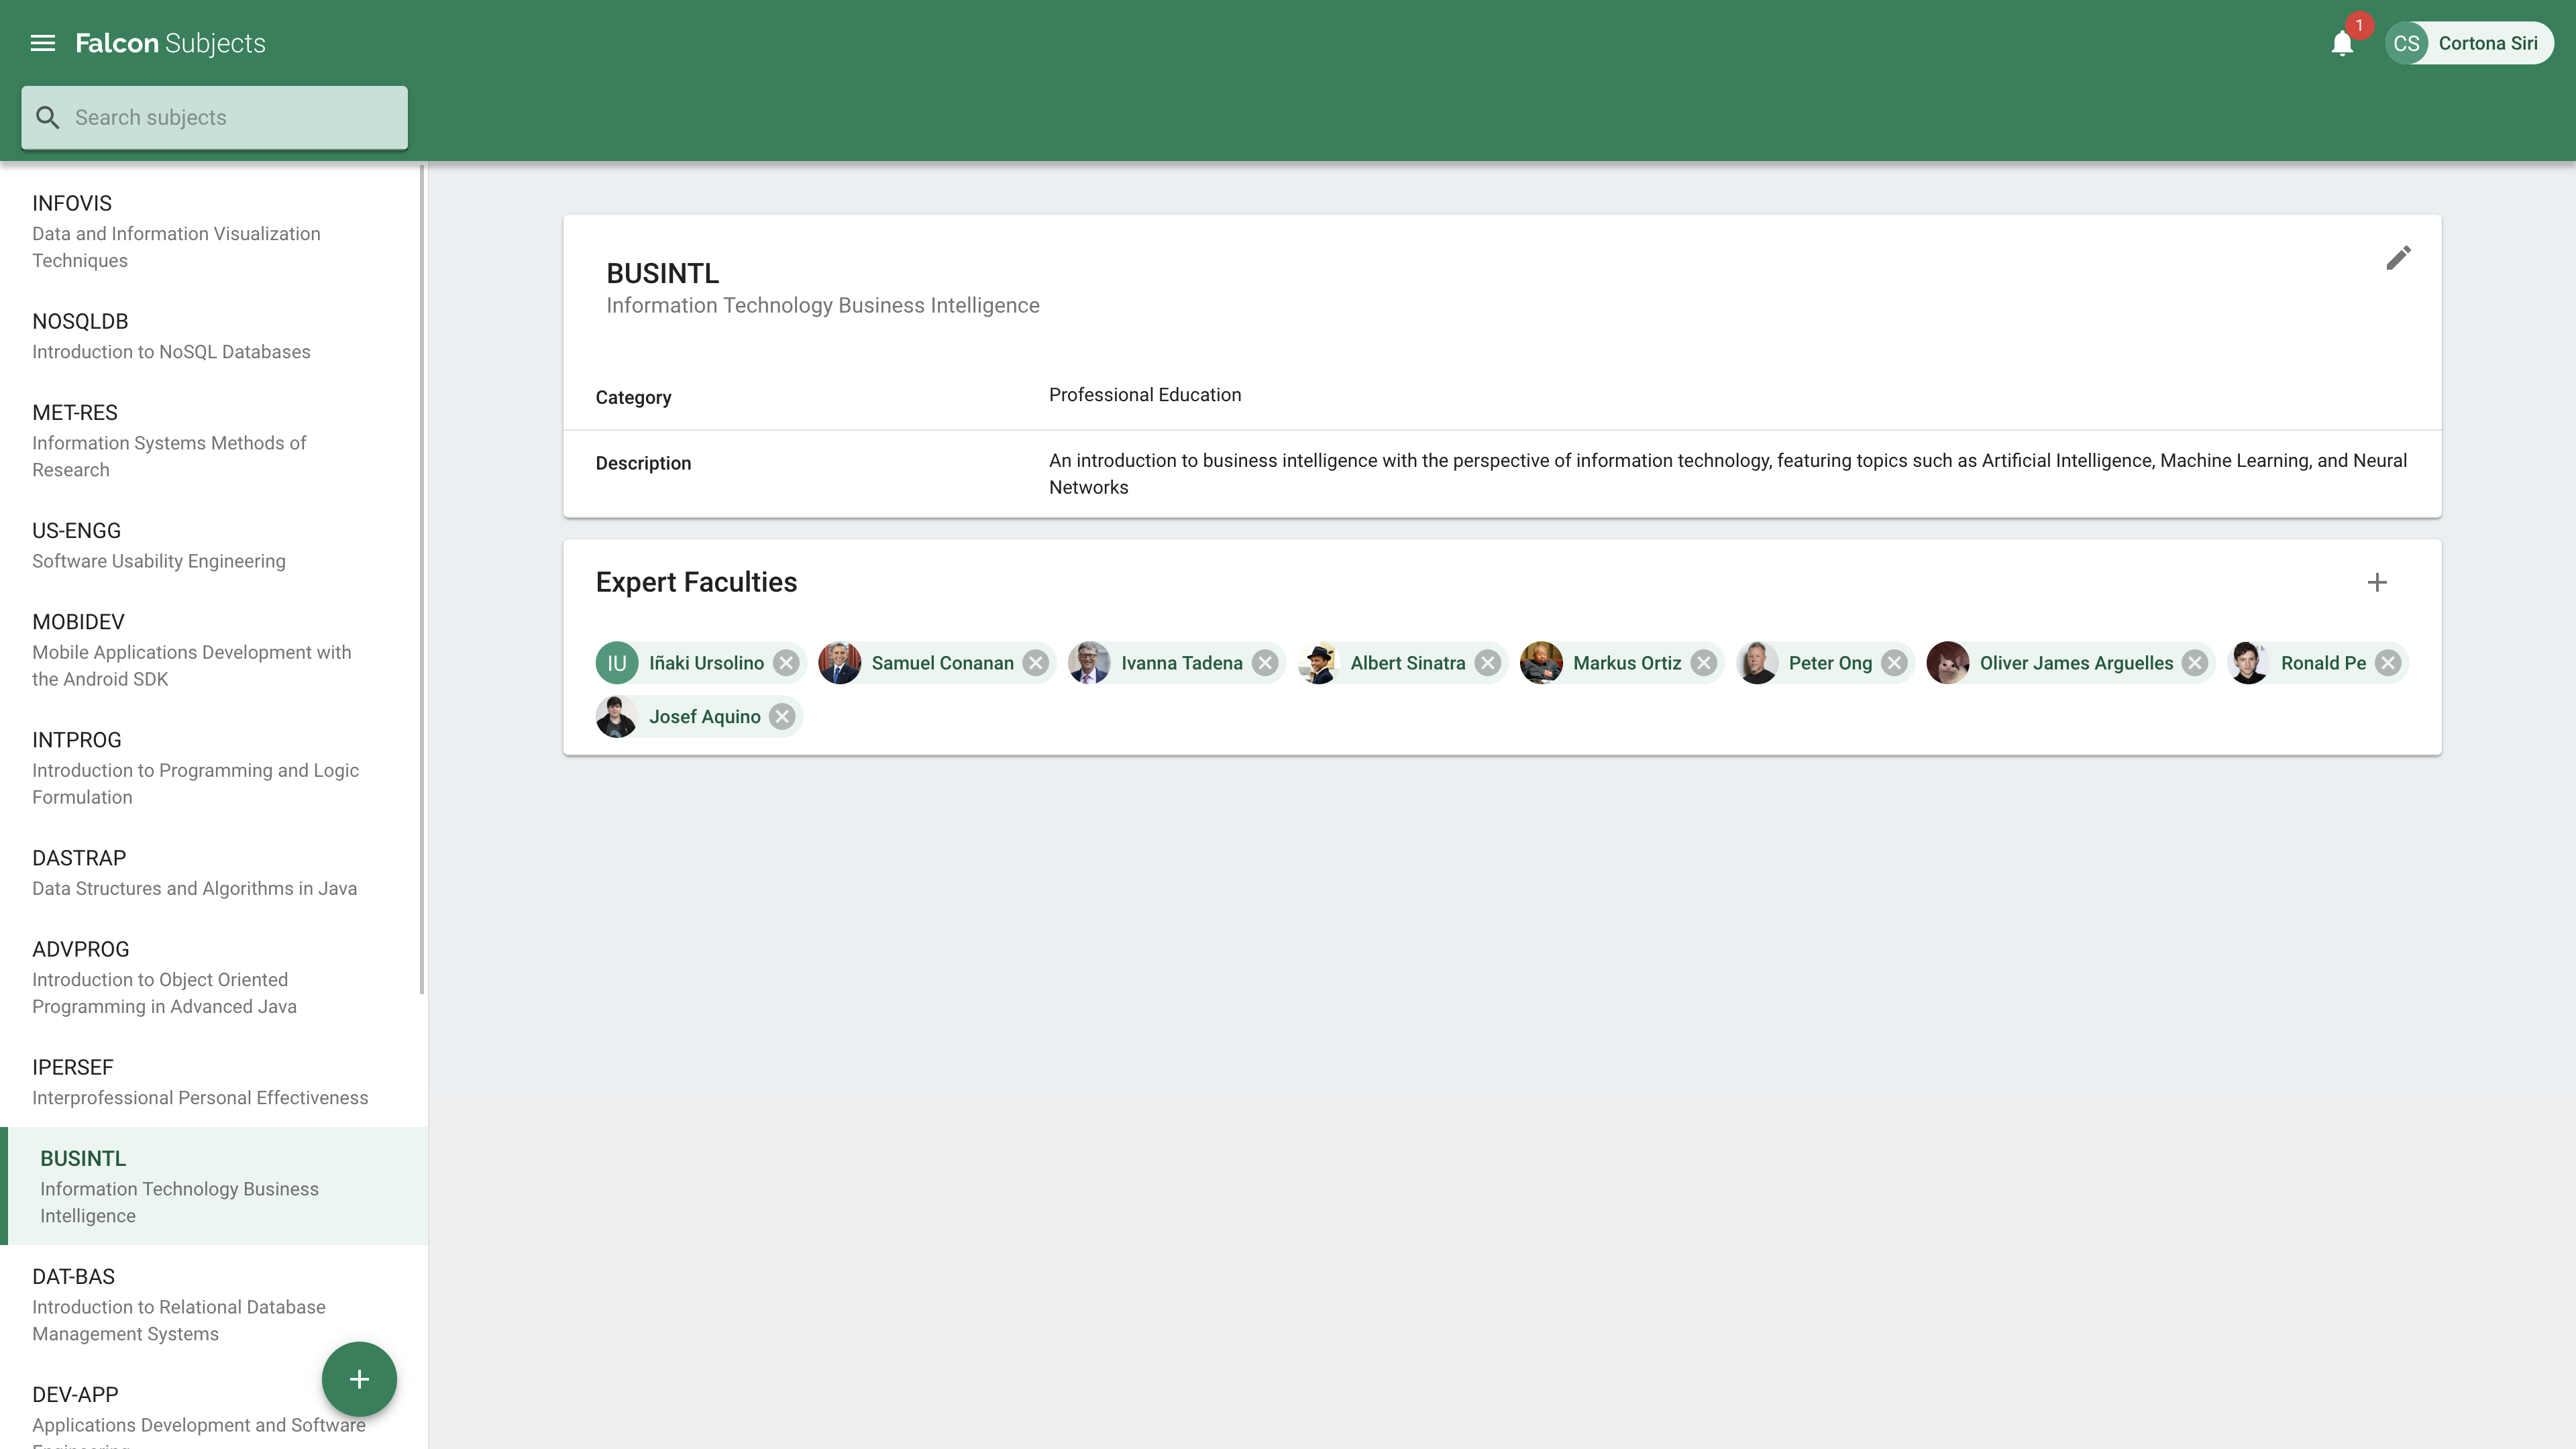
\includegraphics[width=\linewidth]{figures/screen_specifications/faculty_loading_screens/subjects_overview.png}
   \caption{Subjects Overview Screen}
   }
   
   \pagebreak
   
   
    \subsubsection{Individual Schedule}
    
    \field{Screen Name}{Individual Schedule}
    
    \field{File Name}{$/pages/FacultyLoading/components/modals/FacultyScheduleModal/index.js$}
    
    \field{Description} {Displays the schedule of each individual faculty member.}
    
    \field{Layout}{}
    
\makefigure{!ht}{
   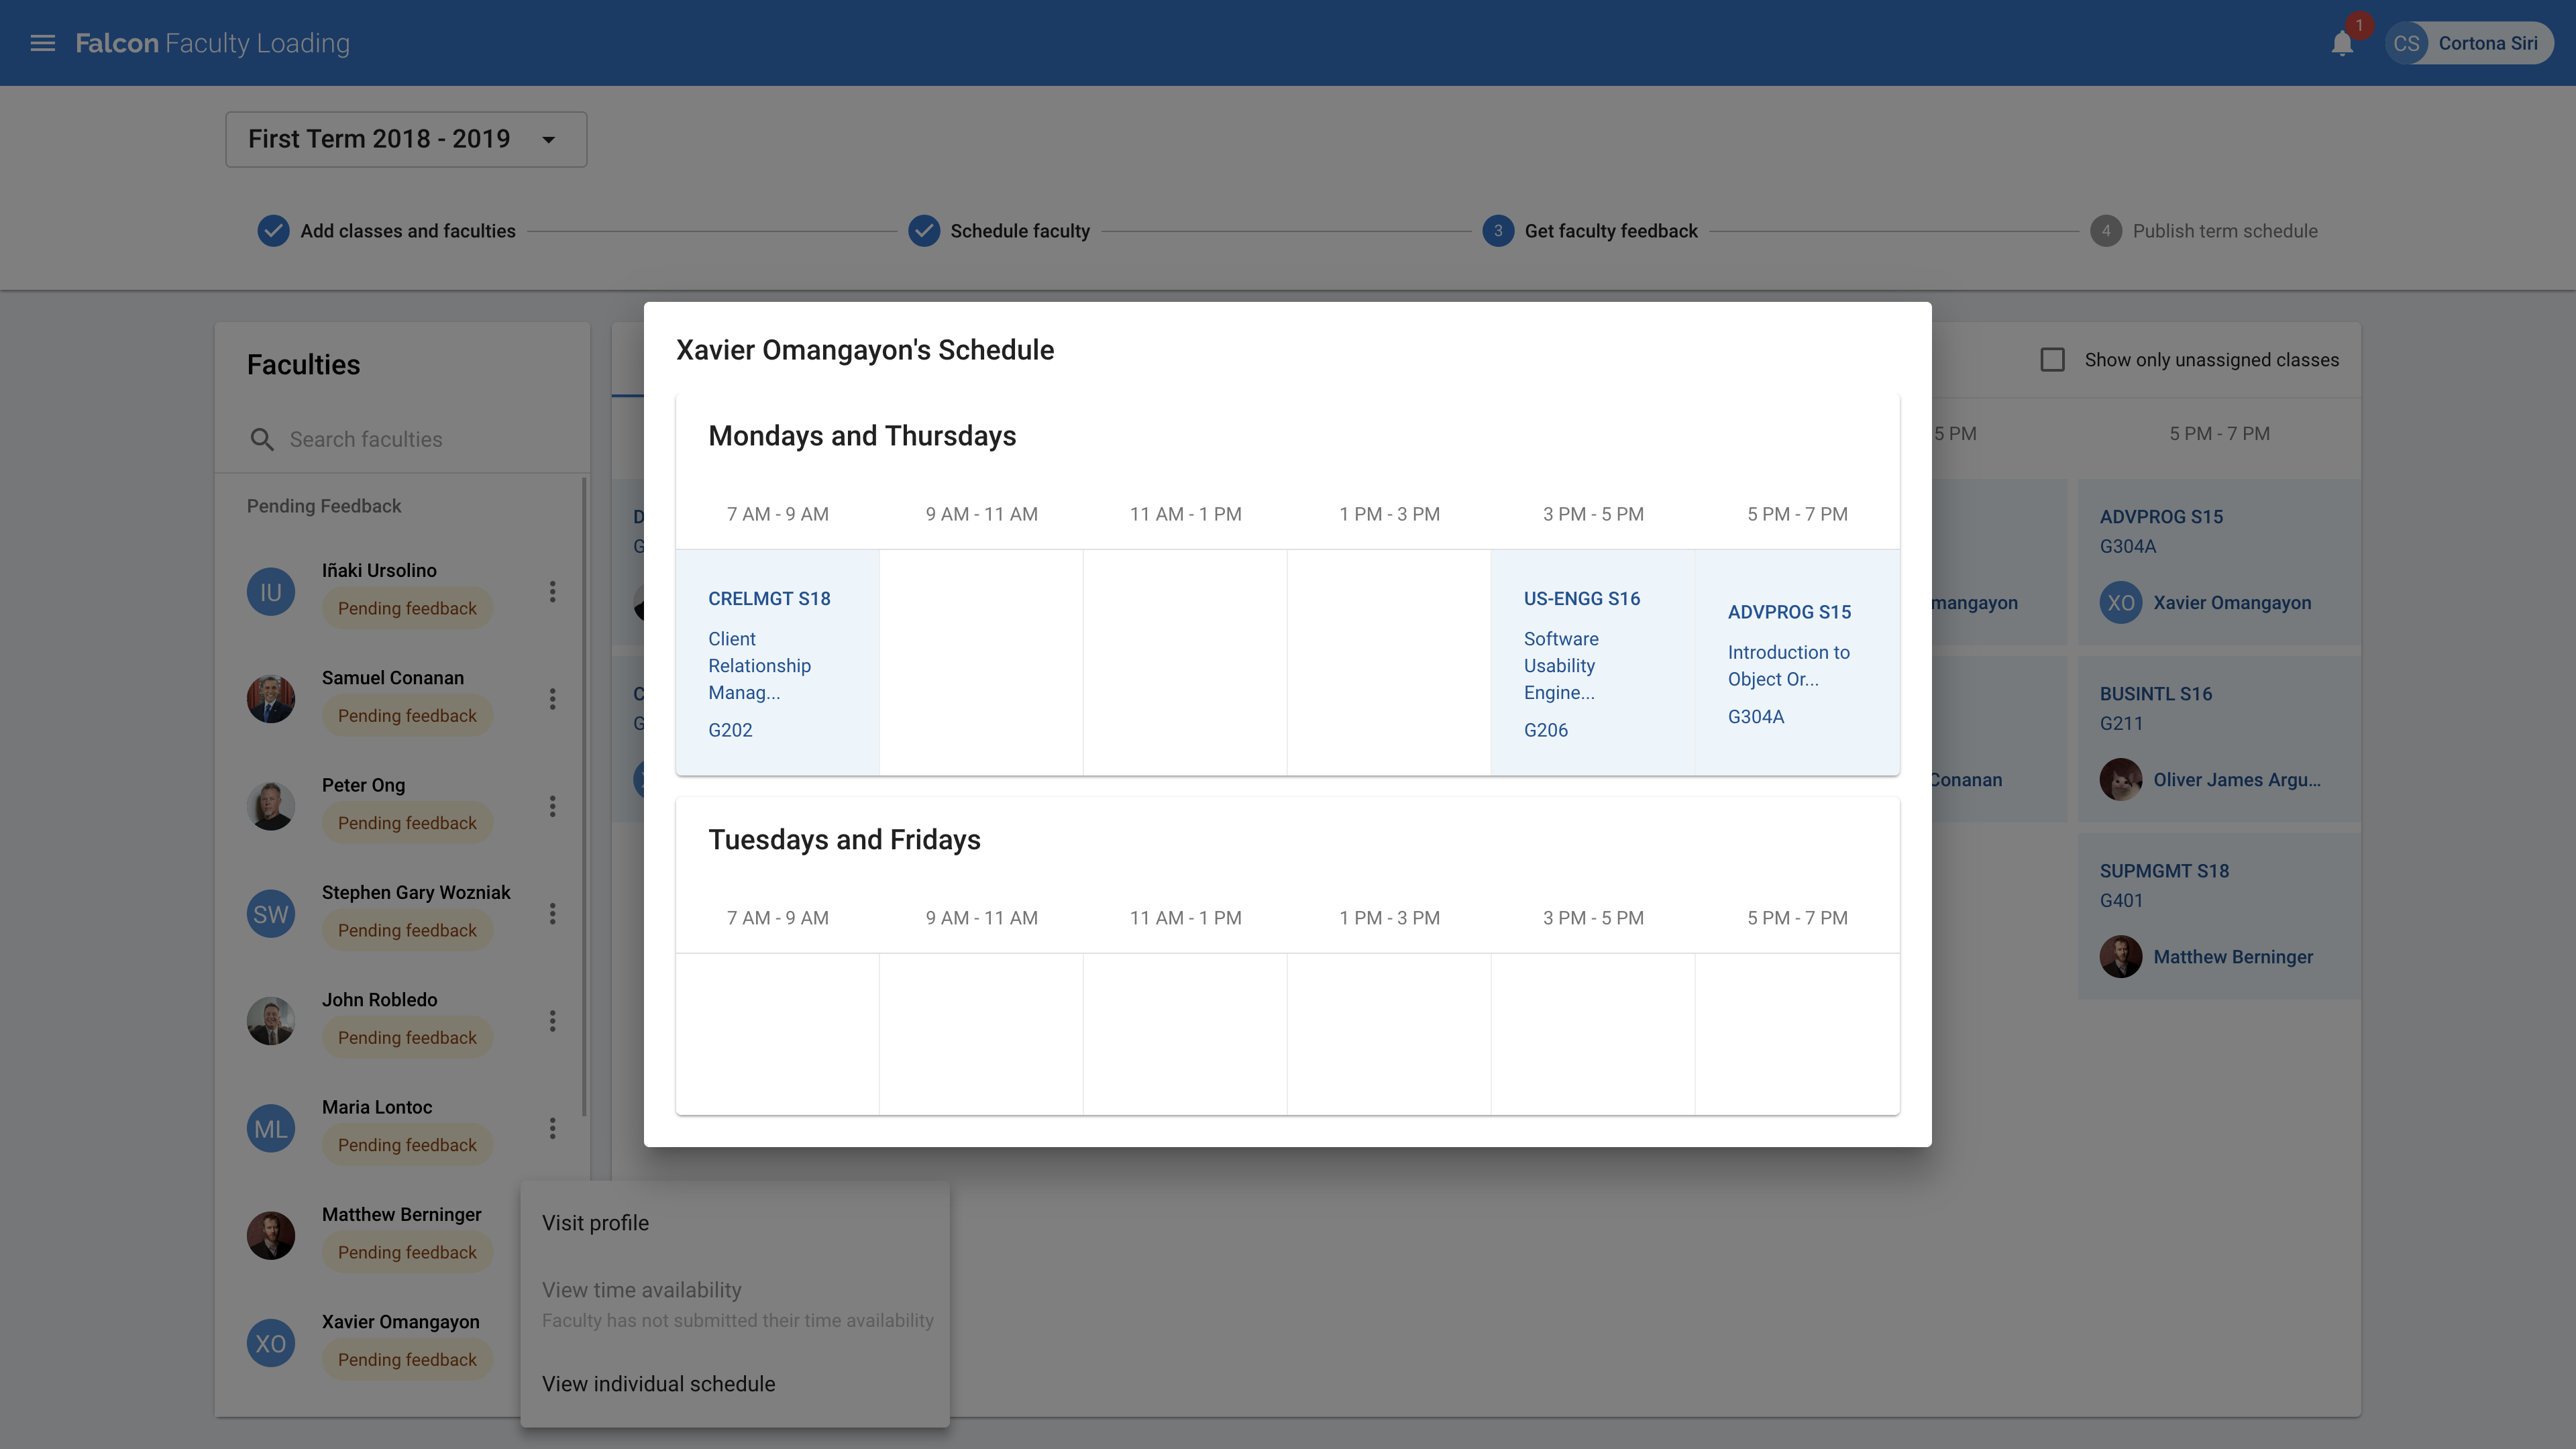
\includegraphics[width=\linewidth]{figures/screen_specifications/faculty_loading_screens/individual_schedule.png}
   \caption{Individual Schedule Screen}
   }
   
   \pagebreak
   
   
    \subsubsection{Schedule Print Preview}
    
    \field{Screen Name}{Schedule Print Preview}
    
    \field{File Name}{$/pages/FacultyLoading/components/SchedulePrintPreview/index.js$}
    
    \field{Description} {Displays the print preview for the schedules before printing.}
    
    \field{Layout}{}
    
\makefigure{!ht}{
   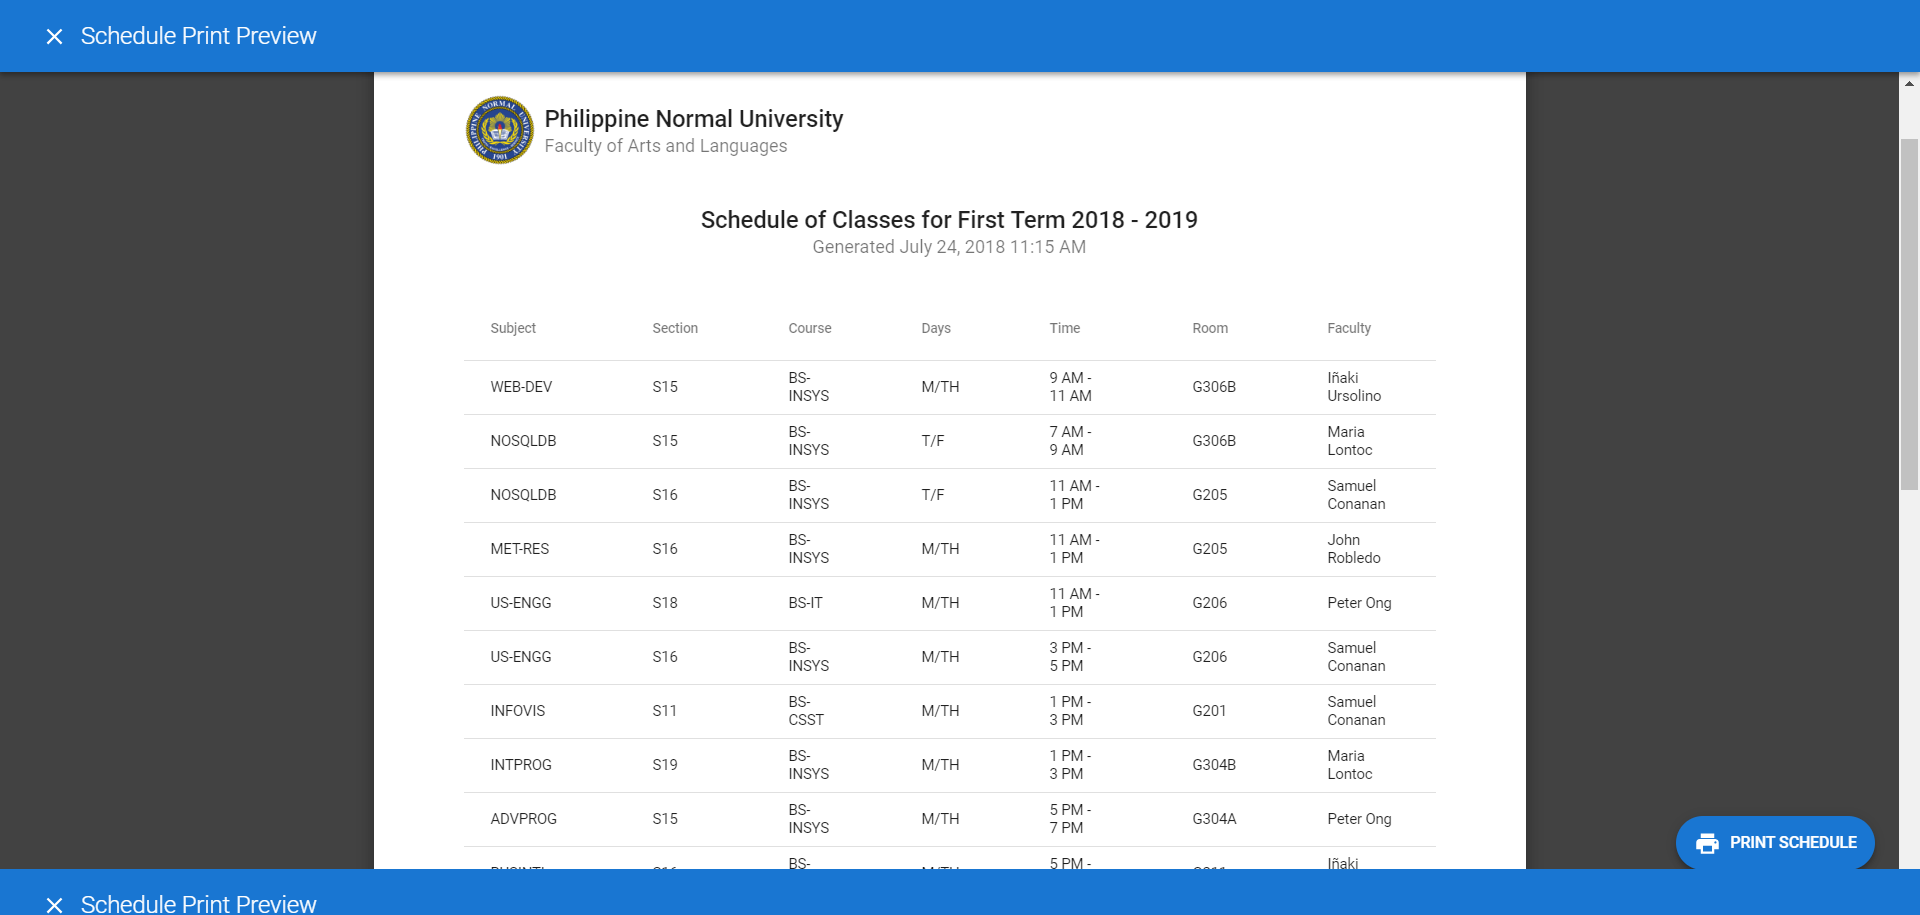
\includegraphics[width=\linewidth]{figures/screen_specifications/faculty_loading_screens/schedule_print.png}
   \caption{Schedule Print Preview Screen}
   }
   
   \pagebreak
   
   
   
   \subsection{My Schedule}
    
    \subsubsection{My Schedule Feedback Screen}
    
    \field{Screen Name}{My Schedule Feedback}
    
    \field{File Name}{$/pages/FacultyLoading/index.js$}
    
    \field{Description} {Displays the schedule of the faculty during the get feedback stage of creating a term schedule. This allows the faculty to accept or reject their given schedule and send feedback for the schedule.}
    
    \field{Layout}{}
    
\makefigure{!ht}{
   \includegraphics[width=\linewidth]{figures/screen_specifications/faculty_loading_screens/myschedule_feedback.png}
   \caption{My Schedule Feedback Screen}
   }
   
   \pagebreak
   
   
   \subsubsection{My Schedule Publish Screen}
    
    \field{Screen Name}{My Schedule Publish}
    
    \field{File Name}{$/pages/FacultyLoading/index.js$}
    
    \field{Description} {Displays the schedule of the faculty after the term schedule has been published.}
    
    \field{Layout}{}
    
\makefigure{!ht}{
   \includegraphics[width=\linewidth]{figures/screen_specifications/faculty_loading_screens/myschedule_publish.png}
   \caption{My Schedule Publish Screen}
   }
   
   \pagebreak
   
   
   
   
    
\section{Form Specifications}

    \subsection{Faculty Profile}
    
    \subsubsection{Create User}
    
    \field{Form Name}{Create User}
    
    \field{Description}{For users to enter the basic information of their profile.}
    
    \field{Prepared by}{Clerk}
    
    \field{Volume and Frequency}{Created when a new faculty joins FAL.}
    
    \field{Layout}{}
    
    \pagebreak
    
\makefigure{!ht}{
   \includegraphics[width=\linewidth]{figures/form_specifications/create_user.png}
   \caption{Create User Screen}
}
    \pagebreak
    
    
    \subsubsection{Set Faculty}
    \field{Form Name} {Set Faculty}
    
    \field{Description}{For the faculty to input additional information into their profile.}
    
    \field{Prepared by} {Clerk}
    
    \field{Volume and Frequency}{Created when a new faculty joins FAL.}
    
    \field{Layout}{}
    
\makefigure{ht}{
   \includegraphics[width=\linewidth]{figures/form_specifications/set_faculty_details.png}
   \caption{Set Faculty Details Screen}
   }
   
   \pagebreak
    
    \subsubsection{Review Faculty}
    \field{Form Name}{Review Faculty}
    
    \field{Description}{For users review the information they entered into the profile.}
    
    \field{Prepared by}{Clerk}
    
    \field{Volume and Frequency}{Created when a new faculty joins FAL.}
    
    \field{Layout}{}
    
\makefigure{!ht}{
   \includegraphics[width=\linewidth]{figures/form_specifications/review_details.png}
   \caption{Review Faculty Screen}
   }
   
   \pagebreak
    
    \subsubsection{Update Faculty}
    \field{Form Name}{Update Faculty}
    
    \field{Description}{For users to update the information in the faculty profile.}
    
    \field{Prepared by}{Clerk}
    
    \field{Volume and Frequency}{When information on the faculty profile needs to be updated}
    
    \field{Layout}{}
    
\makefigure{!ht}{
   \includegraphics[width=\linewidth]{figures/form_specifications/update_faculty.png}
   \caption{Update Faculty Screen}
   }
   \pagebreak
    
    \subsubsection{Add/Update Degree}
    \field{Form Name}{Add/Update Degree}
    
    \field{Description}{For users to add a new degree or update the details of an existing degree.}
    
    \field{Prepared by}{Clerk}
    
    \field{Volume and Frequency}{Added when the faculty earns a new degree, or when faculty has requested to add or update their degree.}
    
    \field{Layout}{}
    
\makefigure{!ht}{
   \includegraphics[width=\linewidth]{figures/form_specifications/add_degree.png}
   \caption{Add/Update Degree Screen}
   }
    
    \pagebreak
    
    \subsubsection{Add/Update Recognition}
    \field{Form Name}{Add/Update Recognition}
    
    \field{Description}{For the clerk to add a new degree or update the details of an existing degree.}
    
    \field{Prepared by}{Clerk}
    
    \field{Volume and Frequency}{Added when the faculty earns a new recognition, or when faculty has requested to add or update their recognitions.}
    
    \field{Layout}{}
    
\makefigure{!ht}{
   \includegraphics[width=\linewidth]{figures/form_specifications/add_recognition.png}
   \caption{Add/Update Recognition Screen}
   }
    
    \pagebreak
    
    \subsubsection{Set Expertise}
    \field{Form Name}{Set Subjects of Expertise}
    
    \field{Description}{For the clerk to set the subjects the faculty are experts in teaching.}
    
    \field{Prepared by}{Clerk and Associate Dean}
    
    \field{Volume and Frequency}{Done when the faculty has earned a new expertise on a subject.}
    
    \field{Layout}{}
    
\makefigure{!ht}{
   \includegraphics[width=\linewidth]{figures/form_specifications/set_expertise.png}
   \caption{Set Expertise}
   }
    
    \pagebreak
    

    
    \subsubsection{Add/Update Presentations}
    \field{Form Name}{Add/Update Presentations}
    
    \field{Description}{For users to add a new presentation to the faculty profile or update the details of an existing presentation.}
    
    \field{Prepared by}{Clerk}
    
    \field{Volume and Frequency}{Added when the faculty accomplishes a new presentation, or when faculty has requested to add or update their presentations.}
    
    \field{Layout}{}
    
\makefigure{!ht}{
   \includegraphics[width=\linewidth]{figures/form_specifications/add_presentation.png}
   \caption{Add/Update Presentation Screen}
}

    \pagebreak
    
    \subsubsection{Add/Update Instructional Materials}
    \field{Form Name}{Add/Update Instructional Materials}
    
    \field{Description}{For users to add a new instructional material or update the details of an existing instructional material.}
    
    \field{Prepared by}{Clerk}
    
    \field{Volume and Frequency}{Added when the faculty accomplishes a new presentation, or when faculty has requested to add or update their presentations.}
    
    \field{Layout}{}
    
\makefigure{!ht}{
   \includegraphics[width=\linewidth]{figures/form_specifications/add_instructional.png}
   \caption{Add/Update Instructional Material Screen}
   }
    \pagebreak
    
    \subsubsection{Add/Update Extension Works}
    \field{Form Name}{Add/Update Extension Work}
    
    \field{Description}{For the clerk to add a new extension work or update the details of an existing extension work.}
    
    \field{Prepared by}{Clerk}
    
    \field{Volume and Frequency}{Added when the faculty accomplishes a new extension work, or when faculty has requested to add or update their extension work.}
    
    \field{Layout}{} 
    
\makefigure{!ht}{
   \includegraphics[width=\linewidth]{figures/form_specifications/add_extension.png}
   \caption{Add/Update Extension Work Screen}
   }
   
   \pagebreak
   
    \subsubsection{Rejection Reason}
    \field{Form Name}{Rejection Reason}
    
    \field{Description}{When rejecting a change request, the clerk inputs the reason behind the rejection through this form.}
    
    \field{Prepared by}{Clerk}
    
    \field{Volume and Frequency}{When a change request is rejected}
    
    \field{Layout}{} 
    
\makefigure{!ht}{
   \includegraphics[width=\linewidth]{figures/form_specifications/rejection_reason.png}
   \caption{Rejection Reason Screen}
   }
   
   \pagebreak
   
   
   \subsection{My Profile}
    
    \subsubsection{Request Add/Update Degree}
    
    \field{Form Name}{Request Add Degree}
    
    \field{Description}{For the faculty member to request to add or update a degree to their faculty profile.}
    
    \field{Prepared by}{Faculty Member}
    
    \field{Volume and Frequency}{Added when the faculty member needs to add or update a degree.}
    
    \field{Layout}{}
    
\makefigure{!ht}{
   \includegraphics[width=\linewidth]{figures/form_specifications/myprofile_forms/my_profile_add_degree.png}
   \caption{Request Add Degree Screen}
}
\pagebreak

    \subsubsection{Request Add/Update Recognition}
    
    \field{Form Name}{Request Add Recognition}
    
    \field{Description}{For the faculty member to request to add or update a recognition to their faculty profile.}
    
    \field{Prepared by}{Faculty Member}
    
    \field{Volume and Frequency}{Added when the faculty member needs to add or update a recognition.}
    
    \field{Layout}{}
    
\makefigure{!ht}{
   \includegraphics[width=\linewidth]{figures/form_specifications/myprofile_forms/my_profile_add_recognition.png}
   \caption{Request Add Recognition Screen}
}
\pagebreak

    \subsubsection{Request Add/Update Presentation}
    
    \field{Form Name}{Request Add Presentation}
    
    \field{Description}{For the faculty member to request to add or update a presentation to their faculty profile.}
    
    \field{Prepared by}{Faculty Member}
    
    \field{Volume and Frequency}{Added when the faculty member needs to add or update a presentation.}
    
    \field{Layout}{}
    
\makefigure{!ht}{
   \includegraphics[width=\linewidth]{figures/form_specifications/myprofile_forms/my_profile_add_presentation.png}
   \caption{Request Add Presentation Screen}
}
\pagebreak

    \subsubsection{Request Add/Update Instructional Material}
    
    \field{Form Name}{Request Add Instructional Material}
    
    \field{Description}{For the faculty member to request to add an instructional material or update the details of an existing instructional material to their faculty profile.}
    
    \field{Prepared by}{Faculty Member}
    
    \field{Volume and Frequency}{}
    
    \field{Layout}{}
    
\makefigure{!ht}{
   \includegraphics[width=\linewidth]{figures/form_specifications/myprofile_forms/my_profile_add_instructional.png}
   \caption{Request Add Instructional Material Screen}
}
\pagebreak

    \subsubsection{Request Add/Update Extension Work}
    
    \field{Form Name}{Request Add Extension Work}
    
    \field{Description}{For the faculty member to request to add an extension work or update the details of an existing extension work to their faculty profile.}
    
    \field{Prepared by}{Faculty Member}
    
    \field{Volume and Frequency}{Added when the faculty member needs to add or update an extension work.}
    
    \field{Layout}{}
    
\makefigure{!ht}{
   \includegraphics[width=\linewidth]{figures/form_specifications/myprofile_forms/my_profile_add_extension.png}
   \caption{Request Add Extension Work Screen}
}
\pagebreak

    \subsubsection{Change My Password}
    
    \field{Form Name}{Change My Password}
    
    \field{Description}{For faculty members to input and confirm their new password after it has been reset.}
    
    \field{Prepared by}{Faculty Member}
    
    \field{Volume and Frequency}{Filled whenever a faculty member has had their password reset.}
    
    \field{Layout}{}
    
\makefigure{!ht}{
   \includegraphics[width=\linewidth]{figures/form_specifications/myprofile_forms/change_my_password.png}
   \caption{Change My Password Screen}
}
\pagebreak


    \subsection{Faculty Loading}
    
    \subsubsection{Add Classes}
    
    \field{Form Name}{Add Classes}
    
    \field{Description}{For the associate dean to add the classes for the term.}
    
    \field{Prepared by}{Associate Dean}
    
    \field{Volume and Frequency}{Every term}
    
    \field{Layout}{}
    
\makefigure{!ht}{
   \includegraphics[width=\linewidth]{figures/form_specifications/faculty_loading_forms/add_classes.png}
   \caption{Add Classes Screen}
}
\pagebreak
    
    \subsubsection{Add Faculties}
    
    \field{Form Name}{Add Faculties to Term}
    
    \field{Description}{For the associate dean to add the faculty members for the term.}
    
    \field{Prepared by}{Associate Dean}
    
    \field{Volume and Frequency}{Every term}
    
    \field{Layout}{}
    
\makefigure{!ht}{
   \includegraphics[width=\linewidth]{figures/form_specifications/faculty_loading_forms/add_faculty_loading.png}
   \caption{Add Faculties to Term Screen}
}
\pagebreak
    
    
    \subsubsection{Update Class}
    
    \field{Form Name}{Update Class}
    
    \field{Description}{For the associate dean to update the details of an existing class.}
    
    \field{Prepared by}{Associate Dean}
    
    \field{Volume and Frequency}{When the associate dean needs to be updated in the term.}
    
    \field{Layout}{}
    
\makefigure{!ht}{
   \includegraphics[width=\linewidth]{figures/form_specifications/faculty_loading_forms/update_classes.png}
   \caption{Update Class Screen}
}
\pagebreak


    \subsubsection{Remove Class}
    
    \field{Form Name}{Remove Class}
    
    \field{Description}{For the associate dean to remove an existing class.}
    
    \field{Prepared by}{Associate Dean}
    
    \field{Volume and Frequency}{When the associate dean needs to remove a class from a term.}
    
    \field{Layout}{}
    
\makefigure{!ht}{
   \includegraphics[width=\linewidth]{figures/form_specifications/faculty_loading_forms/remove_class.png}
   \caption{Remove Class Screen}
}
\pagebreak

    
    
    \subsubsection{Add/Update Subject}
    
    \field{Form Name}{Add/Update Subject}
    
    \field{Description}{For clerks and associate dean to add a new subject or update an existing subject.}
    
    \field{Prepared by}{Clerk and Associate Dean}
    
    \field{Volume and Frequency}{Filled whenever a new subject is created.}
    
    \field{Layout}{}
    
\makefigure{!ht}{
   \includegraphics[width=\linewidth]{figures/form_specifications/faculty_loading_forms/add_subjects.png}
   \caption{Add/Update Subject Screen}
}
\pagebreak
    
    
    \subsubsection{Set Expert Faculties}
    
    \field{Form Name}{Set Expert Faculties}
    
    \field{Description}{For clerks and associate dean to set the expert faculties for the subject.}
    
    \field{Prepared by}{Clerk and Associate Dean}
    
    \field{Volume and Frequency}{Filled whenever a faculty gains the expertise to teach the subject.}
    
    \field{Layout}{}
    
\makefigure{!ht}{
   \includegraphics[width=\linewidth]{figures/form_specifications/faculty_loading_forms/set_faculty_expertise.png}
   \caption{Set Faculty Expertise Screen}
}
\pagebreak

    \subsection{My Schedule}
    
    \subsubsection{Set Available Times}
    
    \field{Form Name}{Set Available Times}
    
    \field{Description}{For the faculty members to set their available times for the schedule making.}
    
    \field{Prepared by}{Faculty Members}
    
    \field{Volume and Frequency}{Every term}
    
    \field{Layout}{}
    
\makefigure{!ht}{
   \includegraphics[width=\linewidth]{figures/form_specifications/faculty_loading_forms/set_available_times.png}
   \caption{Set Available Times Screen}
}
\pagebreak


    \subsubsection{Submit Schedule Feedback}
    
    \field{Form Name}{Submit Schedule Feedback}
    
    \field{Description}{For the faculty members to accept or reject the schedule they were given and send the reasons for their choice.}
    
    \field{Prepared by}{Faculty Members}
    
    \field{Volume and Frequency}{Every term}
    
    \field{Layout}{}
    
\makefigure{!ht}{
   \includegraphics[width=\linewidth]{figures/form_specifications/faculty_loading_forms/submit_schedule_feedback.png}
   \caption{Submit Schedule Feedback Screen}
}
\pagebreak


\section{Report Specifications}

\subsubsection{Faculty Profile}
    
    \field{Report Name}{Faculty Profile Report}
    
    \field{Description}{For the clerk and Associate Dean to generate a report of a faculty profile.}
    
    \field{Prepared by}{Clerk and Associate Dean}
    
    \field{Volume and Frequency}{Created when requested or when faculty members are have to submit it.}
    
    \field{Layout}{}
    \pagebreak
\makefigure{!ht}{
   \includegraphics[width=\linewidth]{figures/report_specifications/faculty_profile_report1.png}
   \caption{Faculty Profile Report 1}
}

\pagebreak

\makefigure{!ht}{
   \includegraphics[width=\linewidth]{figures/report_specifications/faculty_profile_report2.png}
   \caption{Faculty Profile Report 2}
}

\pagebreak

\makefigure{!ht}{
   \includegraphics[width=\linewidth]{figures/report_specifications/faculty_profile_report3.png}
   \caption{Faculty Profile Report 3}
}

\pagebreak

\makefigure{!ht}{
   \includegraphics[width=\linewidth]{figures/report_specifications/faculty_profile_report4.png}
   \caption{Faculty Profile Report 4}
}

\pagebreak

\makefigure{!ht}{
   \includegraphics[width=\linewidth]{figures/report_specifications/faculty_profile_report5.png}
   \caption{Faculty Profile Report 5}
}
\pagebreak


\subsubsection{Faculty Loading}
    
    \field{Report Name}{Schedule}
    
    \field{Description}{For the clerk and associate dean to generate a schedule report. This contains the subject, section, venue, time, days, course, and faculty of the classes.}
    
    \field{Prepared by}{Clerk and Associate Dean}
    
    \field{Volume and Frequency}{Created every term.}
    
    \field{Layout}{}
    
\makefigure{!ht}{
   \includegraphics[width=\linewidth]{figures/report_specifications/faculty_loading_reports/schedule.png}
   \caption{Schedule}
}
